\graphicspath{{ChapterSimulation/images/}}
\chapter{MRI simulation of the brain using textured s-reps}
\label{chapter:MRISimulation}

\section{Introduction}
\label{sec:introSimulation}

Medical imaging consists of acquiring details of the interior of the human body with different techniques. 
Among these techniques we find MRI (magnetic resonance imaging), CT (computed tomography),
US (ultrasound) and PET (positron emission tomography). 
The information acquired using these techniques is
widely used in the medical domain to diagnose and plan treatments for patients.

Each technique has complex and expensive imaging devices.
They require regular maintenance and are used only by specialized staff. 
In order to calibrate a device for a specific type of acquisition, there is a large number of parameters 
that need to be set.
There has been research on methods and techniques to optimize these parameters. 
Depending on the organs in the human body we need to study,
varying the input parameters will produce more or less contrast among organ tissues. 
Acquiring details in the image for specific organs or regions requires
understanding the effect of each parameter in the acquisition.
%For example, MRI simulation might be parameterized with different ET (echo time) or TR (repetition time).
%ET is the time between the application of the $90^o$ pulse and the peak of 
%the echo signal in Spin Echo and Inversion Recovery pulse sequences. 
%TR is the amount of time between successive pulse sequences applied to the same slice. 
%Image simulators are also computationally heavy and they require many resources 
%to produce quality simulated images. 

It is not possible to use human patients as imaging targets to optimize an imaging device. 
This is due to lack of knowledge about the scene. There is no way to know 
beforehand the disposition of the elements inside a human body.
Another option is to use physical phantoms.
Unfortunately, they are impractical because they cannot duplicate in-vivo conditions.

Besides the optimization issues, the data produced by these devices 
might be reserved for medical diagnosis only. 
This renders the data unavailable for research purposes
and poses a challenging problem for calibrating the image acquisition devices.

An image simulation approach could be used to solve both issues. 
It can be used to optimize a set of image acquisition parameters, 
or it can be used to produce low cost datasets of an image modality.

There are two basic approaches for image simulation. The first one consists of 
applying the physics present in the acquisition process to a digital model \cite{CHAR-09}.
This technique has an advantage because
the digital model provides a gold standard that can be used afterwards to validate 
and improve segmentation or quantification algorithms.
The second approach is related to texture synthesis. Texture synthesis is useful to mimic mammograms \cite{Castella:08}
and possibly other types of imaging modalities. 
%Designing scaffolds represents a growing interest 
%in bio-materials, specially in tissue engineering, as they are used to support the stem cell structure 
%and help the process of tissue reconstruction.

The first type of approach needs 
two components to produce a simulated image: object model (geometry and physical parameter distribution)
and image simulators.

Object models contain information about anatomy, pathology and physiology. They might be
dynamic, and they must be parameterized according to the image modality we wish to obtain. 
Some physical parameters to perform a simulation could be
radioactivity, chemical composition, magnetic properties, etc. 

In order to produce convincing simulated images, the virtual object must be as close as possible to a real world object. 
Some attempts have been made to produce simulated images 
using deformable models \cite{segars2008realistic}, \cite{le2009incorporating}, \cite{tobon2011realistic}.
The challenge of using a deformable model is to 
estimate the physical parameter distribution inside the object. A second challenge is related to shape modeling of human morphology. 
As explained in Chapter \ref{chapter:3DModels}, there has not been a well established 
methodology to model shape, or to compute statistics that capture shape variability across 
a population of objects. 

An alternative to image simulation with deformable models 
is to use acquisitions that estimate the physical parameter
distribution for the organ tissues; 
the geometry and physical properties can be used to run the simulation.
This approach produces realistic images, but a previous acquisition 
is always needed to simulate new data. 
In the case of MRI simulation, the physical parameters are estimated with 
relaxometry techniques and the acquisitions can be used to produce simulated images.

The \textit{VIP} (Virtual Imaging Platform) is a web platform for multi-modality medical image simulation \cite{marion2011multi}, \cite{glatard2011virtual}. 
The objectives of the \textit{VIP} are to provide access to high computing resources; to facilitate access to the simulation software;
and to share models created by the users. 

The \textit{VIP} provides access to simulators of different medical imaging modalities. 
The following simulators are available: 
FIELD-II for Ultrasound imaging (US) \cite{jensen2004simulation}; 
PET-Sorteo for Positron Emission Tomography (PET) \cite{reilhac2004pet}; Sindbad for Computed Tomography (CT) \cite{tabary2009realistic}; 
SIMRI \cite{benoit2005simri} and SimuBloch \cite{caom3}, both for Magnetic Resonance Imaging (MRI).

In this dissertation, an MRI simulation of the brain is done using a digital model and an image simulator.
The deformable model explained in Section \ref{sec:quasiMedial} named s-reps is used 
to model the following brain structures: 
amygdala, caudate, hippocampus,  lateral ventricles, pallidum, putamen and cortex (see Chapter \ref{chapter:cortexModeling} for the procedure to create an s-rep of the cortex).
The texture synthesis algorithm developed in Chapter \ref{chapter:textureSynthesis} is used 
to generate a distribution of physical parameters for each brain structure. 
Each s-rep model is textured with the corresponding physical parameters. 
When all structures are textured, they are merged into a volumetric image 
that contains the distribution of physical parameters of each structure.

The following section gives an overview of the simulator. 
Section \ref{sec:simulationExperiment} explains how to apply a texture to an s-rep.
Some examples are shown using RGB images followed by examples using images of physical parameters. 

After the texturing, the models are merged and provided to \textit{SimuBloch}.
The result is a simulated MRI from s-reps and texture synthesis.
Section \ref{sec:EvaluationSimulation} evaluates the MRI by running the segmentation 
pipeline of \textit{Freesurfer} (an automated tool for brain's cortical surface reconstruction using structural MRI data).

\section{Overview of \textit{SimuBloch}}
\label{sec:simulationDeformable}

\begin{figure}
 \centering   
 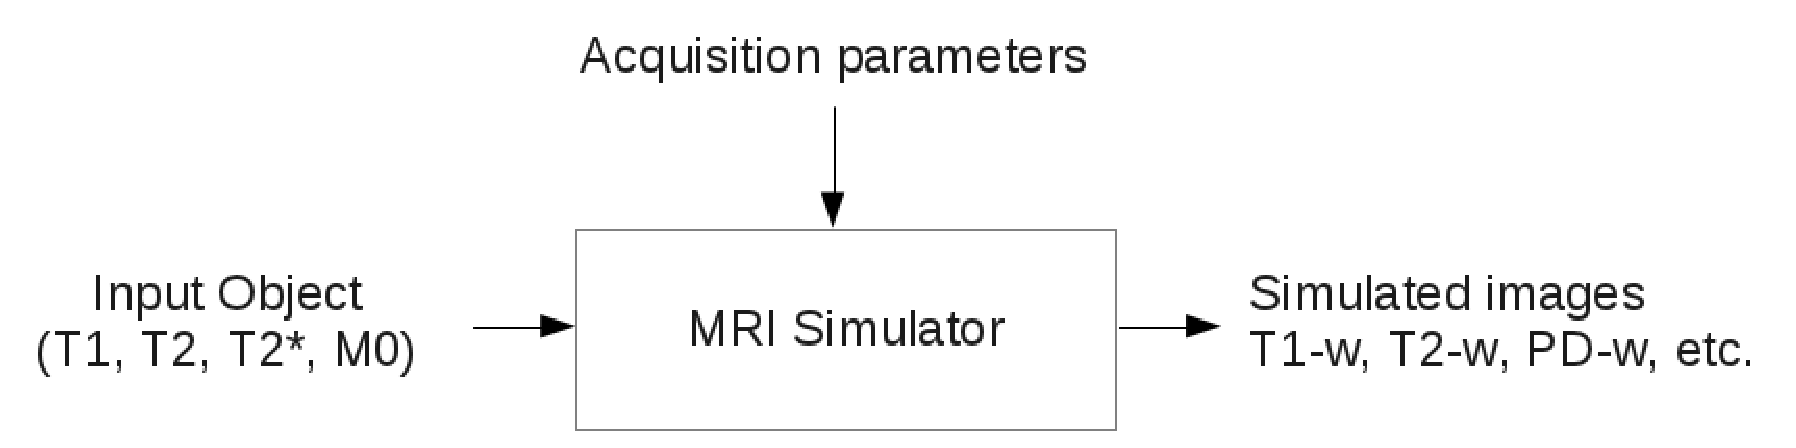
\epsfig{file = simuBloch.eps, width =12cm} 
 \caption[\textit{SimuBloch}]{Simulation workflow for \textit{SimuBloch}. The input object is composed by image volumes of $T1$, $T2$, $T2*$ and $M0$. Depending on the 
			       acquisition parameters, different outputs can be generated.}
 \label{fig:simuBloch}  
\end{figure}

\textit{SimuBloch} is an MRI simulator developed by \cite{caom3}. 
The purpose of \textit{SimuBloch} is to validate 
MRIs of molecular neuro-inflammation within Multiple Sclerosis lesions.

An MR relaxometry technique is used 
to acquire the values of the four physical parameters needed to produce simulated images. 
The parameters are as follows: 

\begin{itemize}
 \item $T1$ or the relaxation constant measuring how fast the spinning nuclei will emit their absorbed RF into the surrounding tissue.
 \item $T2$ or the relaxation constant measuring the time needed for the protons found in water molecules in biological tissue to return to equilibrium.  
 \item $T2*$ or field inhomogeneity. The field inhomogeneity is the principal cause of image distortion and signal loss.
 \item $M0$ or proton density $\rho$, measuring the mobile hydrogen atoms in the tissue. 
\end{itemize}

\textit{SimuBloch} uses the physical parameters of materials to produce simulated images. 
Each of the parameters are provided to \textit{SimuBloch} using 3D images.
Each voxel contains the physical parameter needed to compute the local spin magnetization. % using an improved version of the DESPOT algorithm.

Using the physical parameters, the simulator is able to compute
various types of acquisitions including  
$T1$-weighted, $T2$-weighted, $PD$-weighted, FLAIR, etc. 
similar to the sequences implemented in a real device. 

Figure \ref{fig:simuBloch} explains the workflow of a simulation. 

\textit{SimuBloch} is available to use on the \textit{ VIP}\footnote{\url{http://vip.creatis.insa-lyon.fr/}} platform. 
A test case is available on the \textit{ VIP}. It has three images of physical parameters: $T1$, $T2$, and $M0$. 
Figure \ref{fig:simuBlocPhysical} shows a slice of the image of physical parameters and the result 
of \textit{SimuBloch}. The result image is a $T1$-weighted acquisition with $TR=500$ and $TE=8.4$.

\begin{figure}
 \centering    
 \subfigure[Physical parameters.]{\epsfig{file = SimuBlochPhysicalParameters.eps, width =5cm}}
 \subfigure[Simulated image using \textit{SimuBloch}]{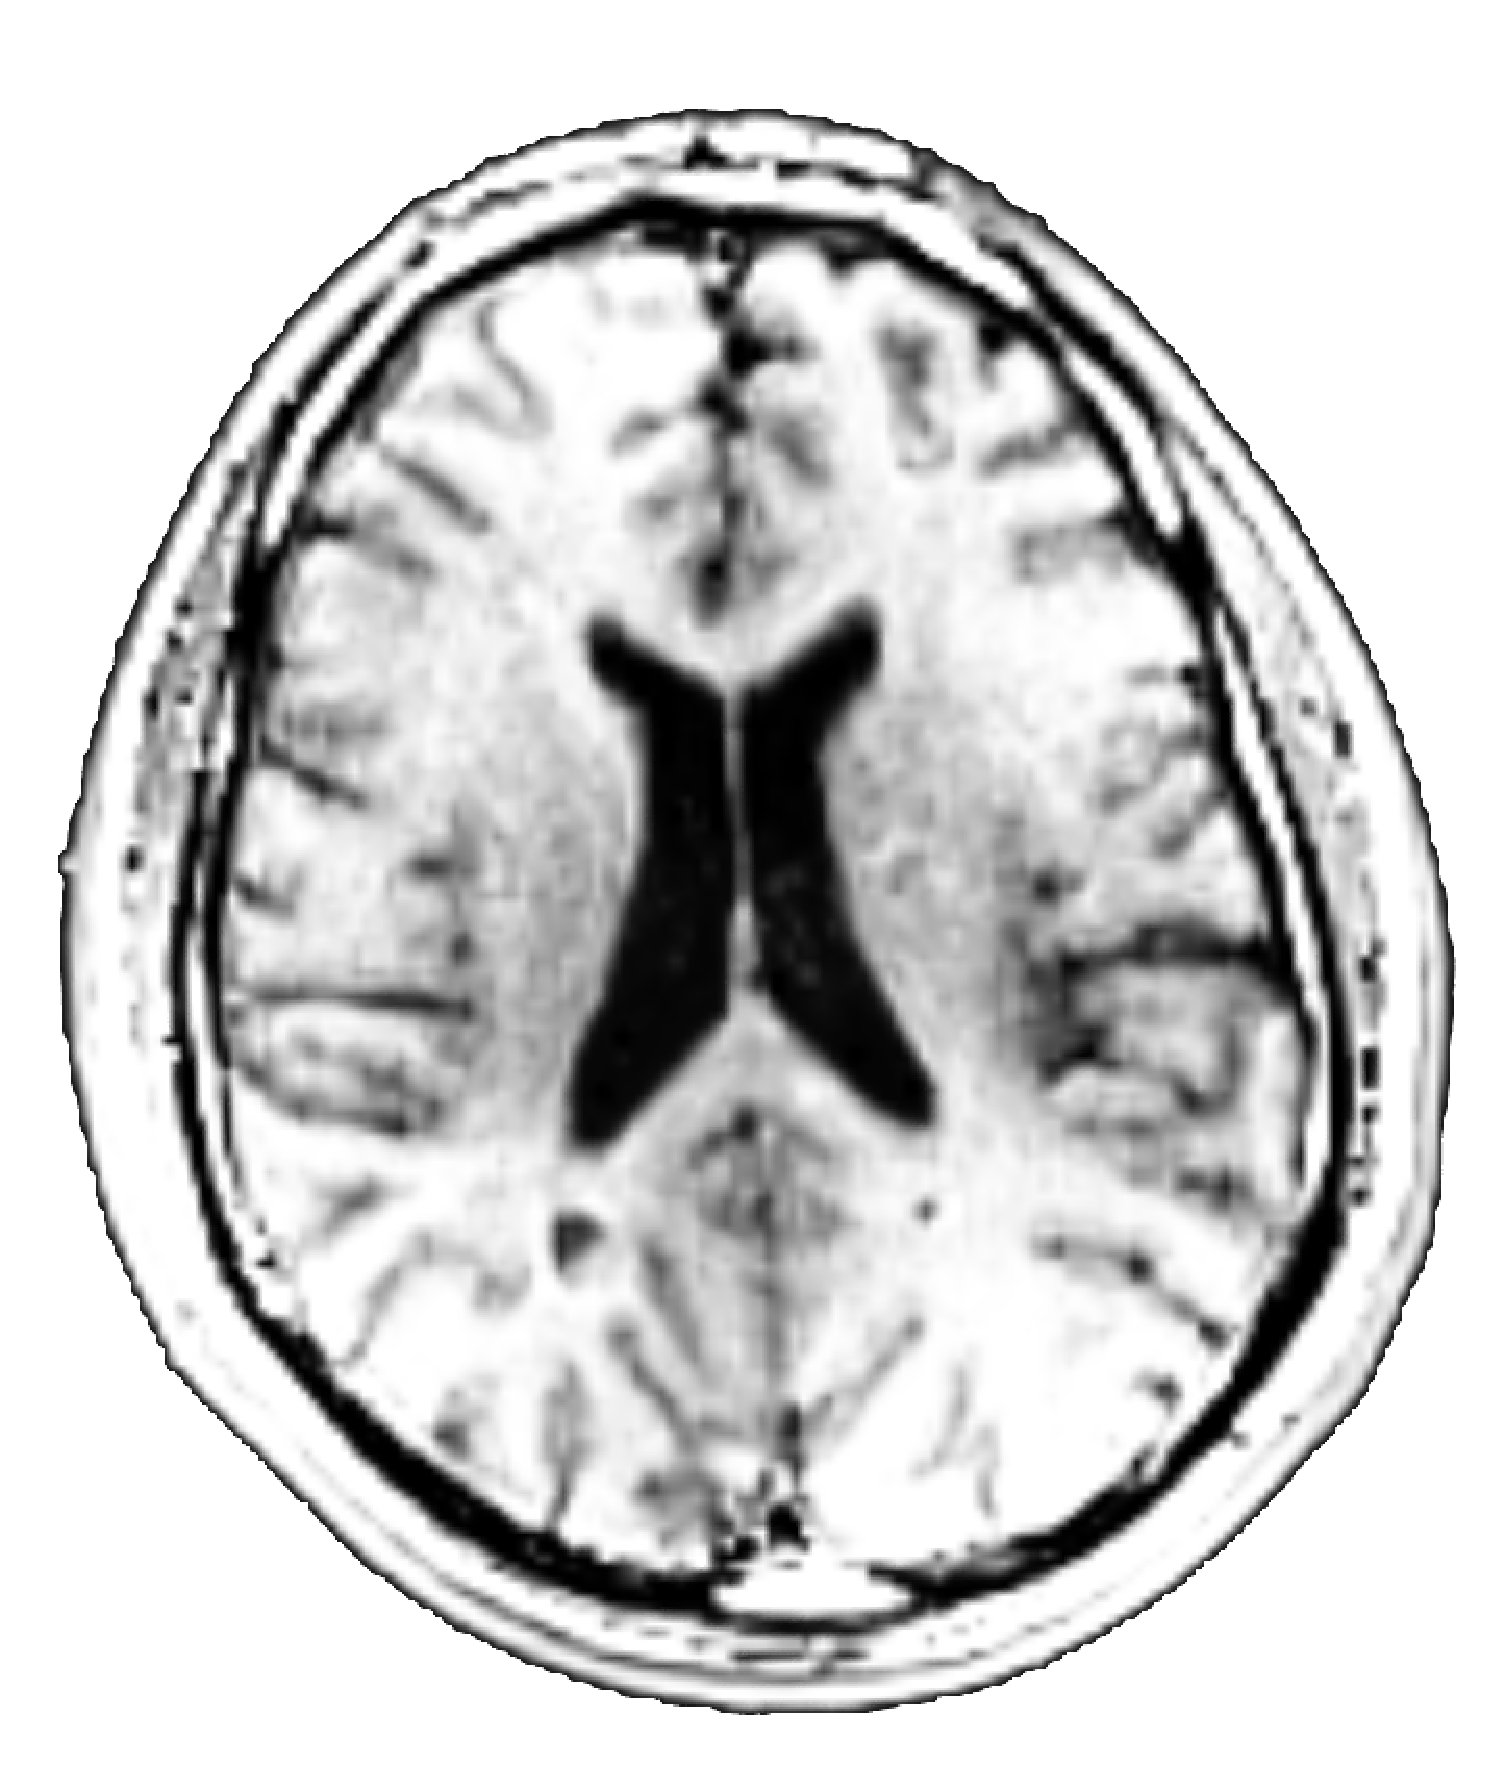
\epsfig{file = SimulatedImageSimuBloch, width =5cm}}
 \caption[\textit{SimuBloch} physical parameters.]{The physical parameters from SimuBloch are composed into a single image. $T1$ is shown in red, $T2$ in green and $M0$ in blue. 
	    All channels are rescaled between $[0-255]$ for visualization purposes.
	    The simulated image is a $T1w$ with acquisition parameters of $TR=500$ $TE=8.4$.
	    }
 \label{fig:simuBlocPhysical}  
\end{figure}


The following section explains how to generate simulated physical parameters images from s-reps 
and solid texture synthesis.


\section{Texturing s-reps}
\label{sec:simulationExperiment}

The texture synthesis algorithm developed in Section \ref{sec:solidTextureImplementation} 
uses 2D textured images to create solid blocks of texture.
The procedure keeps the statistical features of the sample (this was shown in Section \ref{sec:EvaluationTexture})
and some structural features as well.

The solid blocks or cuboids can be warped into an s-rep using an $X2U$ map (see Section \ref{sec:internalCoordinates} for a review on $X2U$ maps and 
the object coordinates $U = [u, v, \tau]$).
The $X2U$ map parameterizes every position inside the s-rep with the $[u, v, \tau]$ coordinate system. 
These coordinates can be modified to map the length, width and height of the cuboid. 
In other words, a function is designed to map every position 
in the s-rep to a position in the cuboid.

The following section explains how the mapping is done.
RGB textures with different patterns are warped 
into s-reps to help understand the procedure.

Section \ref{sec:simulationExperimentPhy} explains how to 
extract 2D samples of physical parameters
that can be used to synthesize solids. 
The resulting solids
are warped to s-rep models in order
to enhance their internal properties
with physical parameters.

The s-rep models are from different subcortical 
structures and the cortex. 
The enhanced representations are used to produce MRI simulated images with \textit{SimuBloch}.

\subsection{Warping RGB textures}
\label{sec:simulationExperimentRGB}

\begin{figure} 
 \centering   
 %\subfigure[Image samples]{\epsfig{file = hippocampusZebraTexture.eps, width =2cm}}
 \subfigure[Mapping the solid texture to the s-rep with the $X2U$ map. 
	    The values of $v$ and $\tau$ are modified to enforce the continuity of the solid inside the object.]{\epsfig{file = explainX2U-b.eps, width=8cm}}
 \subfigure[Volume rendering of an $X2U$ map of the s-rep. The map is sliced to reveal the internal color gradient where 
            the $u$, $v$ and $\tau$ are colored with red, green and blue.]{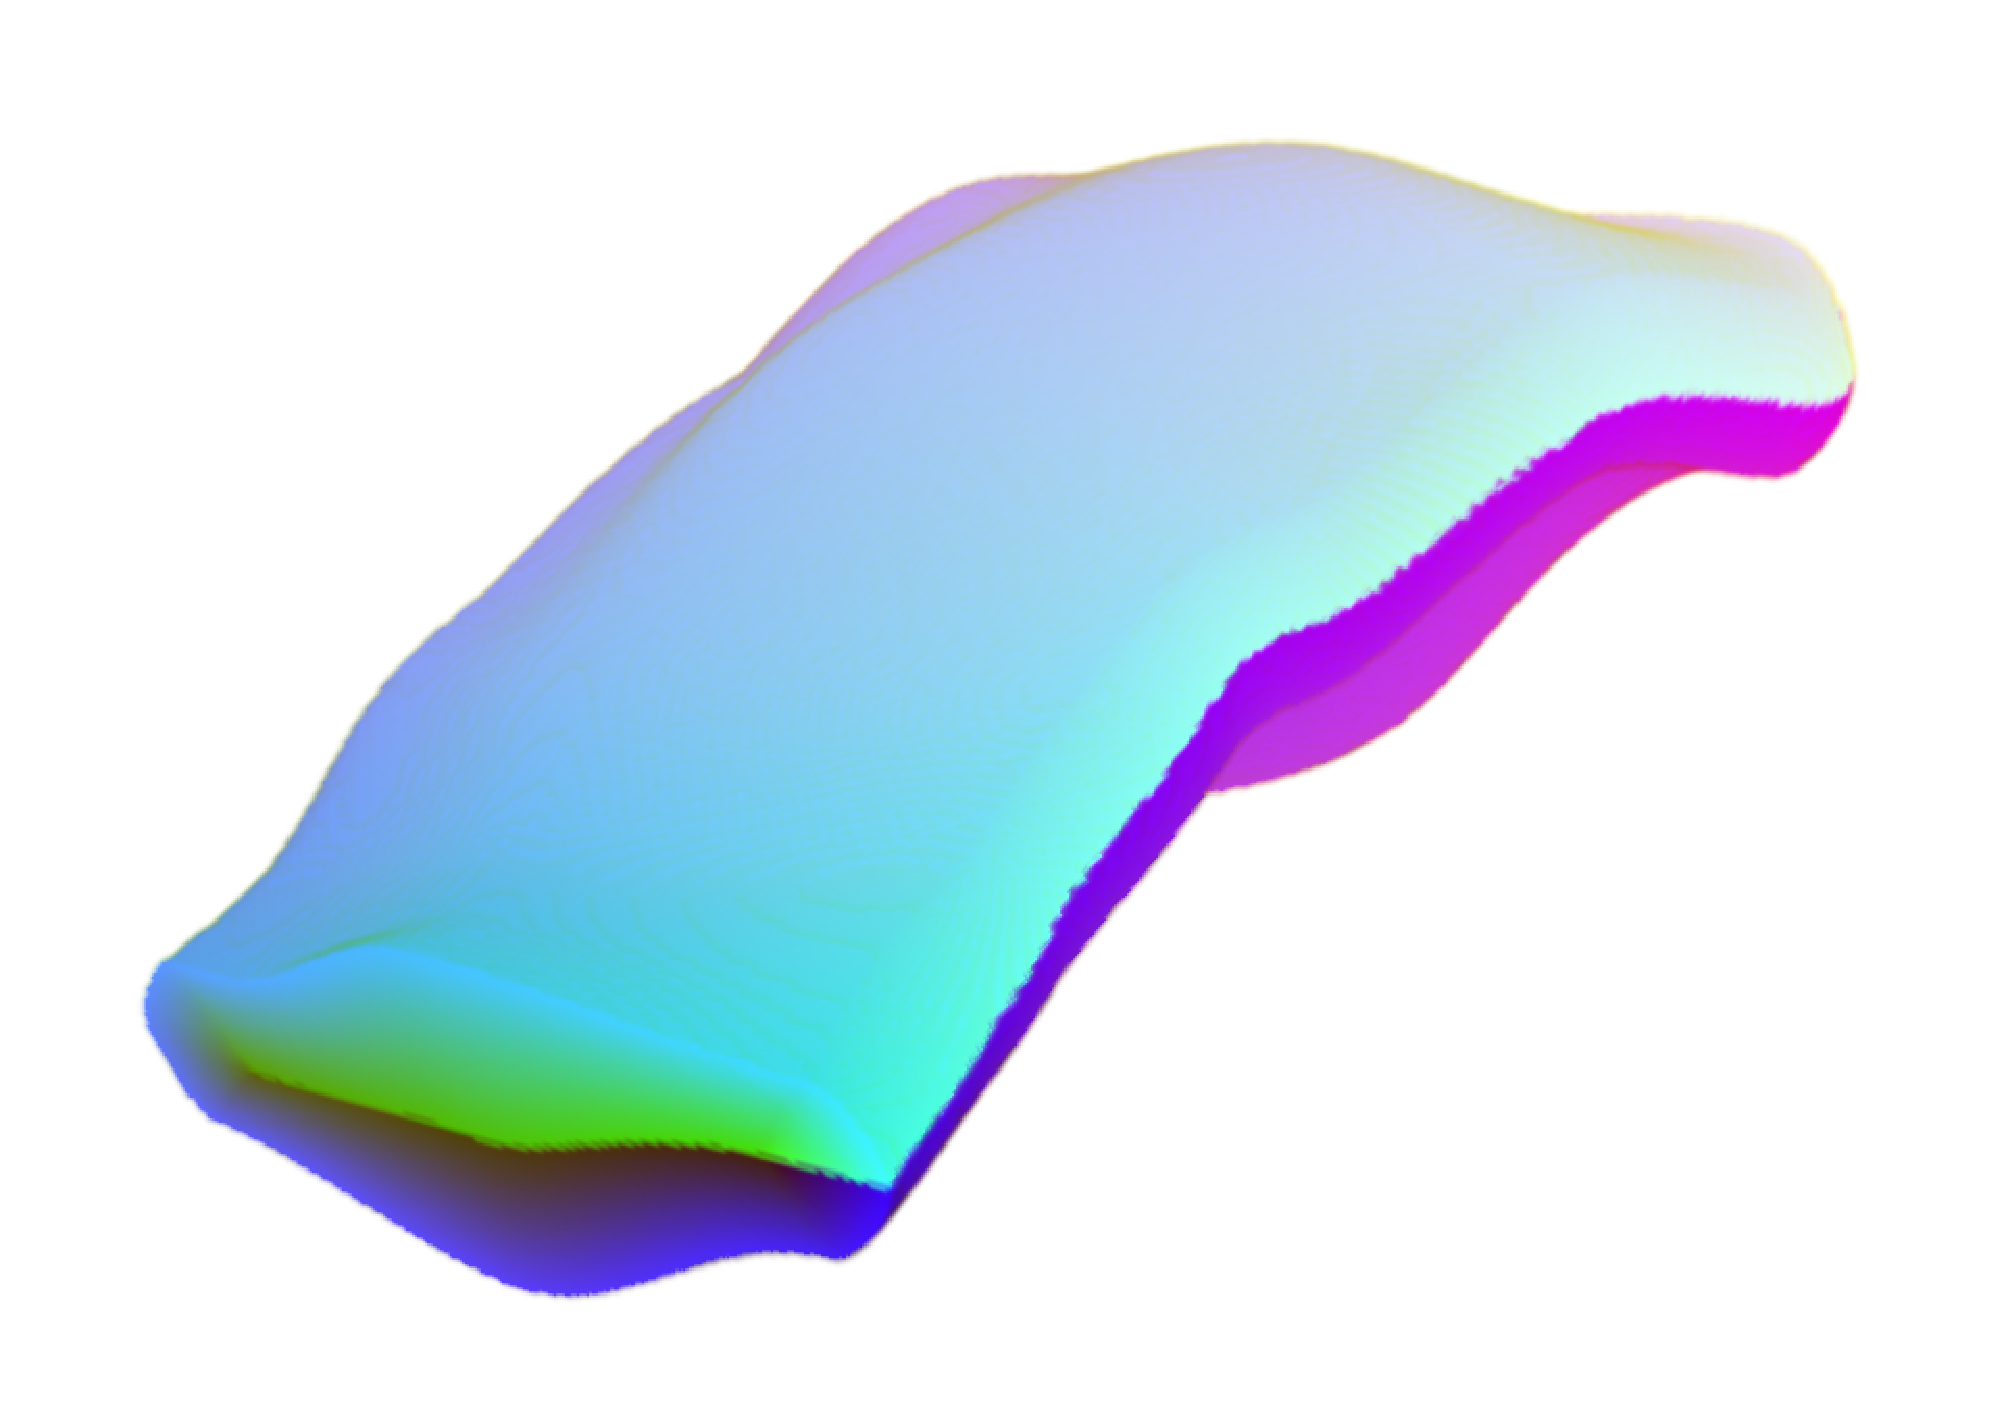
\epsfig{file = explainX2U-c.eps, width=6cm}}
 \caption[Warping a solid texture to an s-rep.]{The $X2U$ map is used to warp the solid texture inside the object. 
                                                The $[u, v, \tau]$ coordinates are transformed into $[u, \hat v, \hat \tau]$ mapping 
						 the length, width and height of the cuboid.}
 \label{fig:texturingS-reps}  
\end{figure}

To warp a solid texture, every position inside the s-rep with coordinates $[u, v, \tau]$ is assigned a corresponding position in a solid block of texture.
Since the synthesis procedure is done inside a cuboid of arbitrary size $(Size_x, Size_y, Size_z)$,
the objective is to design a function $U2C$ such that $U2C(u, v, \tau) = \{ [s_x, s_y, s_z] : s_{x, y, z} \in [0, Size_{x, y, z}] \}$.
In other words, each internal coordinate of the s-rep has a corresponding position in the cuboid.

As explained in Section \ref{sec:internalCoordinates}, there are two functions that allows going 
from world coordinates to object coordinates and vice versa, namely $X2U(x, y, z) = [u, v, \tau]$ and $U2X(u, v, \tau) = [x, y, z]$.
An $X2U$ map stores the coordinates $[u, v, \tau] \in [0, N], N = 1$  of an s-rep at every world coordinate $[x, y, z]$.
%The map provides access from world coordinates to object coordinates in $O(1)$.
Recall that in object coordinates, $v$ wraps around the object ($v \in [0, 0.5]$ for the top side of the s-rep and 
$v \in [0.5, 1]$ for the bottom side of the s-rep) 
and $\tau$ maps from $\tau = 0$ at the SS (skeletal sheet) to the object's boundary at $\tau = 1$.

The function $U2C$ uses a modified version of the $v$ and $\tau$ coordinates
in order to provide continuity of the solid texture inside the s-rep. 
$v$ is modified to map the top and bottom sides of the object to the width of the solid,
and $\tau$ is modified to start at half the height of the cuboid.
The top side of the s-rep will map to the upper part of the cuboid
while the bottom side of the s-rep will map to the lower part of the cuboid. 
This is done in two steps: mapping $v$ and $\tau$ to the variables $\hat v$ and $\hat \tau$ 
and then mapping $[u, \hat v, \hat \tau]$ to $[s_x, s_y, s_z]$.

$\hat v$ and $\hat t$
map to the width and height of the cuboid 
as shown in Equations \ref{equ:modX2Uv} and \ref{equ:modX2Uv} respectively. 
Both transformations depend on the side of the skeletal sheet parameterized by $v < 0.5$ for the top 
and $v > 0.5$ for the bottom.
The $u$ coordinate is not modified and maps the length of the cuboid.

Figure \ref{fig:texturingS-reps}-a shows 
how to modify the $[u, v, \tau]$ coordinates. Figure \ref{fig:texturingS-reps}-b
shows the volume rendering of the $X2U$ map where
the coordinates $[u, v, \tau]$ are colored with red, green and blue respectively (the $X2U$ map is sliced to reveal the internal gradient). 

The size $(Size_x, Size_y, Size_z)$ of the cuboid should be chosen according to the s-rep physical dimensions. 
This is done to preserve the structural information of the texture as it 
might be distorted during the texture warp. This issue arises when the cuboid and the s-rep differ in physical size.
Equation \ref{equ:modX2UWarp} 
shows how to modify the coordinates according to the solid's size.


\begin{equation}
 \hat{v} = \left \{ \begin{array}{ll} 
                     2v,  & v < 0.5 \\
                     2(1 - v), & otherwise
                    \end{array} \right .
  \label{equ:modX2Uv}
\end{equation}
\begin{equation}
 \hat{\tau} = \left \{ \begin{array}{ll} 
                     0.5 + \tau/2, & v < 0.5 \\
                     0.5 - \tau/2, & otherwise
                    \end{array} \right .
  \label{equ:modX2Ut}
\end{equation}
\begin{equation}
  U2C(u, v, \tau) = (u, \hat{v}, \hat{\tau}) \left [ \begin{matrix}
							  Size_x & 0 & 0 \\
							  0 & Size_y & 0 \\
							  0 & 0 & Size_z
							\end{matrix} \right ] = [s_x, s_y, s_z]. 
  \label{equ:modX2UWarp}
\end{equation}

The complete set of functions enables going from world coordinates $[x, y, z] {}_{\overrightarrow{{}_{X2U}}} [u, v, \tau]$
to s-rep coordinates
and from s-rep coordinates $[u, v, \tau] {}_{\overrightarrow{{}_{U2C}}} [s_x, s_y, s_z]$
to the cuboid. Therefore, every s-rep internal position has a corresponding position in the solid.
By querying world coordinates, the information in the solid texture can be retrieved
allowing the texture warp.

A solid texture of size $(256, 128, 64)$ was synthesized
and warped to an s-rep.
The structural features are preserved
as shown in Figure \ref{fig:volumeRenderingS-repsText}
with the volume rendering representation. 

Figure \ref{fig:volumeRenderingCortex} shows a volume rendering representation of the cortex using a zebra and a dot texture. 
The size of the solid texture is $[4096, 4096, 32]$. The tubular structure mimics the cortical columns running perpendicular 
to the cortical surface (see Chapter \ref{chapter:cortexModeling} for a review of cortical columns). 

\begin{figure} 
 \centering   
 \subfigure[Sample and volume.]{
\epsfig{file = spheres.eps, width =1.5cm} 
                    \epsfig{file = spheresCuboid.eps, width =4cm}}
 \subfigure[Volume rendering]{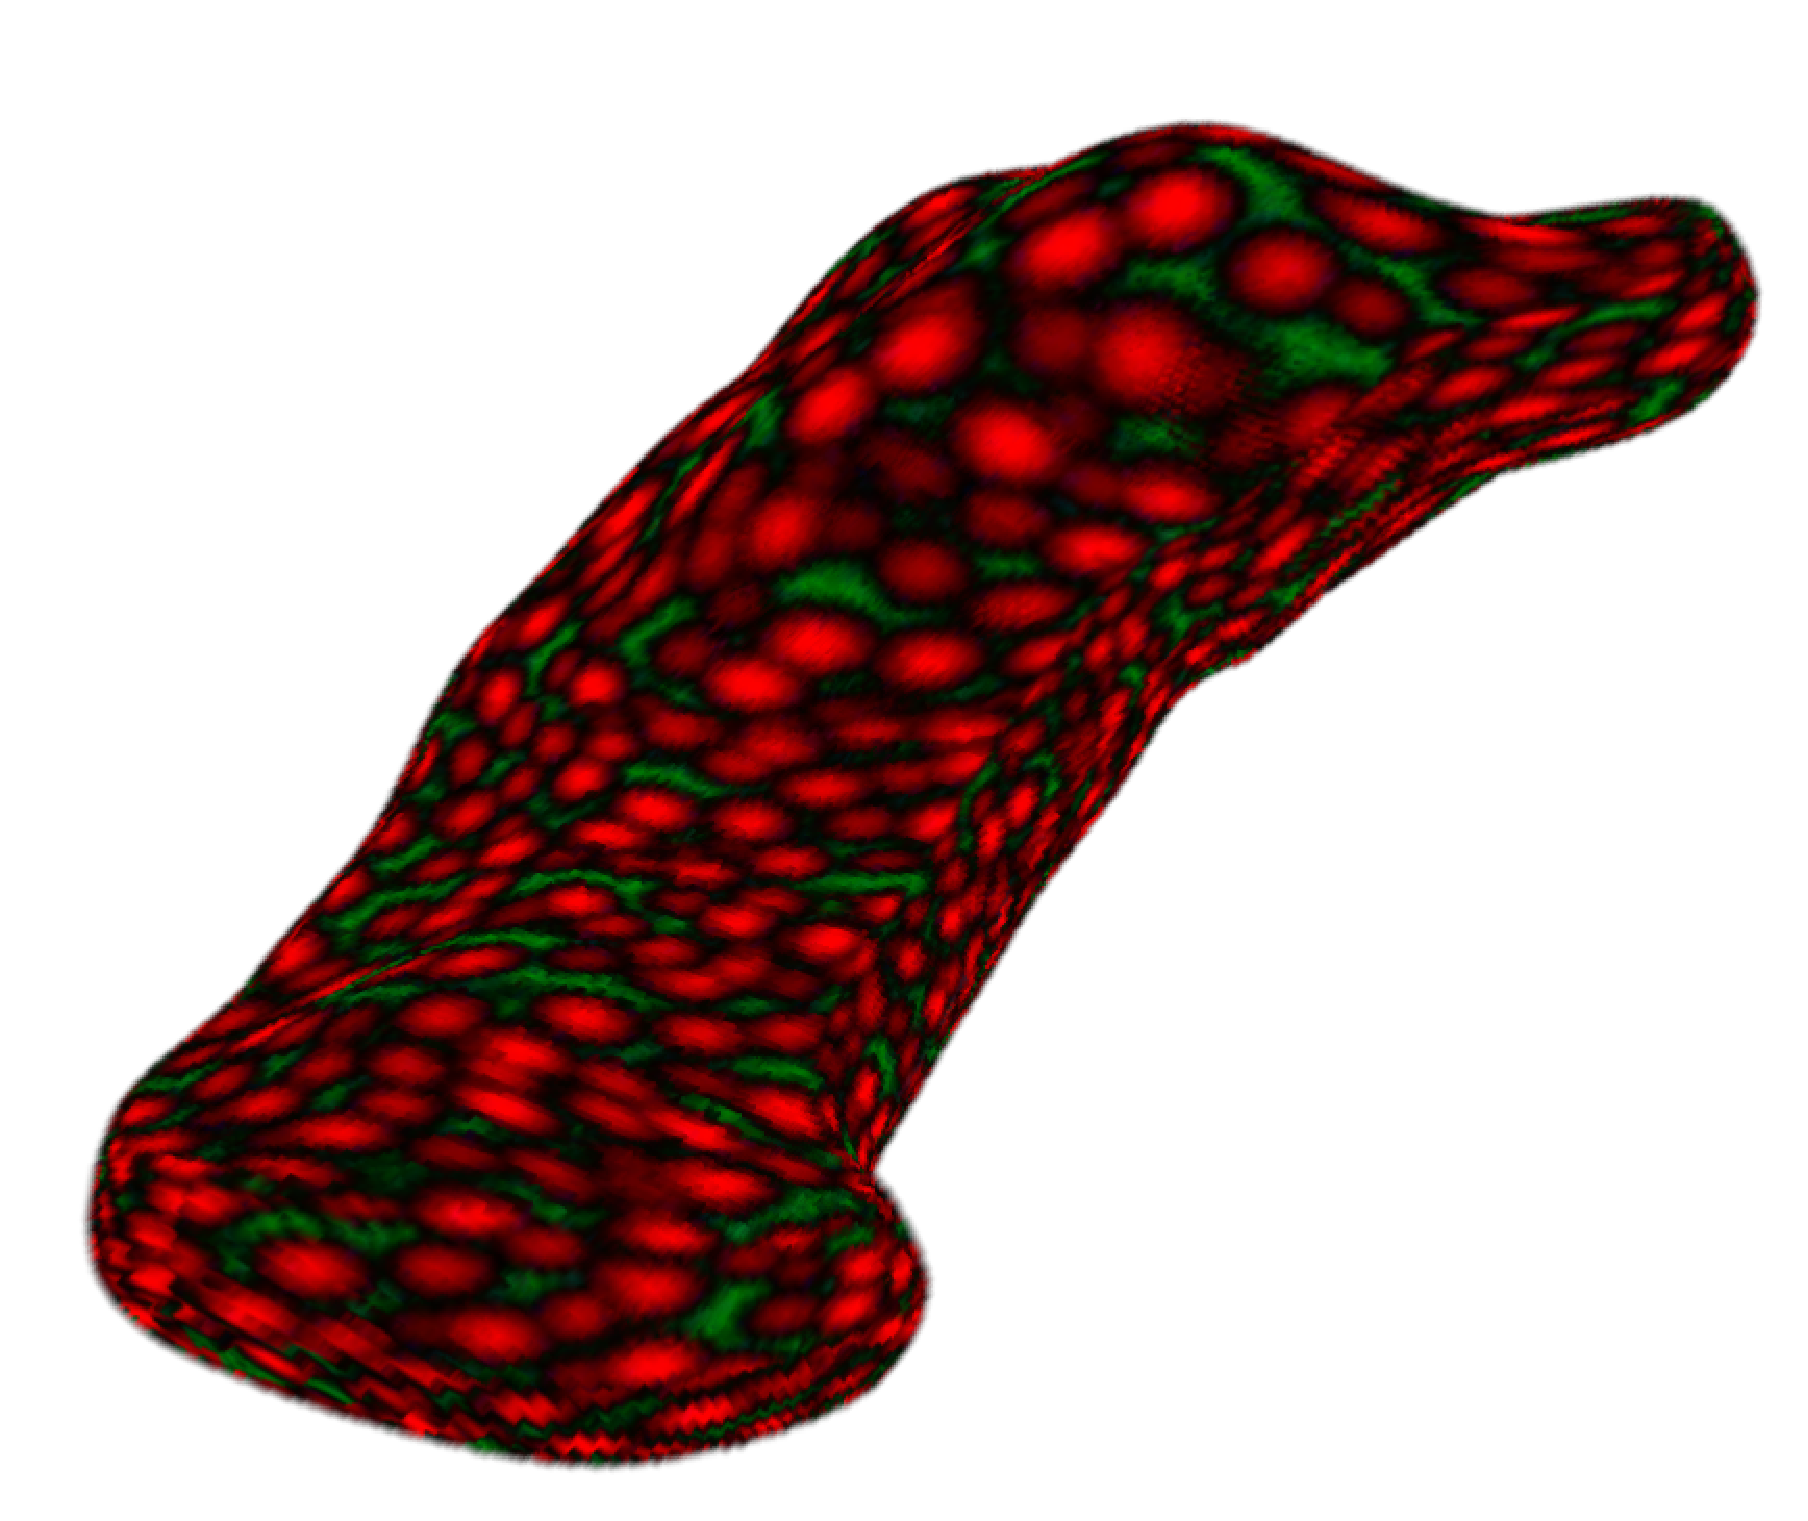
\epsfig{file = spheresVolumeRendering.eps, width =5.5cm}
				           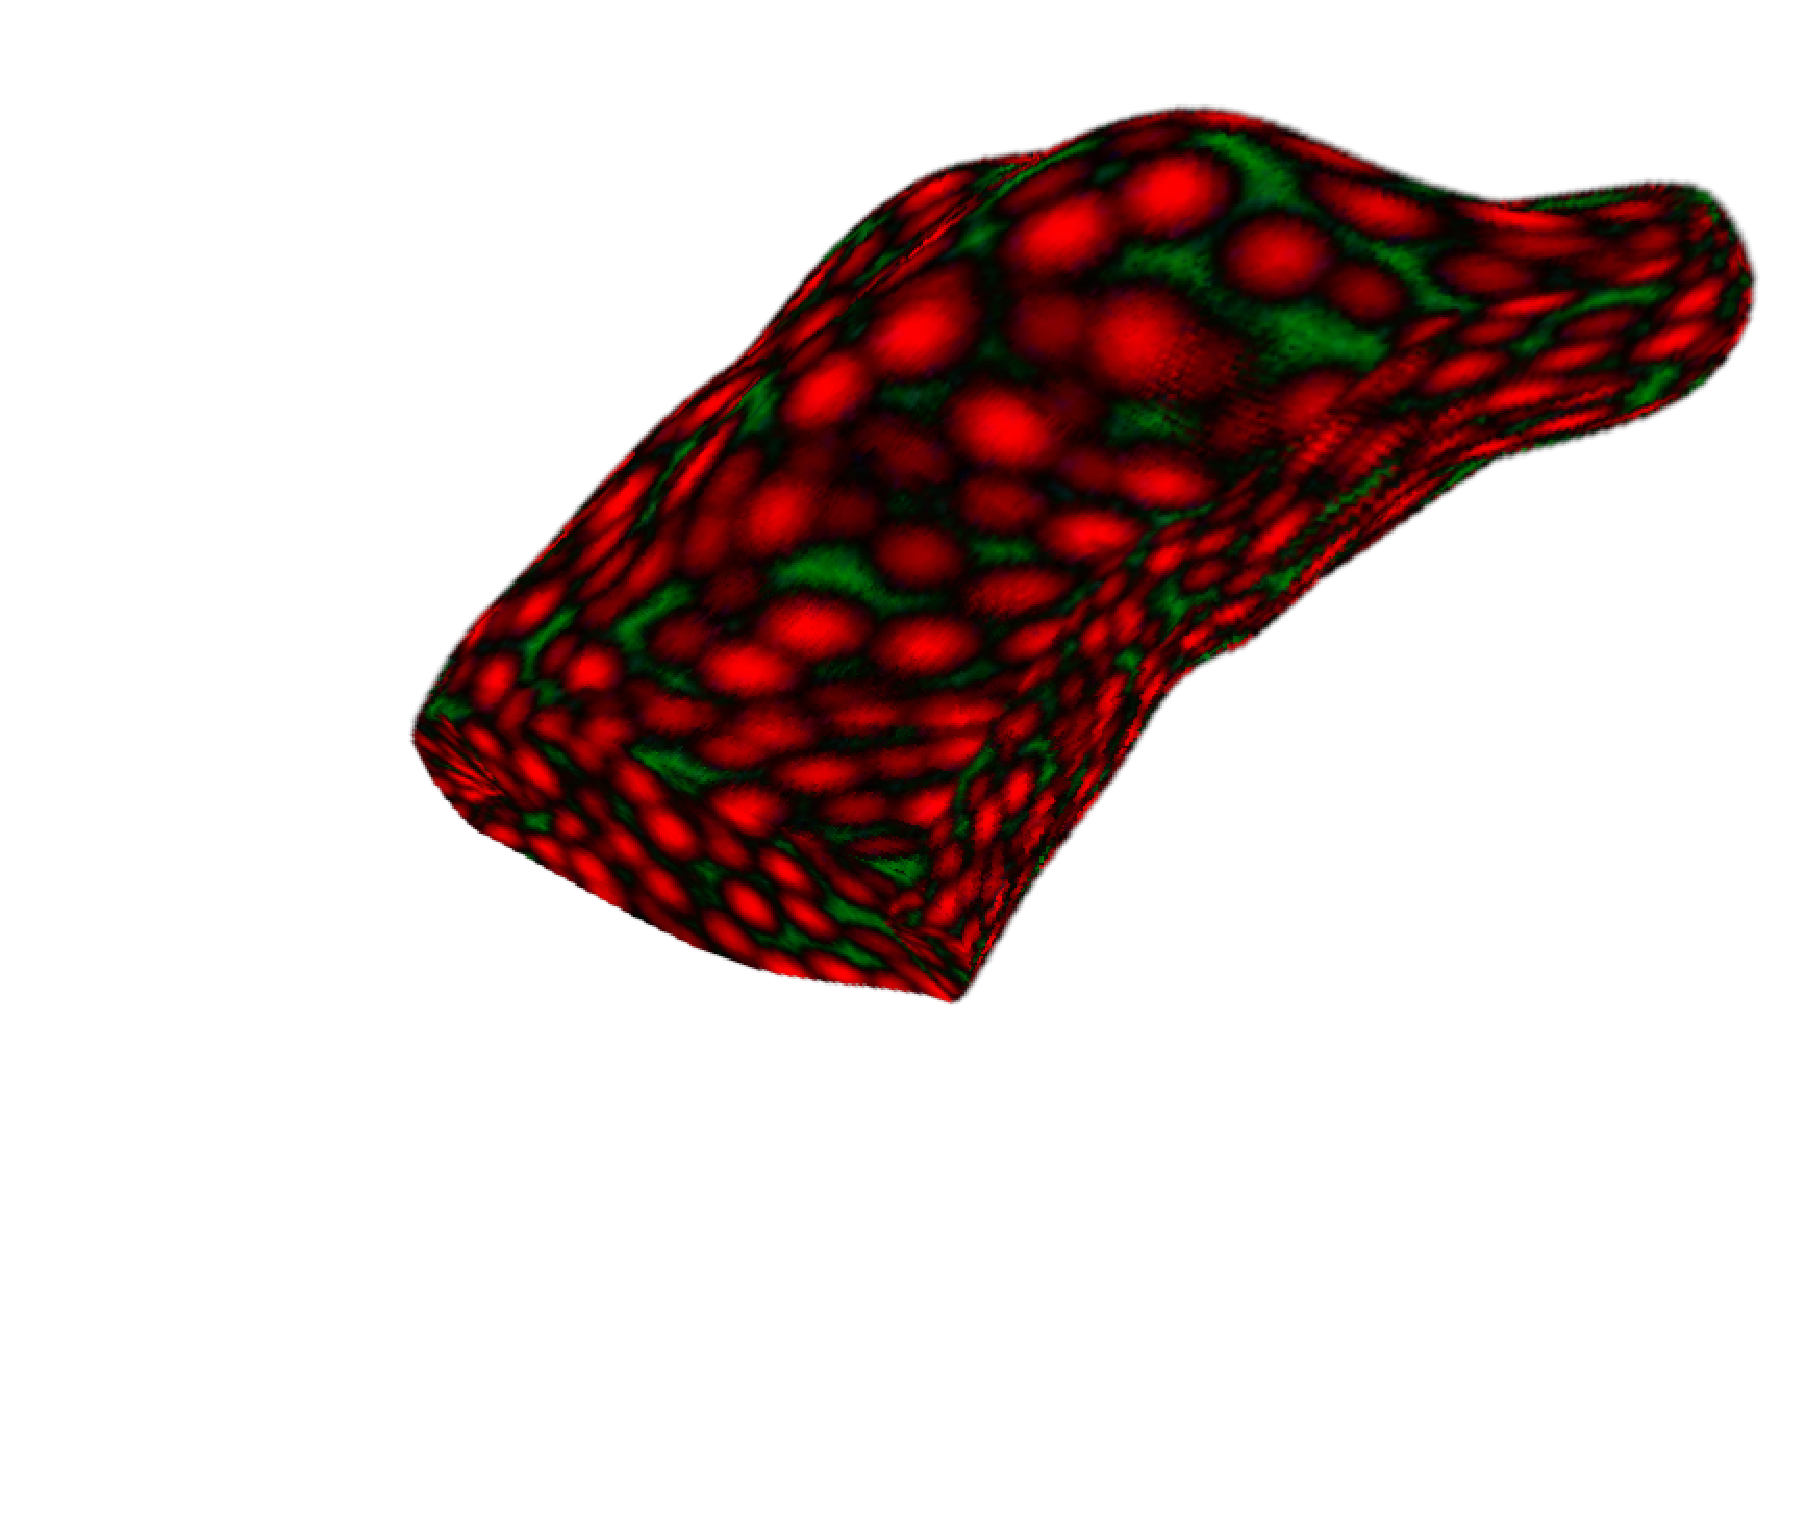
\epsfig{file = spheresVolumeRendering1.eps, width =5.5cm}}   
 \subfigure[Sample and volume.]{
\epsfig{file = striescardiaques.eps, width =1.5cm} 
                    \epsfig{file = striescardiaquesCuboid.eps, width =4cm}}
 \subfigure[Volume rendering]{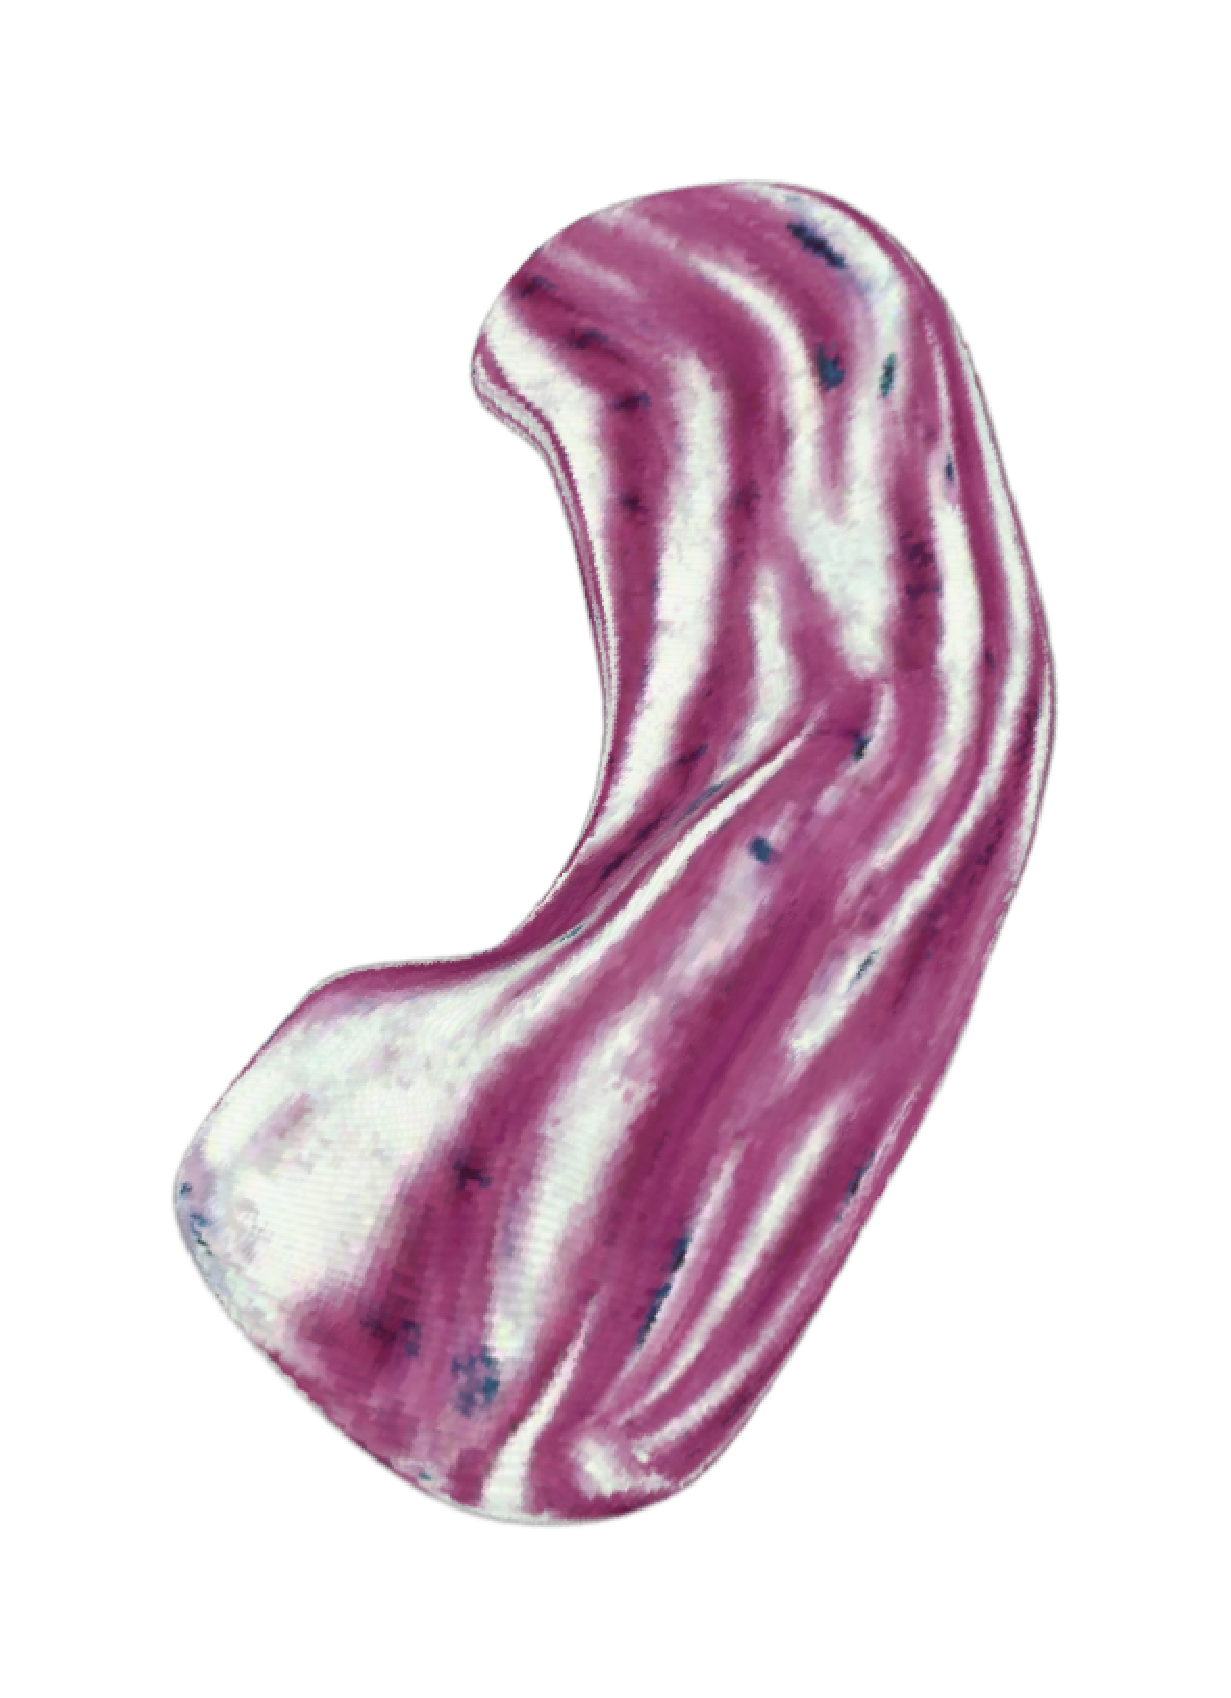
\epsfig{file = stricardiaquesVolumeRendering0.eps, width =5.5cm}
				           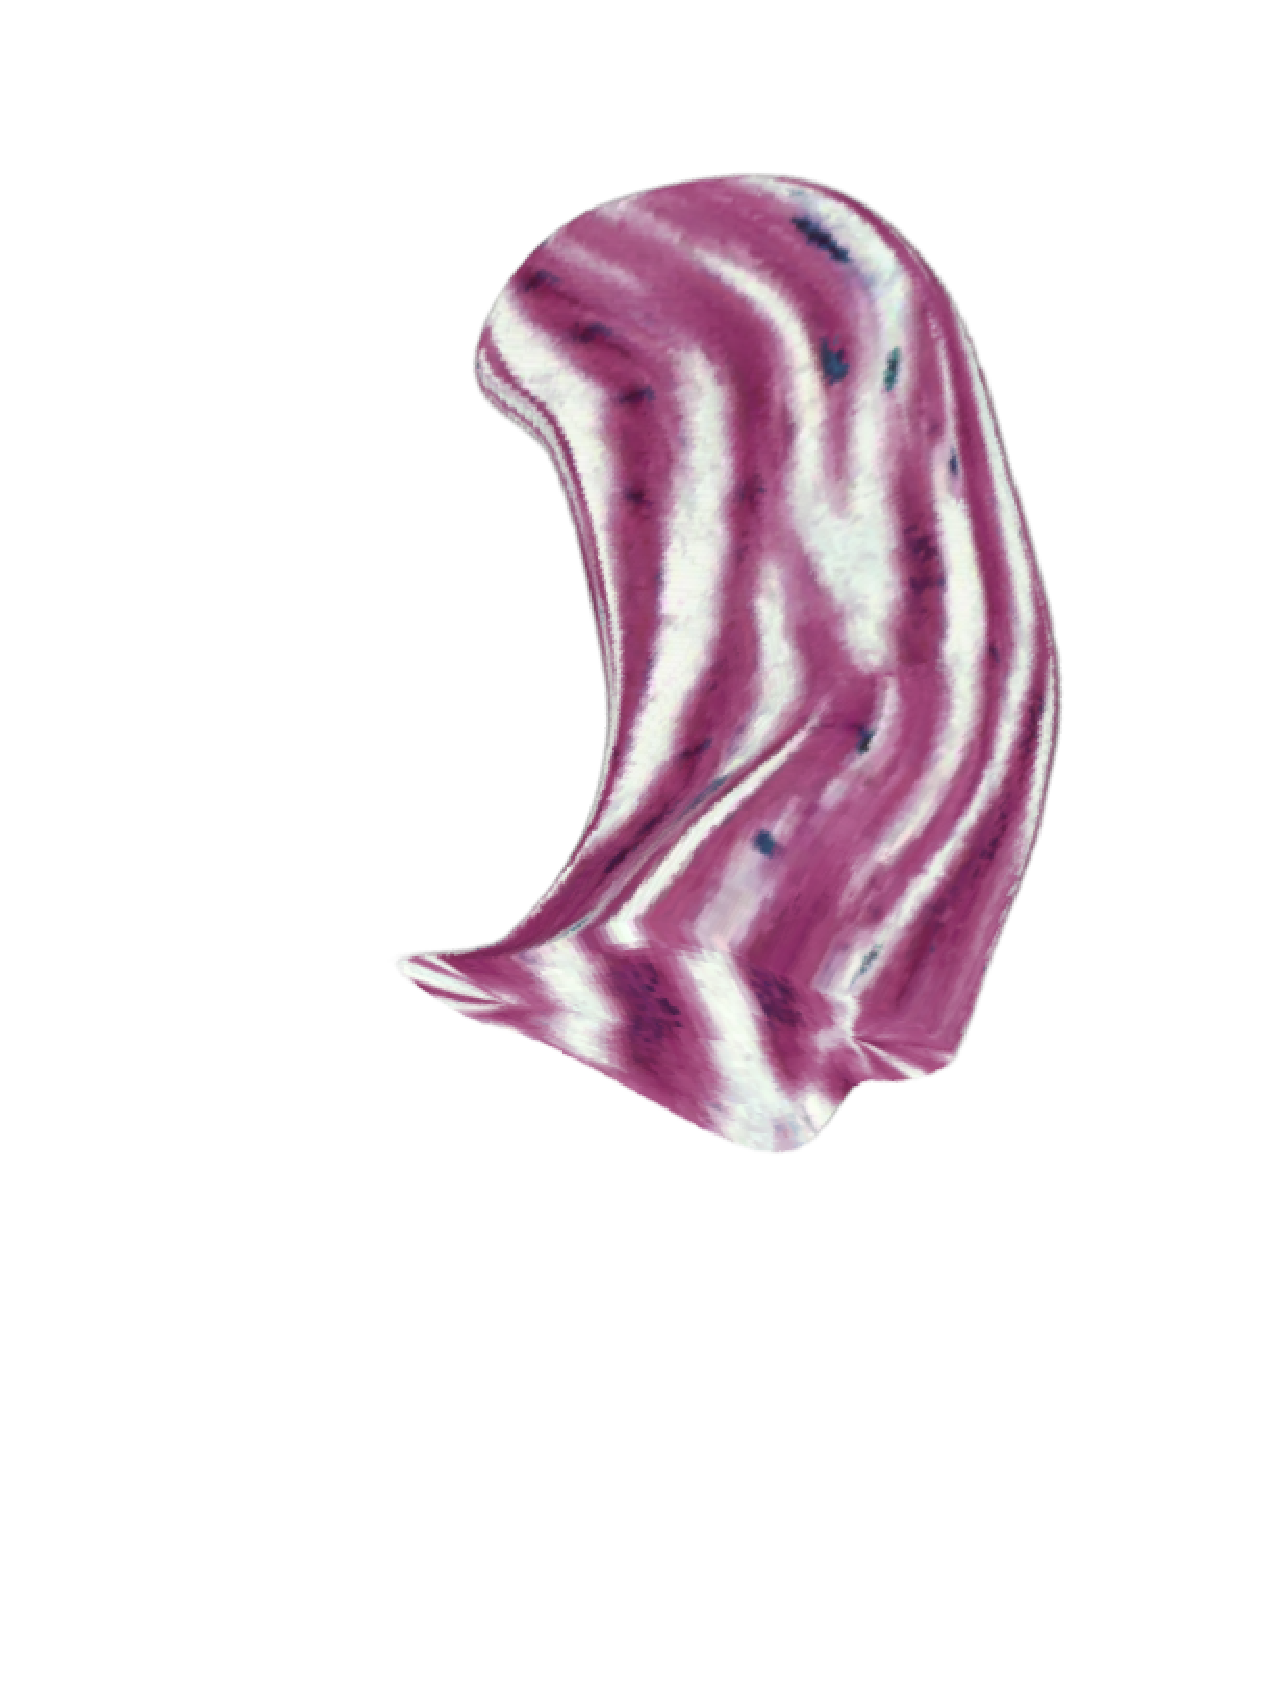
\epsfig{file = stricardiaquesVolumeRendering1.eps, width =5.5cm}} 
 \caption[S-rep textured with spheres and striated cardiac tissue.]{Volume rendering of an textured s-rep. The size of the synthesized texture is $(256, 128, 64)$. 
								     The texture is warped inside the object using the $X2U$ map of the s-rep and 
							             is cut at a random location revealing internal features.}
 \label{fig:volumeRenderingS-repsText}  
\end{figure}

\begin{figure} 
 \centering   
 \subfigure[Samples]{
\epsfig{file = zebra.eps, width =2cm} 
\epsfig{file = zebraAx.eps, width =2cm}}
 \subfigure[Zebra volume]{\epsfig{file = zebraAxVol.eps, width =8cm}} 
 \subfigure[Volume rendering of an s-rep of the cortex using the zebra texture.]{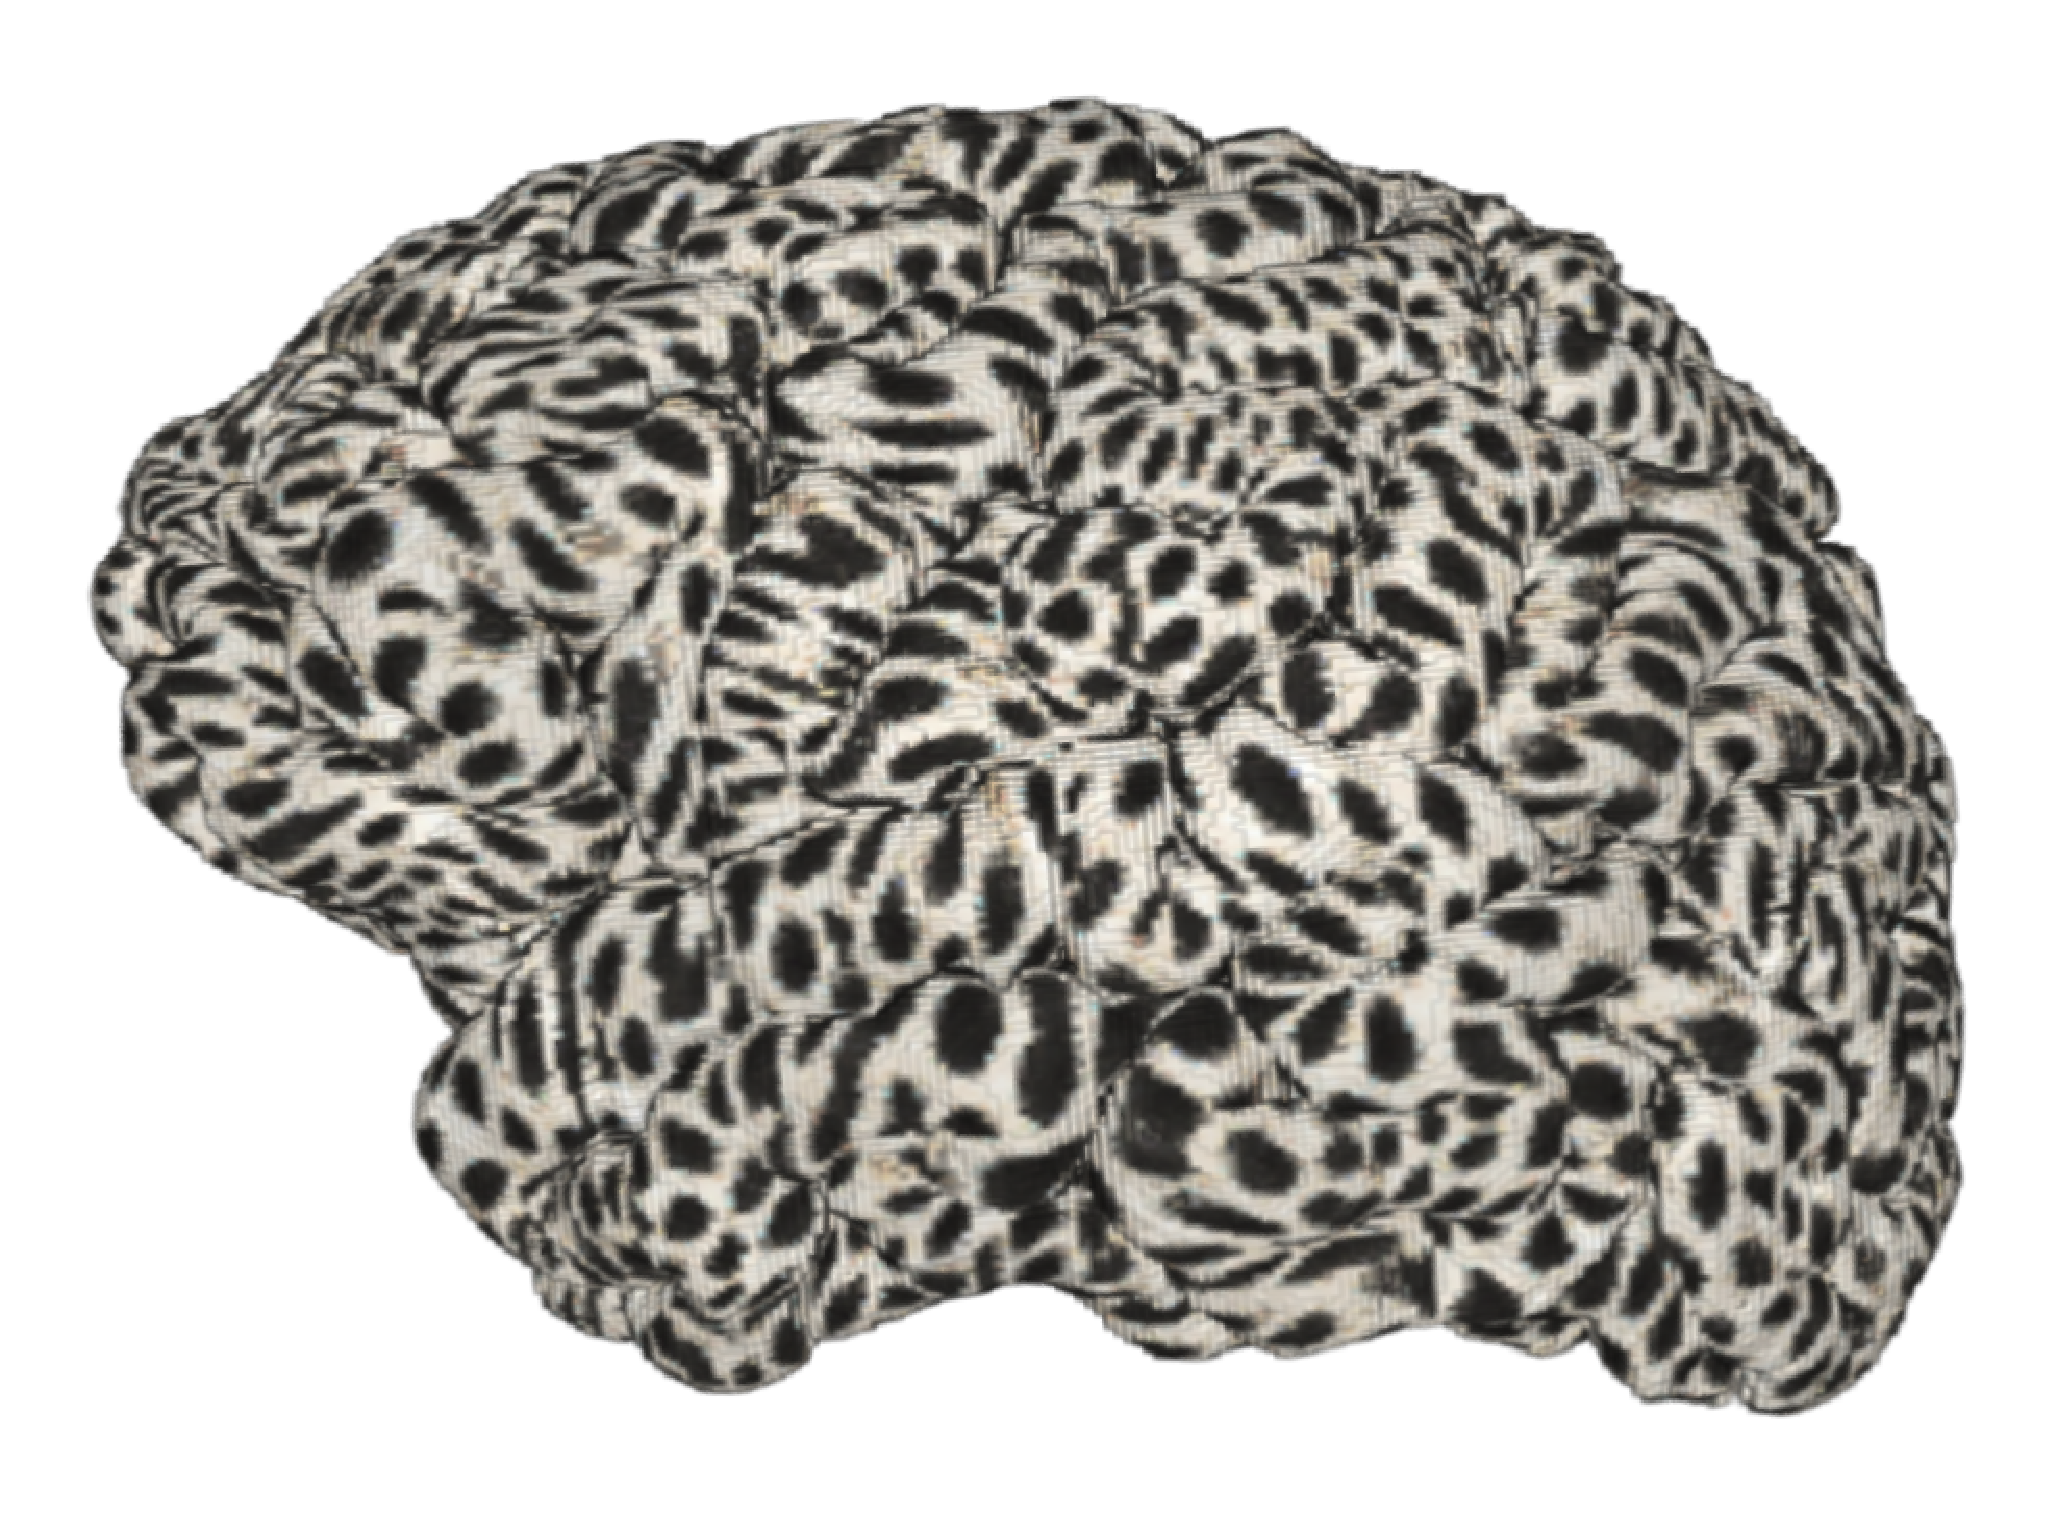
\epsfig{file = zebraAxCortex.eps, width =15cm}} 
 \caption[S-rep of the cortex with zebra texture.]{The size of the synthesized solid is $[4096, 4096, 32]$. The texture is warped inside the object using the $X2U$ map. In this case
						    the cylinders from the texture run perpendicular to the cortical surface. Similar to the cortical columns explained in Chapter \ref{chapter:cortexModeling}.}
 \label{fig:volumeRenderingCortex}  
\end{figure}

The following section explains how to extract 2D samples of physical parameters.
The exemplars are used to generate solid textures that 
can be warped into an s-rep with the procedure just explained.

The s-reps are from the following brain structures:
amygdala, caudate, hippocampus, lateral ventricles, pallidum, putamen and cortex.

Additionally, the s-rep of the cortex is used to locate
the WM (white matter) and cerebral spinal fluid regions in the brain.

Each s-rep and brain region is textured individually,
and then they are merged into a single image. 
The result is a volumetric image with multiple components,
$T1$, $T2$ and $M0$, the parameters
needed to produce a simulated $T1$-weighted image.

\subsection{MRI simulation with textures of physical parameters}
\label{sec:simulationExperimentPhy}

The first step towards MRI simulation is to generate 2D samples of physical parameters.
The exemplars are extracted from a relaxometry image measuring 
the physical properties of brain tissues.
The brain structures considered are the following:
amygdala, caudate, hippocampus, lateral ventricles, pallidum, putamen, cortex, WM and cerebral spinal fluid.
Each of the generated 2D samples 
will be provided to the texture synthesis algorithm in order to create solid textures of physical parameters.

Unfortunately, acquiring accurate exemplars is out of the scope of this dissertation.
For the purpose of demonstrating the capabilities of s-reps and the texture synthesis procedure, 
simple 2D image samples of physical parameters are created from 
a relaxometry acquisition available at \textit{VIP} \cite{caom3}. 

This image of physical parameters shown in Figure \ref{fig:simuBlocPhysical}-a.
Figure \ref{fig:simuBlocPhysical}-b shows the corresponding simulated image with \textit{SimuBloch}.
To locate each brain structure in the image of physical parameters, 
the simulated MRI is segmented with \textit{Freesurfer}. 
The segmentation provides binary masks 
that can be used to locate the subcortical structures, the cortex, the WM and the cerebral spinal fluid.

The 2D samples are created by  
randomly choosing a position inside the brain structure (with help of the binary mask) and
copying neighborhoods of size $3\times3$ to the image sample. 
The procedure continues until the exemplar is covered completely.

Figure \ref{fig:physicalParamsSamples} shows the exemplars of physical parameters, the size of the images is $128^2$ pixels.
\begin{figure} 
 \centering   
 \subfigure[Amygdala]{\epsfig{file = amygdala_Sample.eps, width =2cm}}
 \subfigure[Caudate]{\epsfig{file = caudate_Sample.eps, width =2cm}}
 \subfigure[Cortex]{\epsfig{file = cerebral_Cortex_Sample.eps, width =2cm}}
 \subfigure[Lateral ventricle]{\epsfig{file = lateral_Ventricle_Sample.eps, width =2cm}}
 \subfigure[Pallidum]{\epsfig{file = pallidum_Sample.eps, width =2cm}} 
 \subfigure[Putamen]{\epsfig{file = putamen_Sample.eps, width =2cm}}  
 \caption[Image samples of physical parameters]{Samples of physical parameters for the brain structures. The noise from the samples is reduced with a Gaussian filter ($\sigma = 0.5$).}
 \label{fig:physicalParamsSamples}  
\end{figure}
All the generated exemplars are used to synthesize solid textures.
%The solid textures of physical parameters are applied to s-reps of brain 
%structures in order to enhance their internal properties.
%The following structures are modeled with s-reps: amygdala, caudate, hippocampus, lateral ventricles, pallidum, putamen and cortex.

S-reps of subcortical structures are fitted to three different datasets previously segmented by \textit{Freesurfer}.
The fitting procedure is described in Section \ref{sec:quasiMedial}.
The hemispheres of the cortex are generated with the procedure described in 
Section \ref{sec:s-repFittingCortex}.

As mentioned before, the s-rep of the cortex 
is used to locate the region corresponding to the WM. 
To locate this region, the $X2U$ map of the cortex 
is extended in the $\tau$ direction. In other words, the outside region of the 
cortex is coded with $\tau > 1$. 

Recall that the $v$ coordinate codes the top and bottom regions of the s-rep.
For values of $v < 0.5$ and $\tau > 1$ we can reach the folds produced by the GM surface, 
and for $v > 0.5$ and $\tau > 1$ we can reach the WM region.
Using the extended $X2U$ map, the WM region is located and a binary image that has the shape of the WM
is generated.

The binary mask can be used to ``carve'' WM texture out of the cuboid. 
The cuboid has equal size to the binary image of the WM region
and all non-zero voxels are textured with the information in the cuboid.

The outer region of the implied GM surface is textured with cerebral spinal fluid in a similar manner.

\begin{figure} 
 \centering   
 \subfigure[Colored s-reps of subcortical structures.]{\epsfig{file = multiobject.eps, width =7cm}}
 \subfigure[Textured s-reps of subcortical structures with physical parameters.]{\epsfig{file = multiobjectTexturedPhysical.eps, width =7cm}} 
 \subfigure[Textured right hemisphere.]{\epsfig{file = right_cerebral_Cortex_Texture.eps, width =7cm}} 
 \subfigure[Textured left hemisphere.]{\epsfig{file = left_cerebral_Cortex_Texture.eps, width =7cm}}
 \caption[Multi object subcortical]{Multi-object complex of sub-cortical structures for the left and right hemispheres. 
				    The subcortical structures shown are: amygdala, caudate, hippocampus, 
				    lateral ventricle, putamen and pallidum. 
				    They are shown respectively in Figure (a) in colors: red, blue, yellow, cyan, dark yellow and green. 
				    Figure (b) shows the textured s-reps with physical parameters.
				    Figures (c) and (d) show the right and left hemispheres of the cortex.}
 \label{fig:physicalParamsObjects}  
\end{figure}

All textured objects are merged into a single 3D image in the following order:
WM, cerebral spinal fluid, cortex and subcortical structures.
The resulting volume has three components ($T1, T2$ \textit{and} $M0$) and the geometry of the brain structures.
\textit{SimuBloch} can produce a simulated $T1$-weighted image using the generated volume of physical parameters.

Figure \ref{fig:physicalParamsObjectsImage} shows three cases to test the simulation procedure.
\begin{figure} 
 \centering   
 \subfigure[Subject 1]{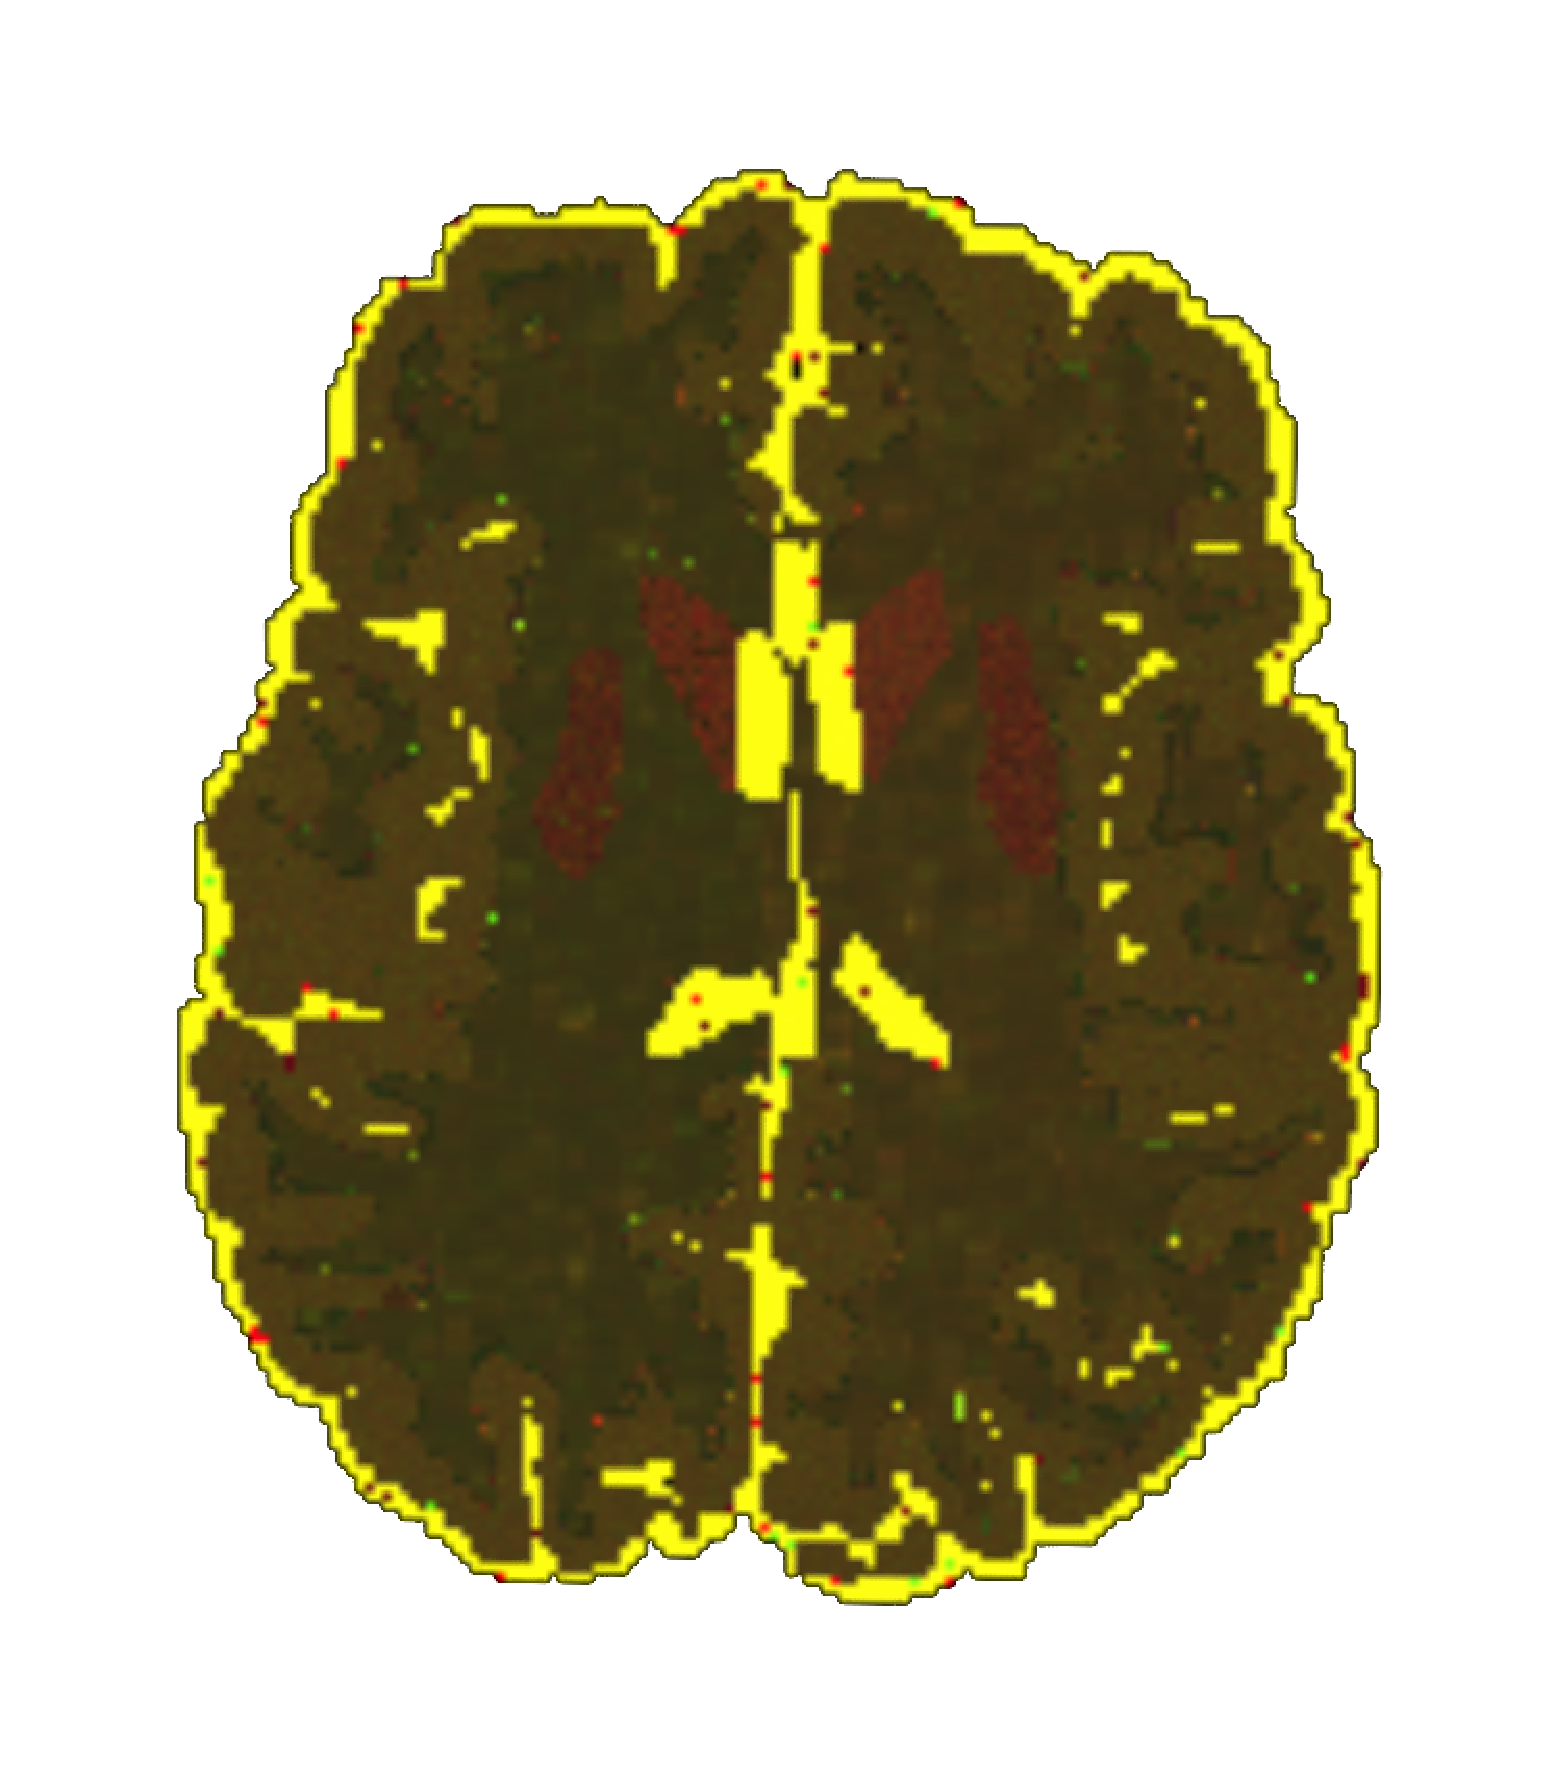
\epsfig{file = SynthPhysicalParameters.eps, width =7cm}}
 \subfigure[Subject 2]{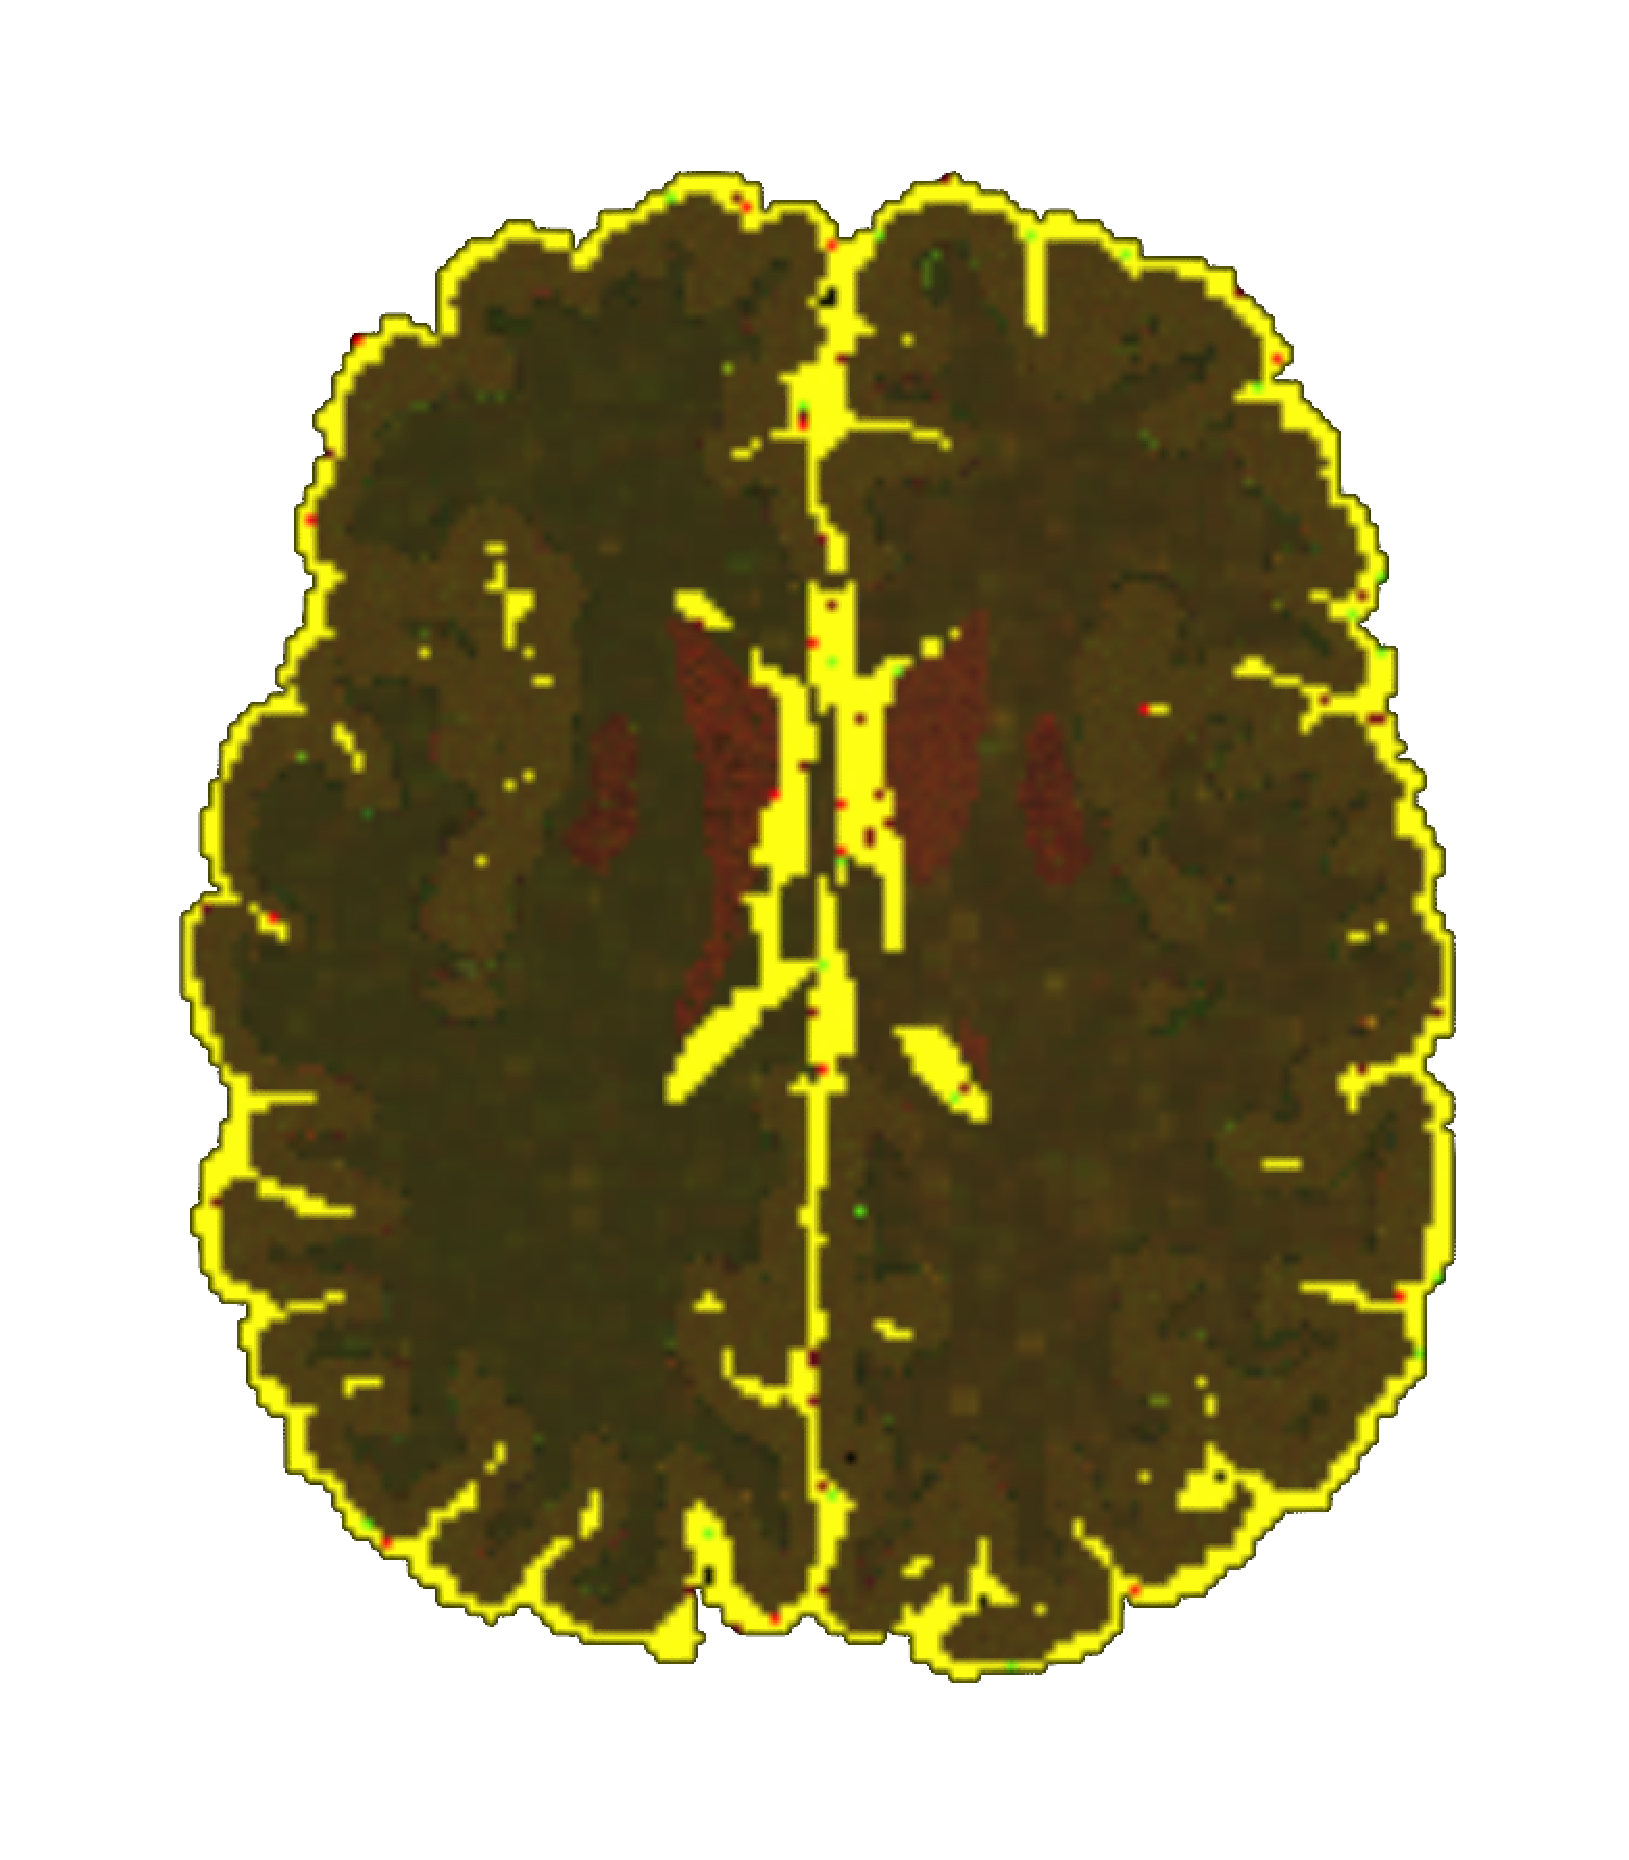
\epsfig{file = SynthPhysicalParameters0.eps, width =7cm}}
 \subfigure[Subject 3]{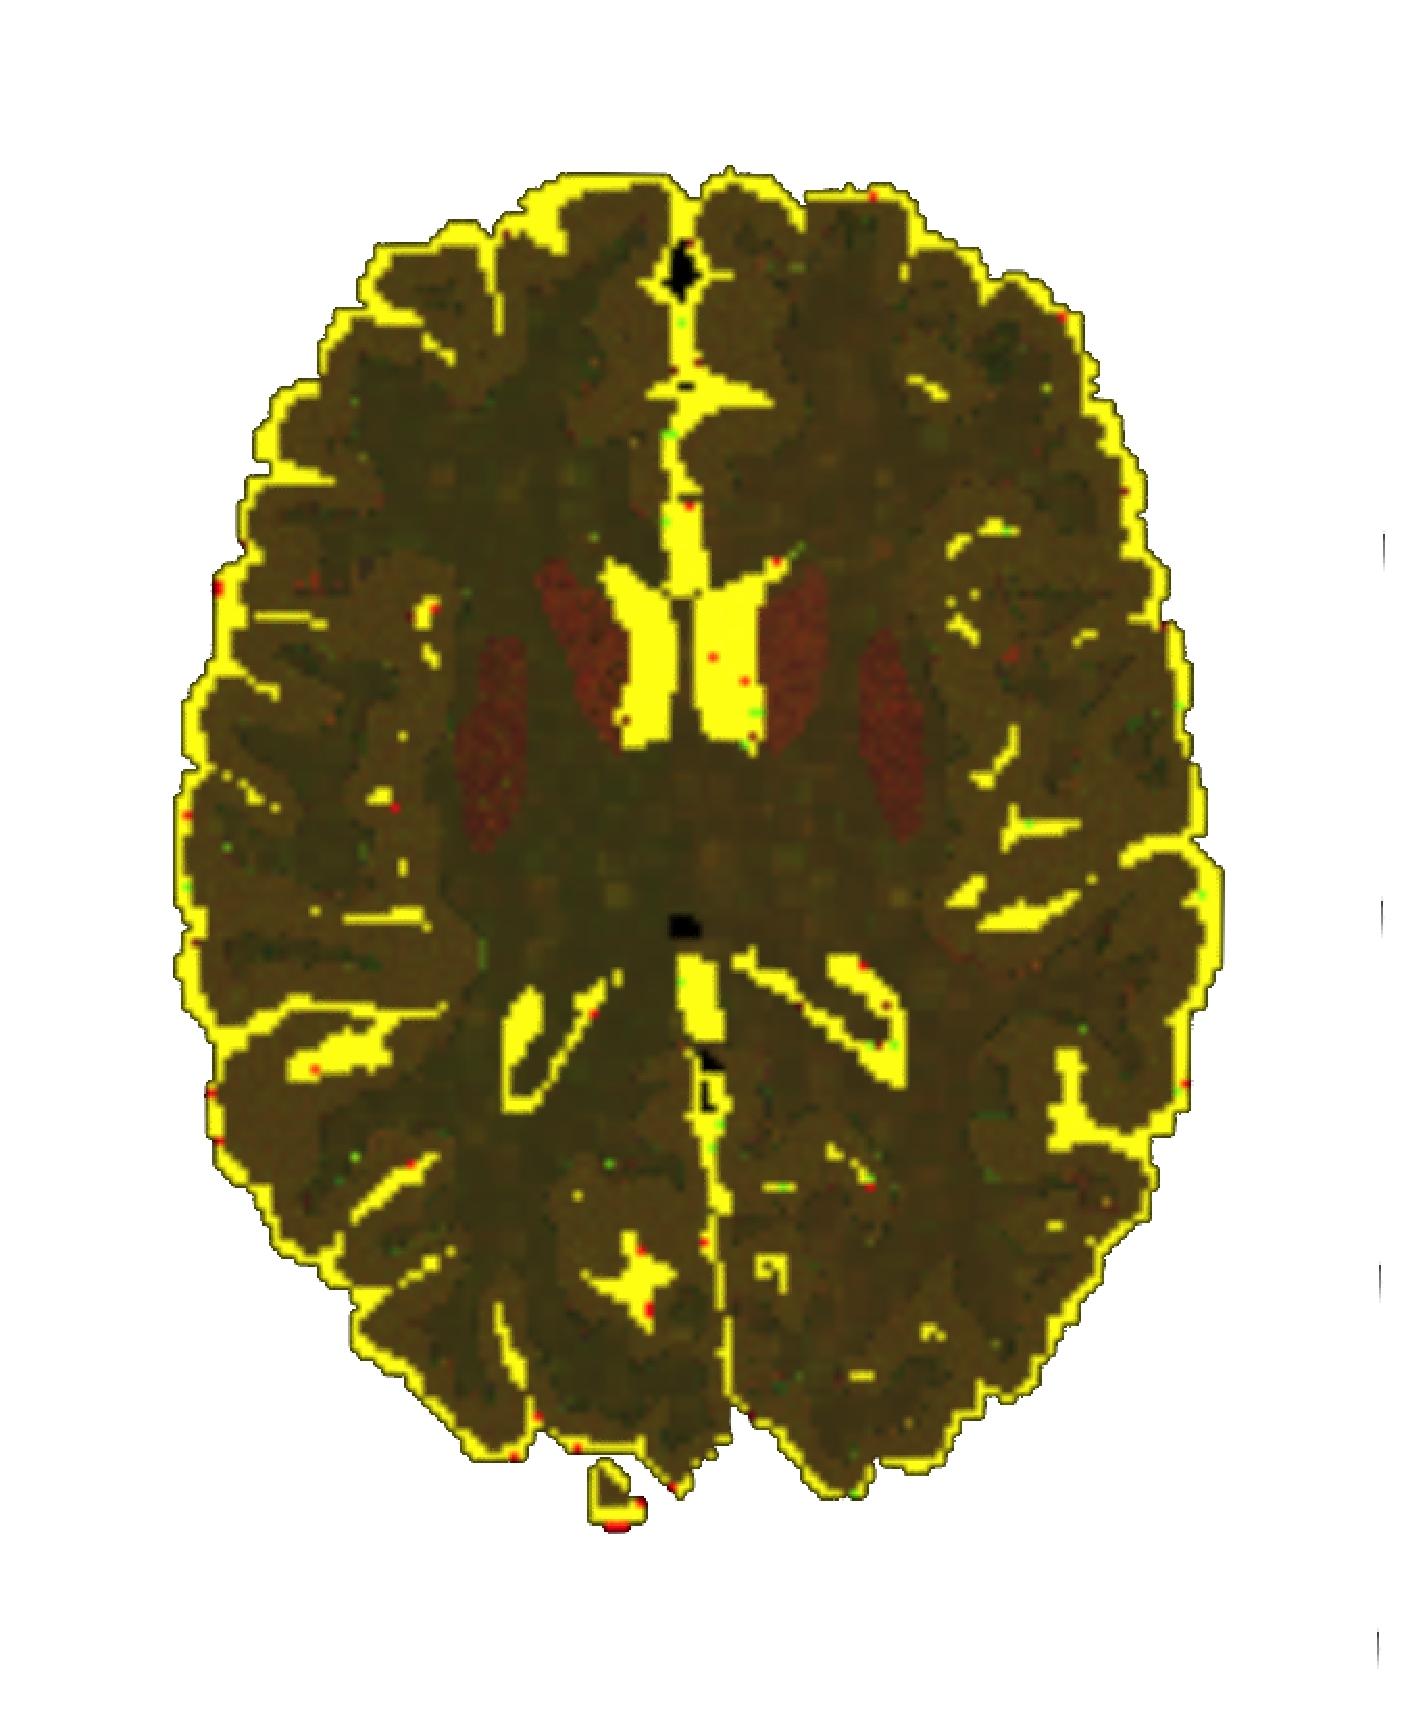
\epsfig{file = SynthPhysicalParameters1.eps, width =7cm}} 
\caption[Synthetic textured complex.]{The textured s-reps can generate an image of physical parameters by merging 
					the results into a single image.
					The WM and cerebral spinal fluid regions are textured 
					with the extended $X2U$ map of the cortex. Figures (a) to (c) show the results of merging 
					the solid textures into a single image. 
					$T1$ is shown in red, $T2$ in green and $M0$ in blue. 
					All channels are rescaled between $[0-255]$ for visualization purposes.
					}
 \label{fig:physicalParamsObjectsImage}  
\end{figure}
The following section evaluates the quality of the simulated images.

\section{Evaluation of the simulated image}
\label{sec:EvaluationSimulation}

To evaluate the quality of the images, a segmentation with \textit{Freesurfer} is performed. 
If these images are close enough to real MRI acquisitions, they should be able to be segmented by
\textit{Freesurfer}. Figure \ref{fig:physicalParamsObjectsImageSimu} shows the result of the simulation with \textit{SimuBloch}.
The simulation parameters of the acquisition were $TR=500$ and $TE=8.4$.

\begin{figure} 
 \centering   
 \subfigure[Subject 1]{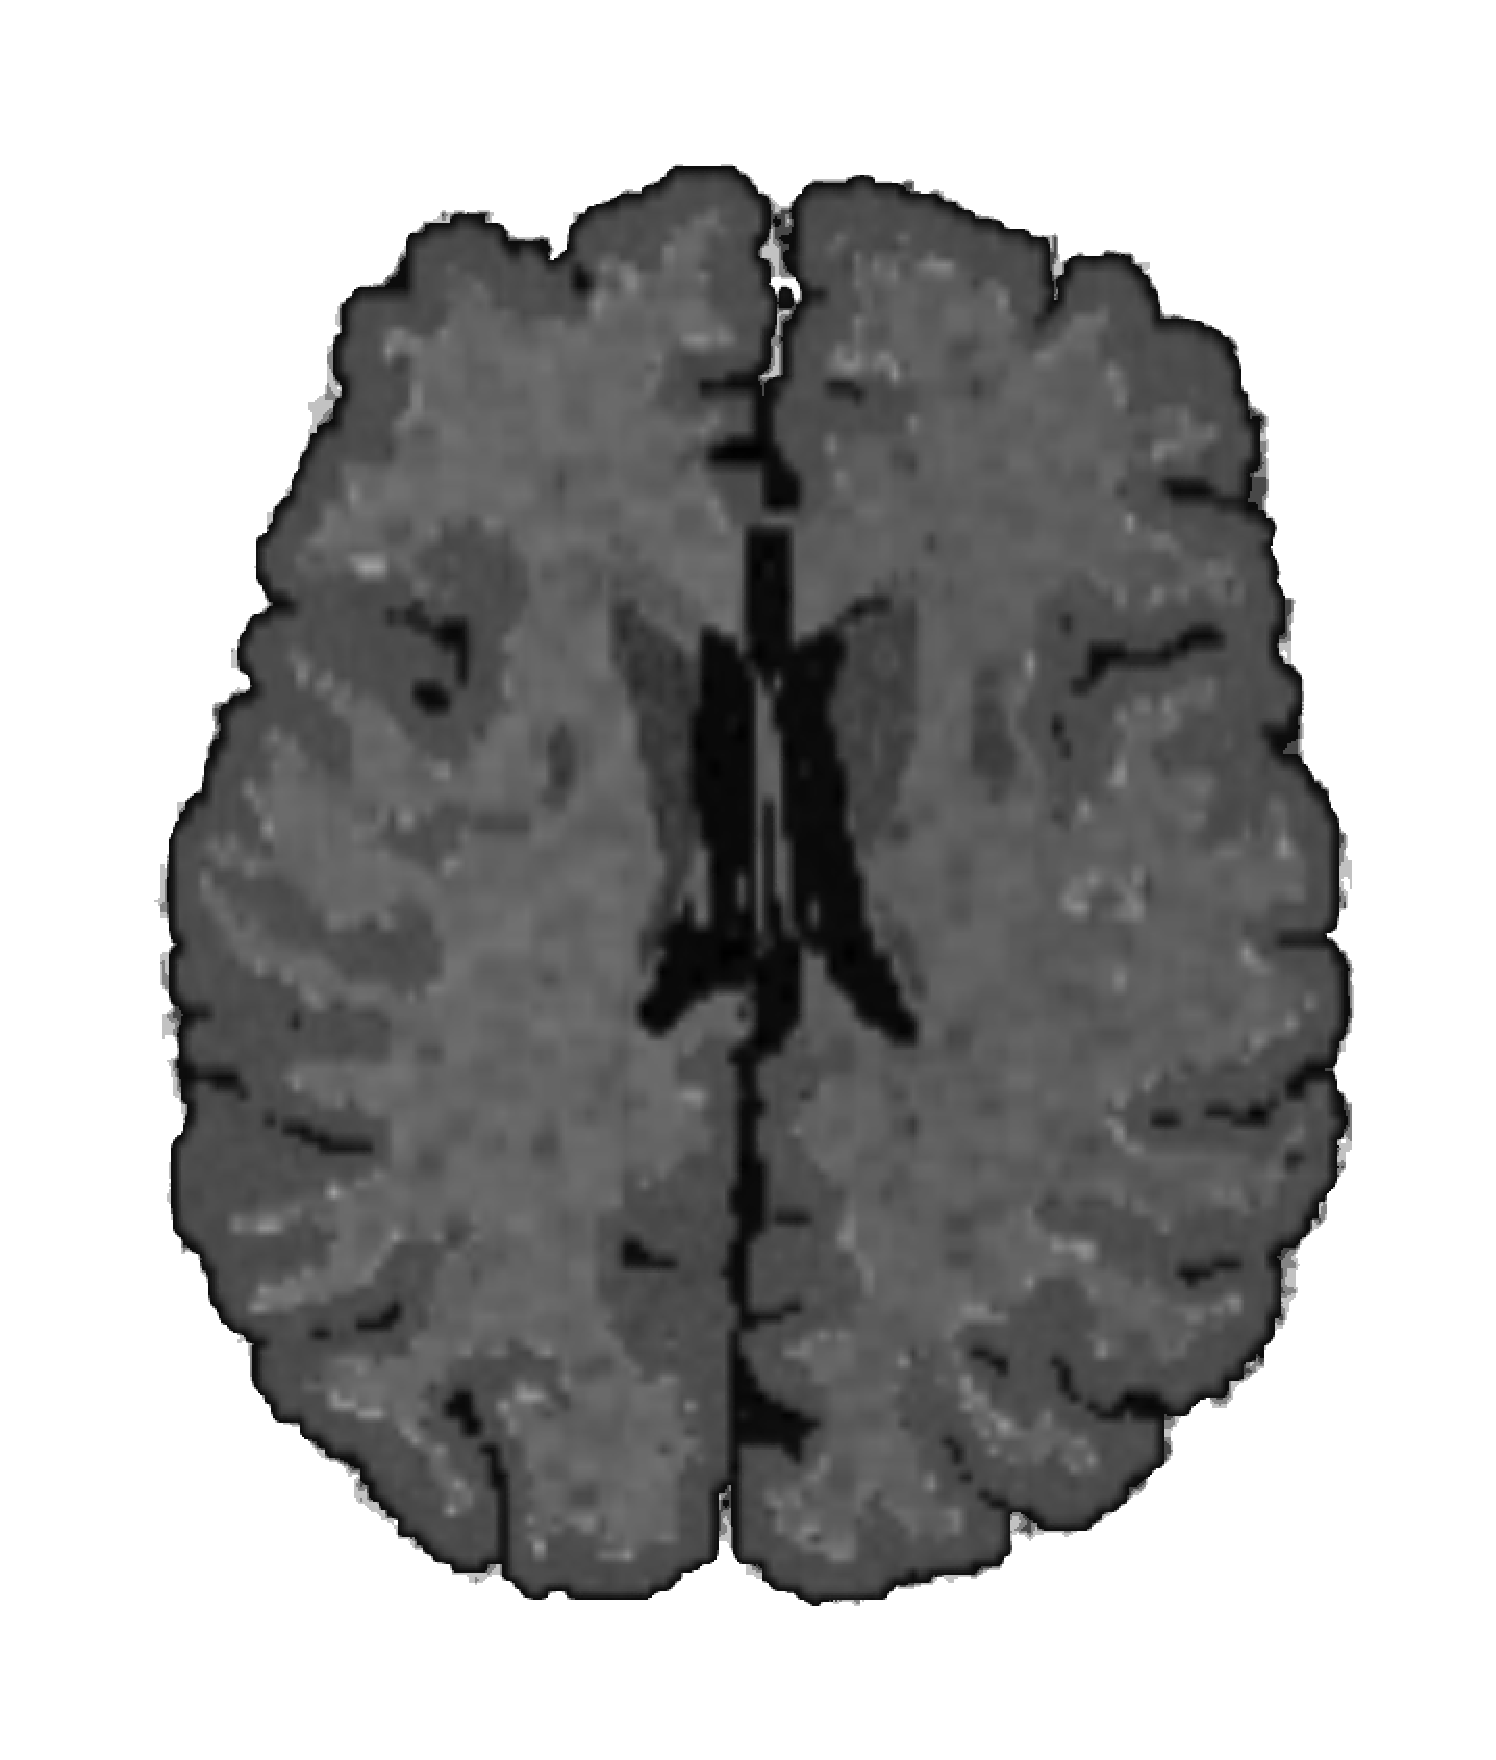
\epsfig{file = SynthSimulated.eps, width =7cm}}
 \subfigure[Subject 2]{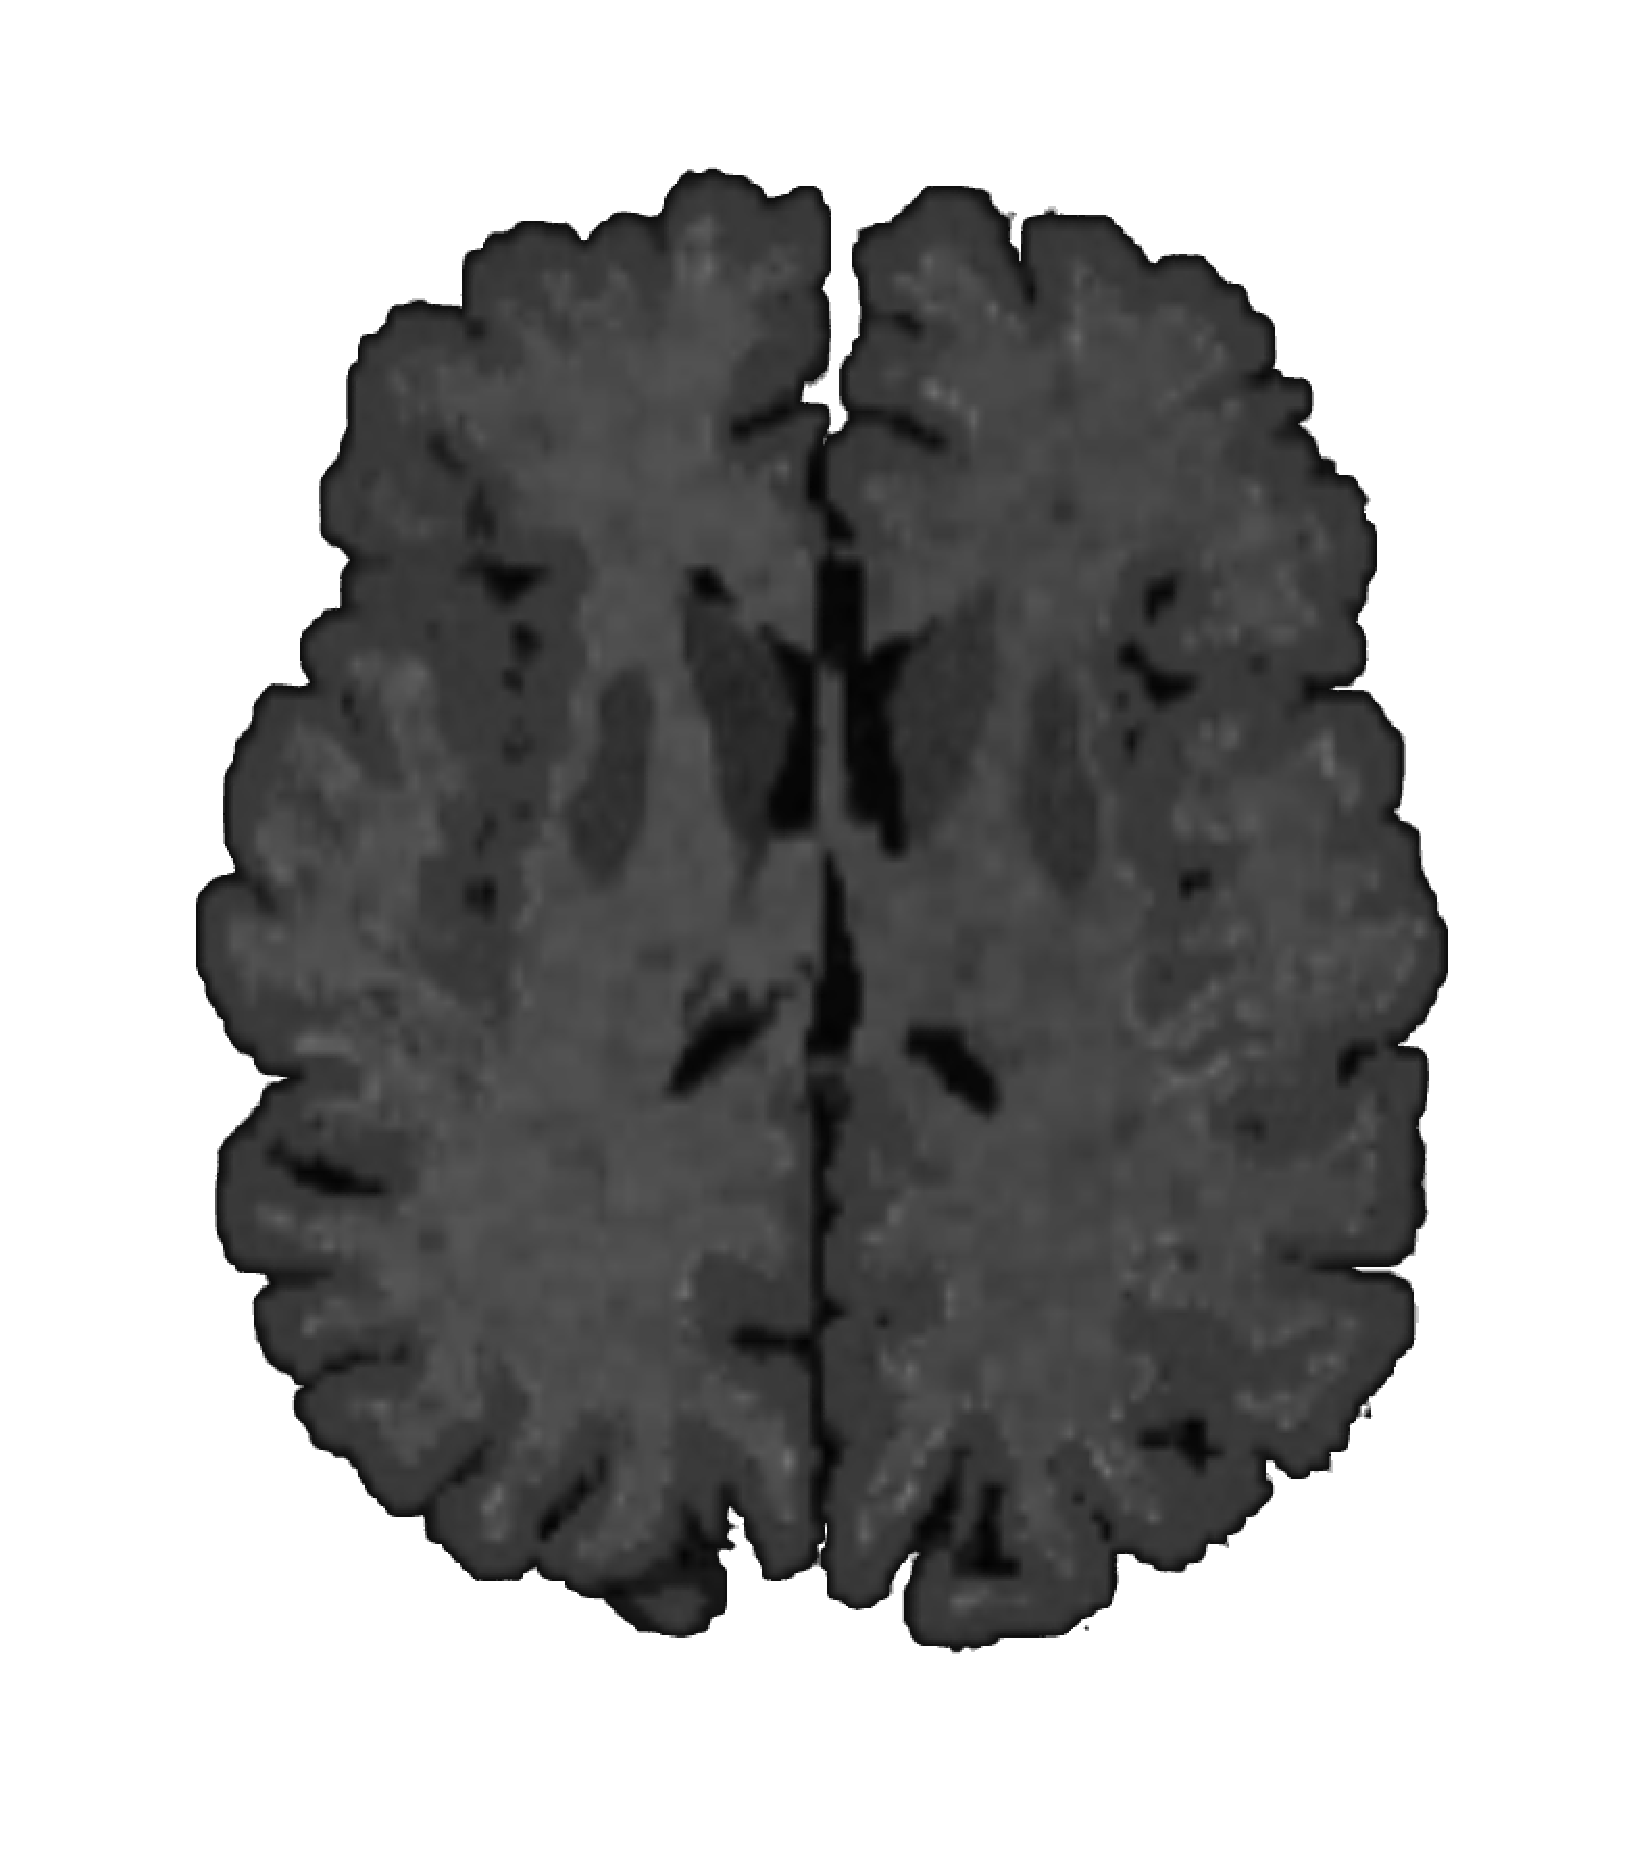
\epsfig{file = SynthSimulated0.eps, width =7cm}}
 \subfigure[Subject 3]{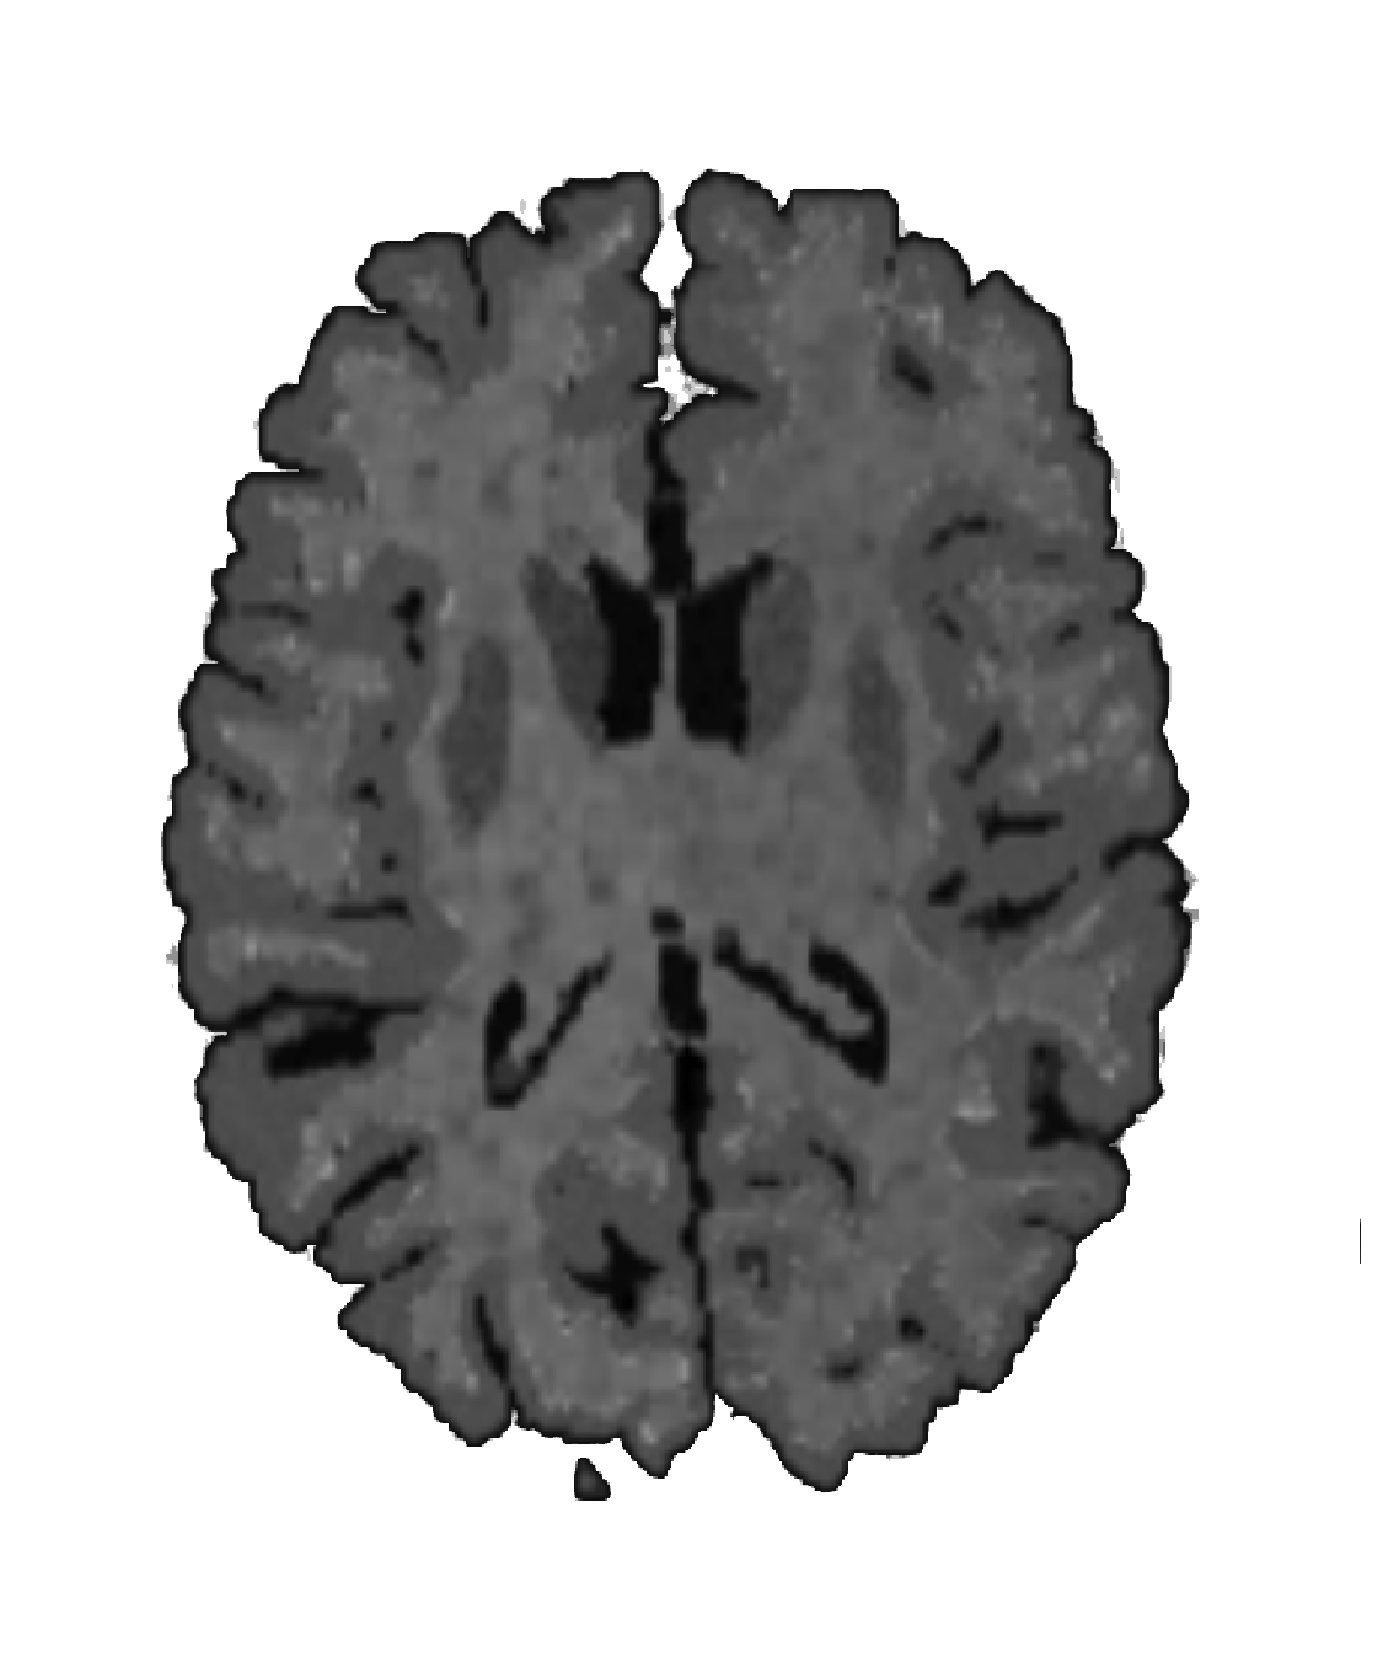
\epsfig{file = SynthSimulated1.eps, width =7cm}} 
\caption[Simulated brain MRI for three subjects.]{Result of \textit{SimuBloch} using the physical parameters image shown in Figure \ref{fig:physicalParamsObjectsImage}.}
 \label{fig:physicalParamsObjectsImageSimu}  
\end{figure}

\begin{figure} 
 \centering   
 \subfigure[Subject 1]{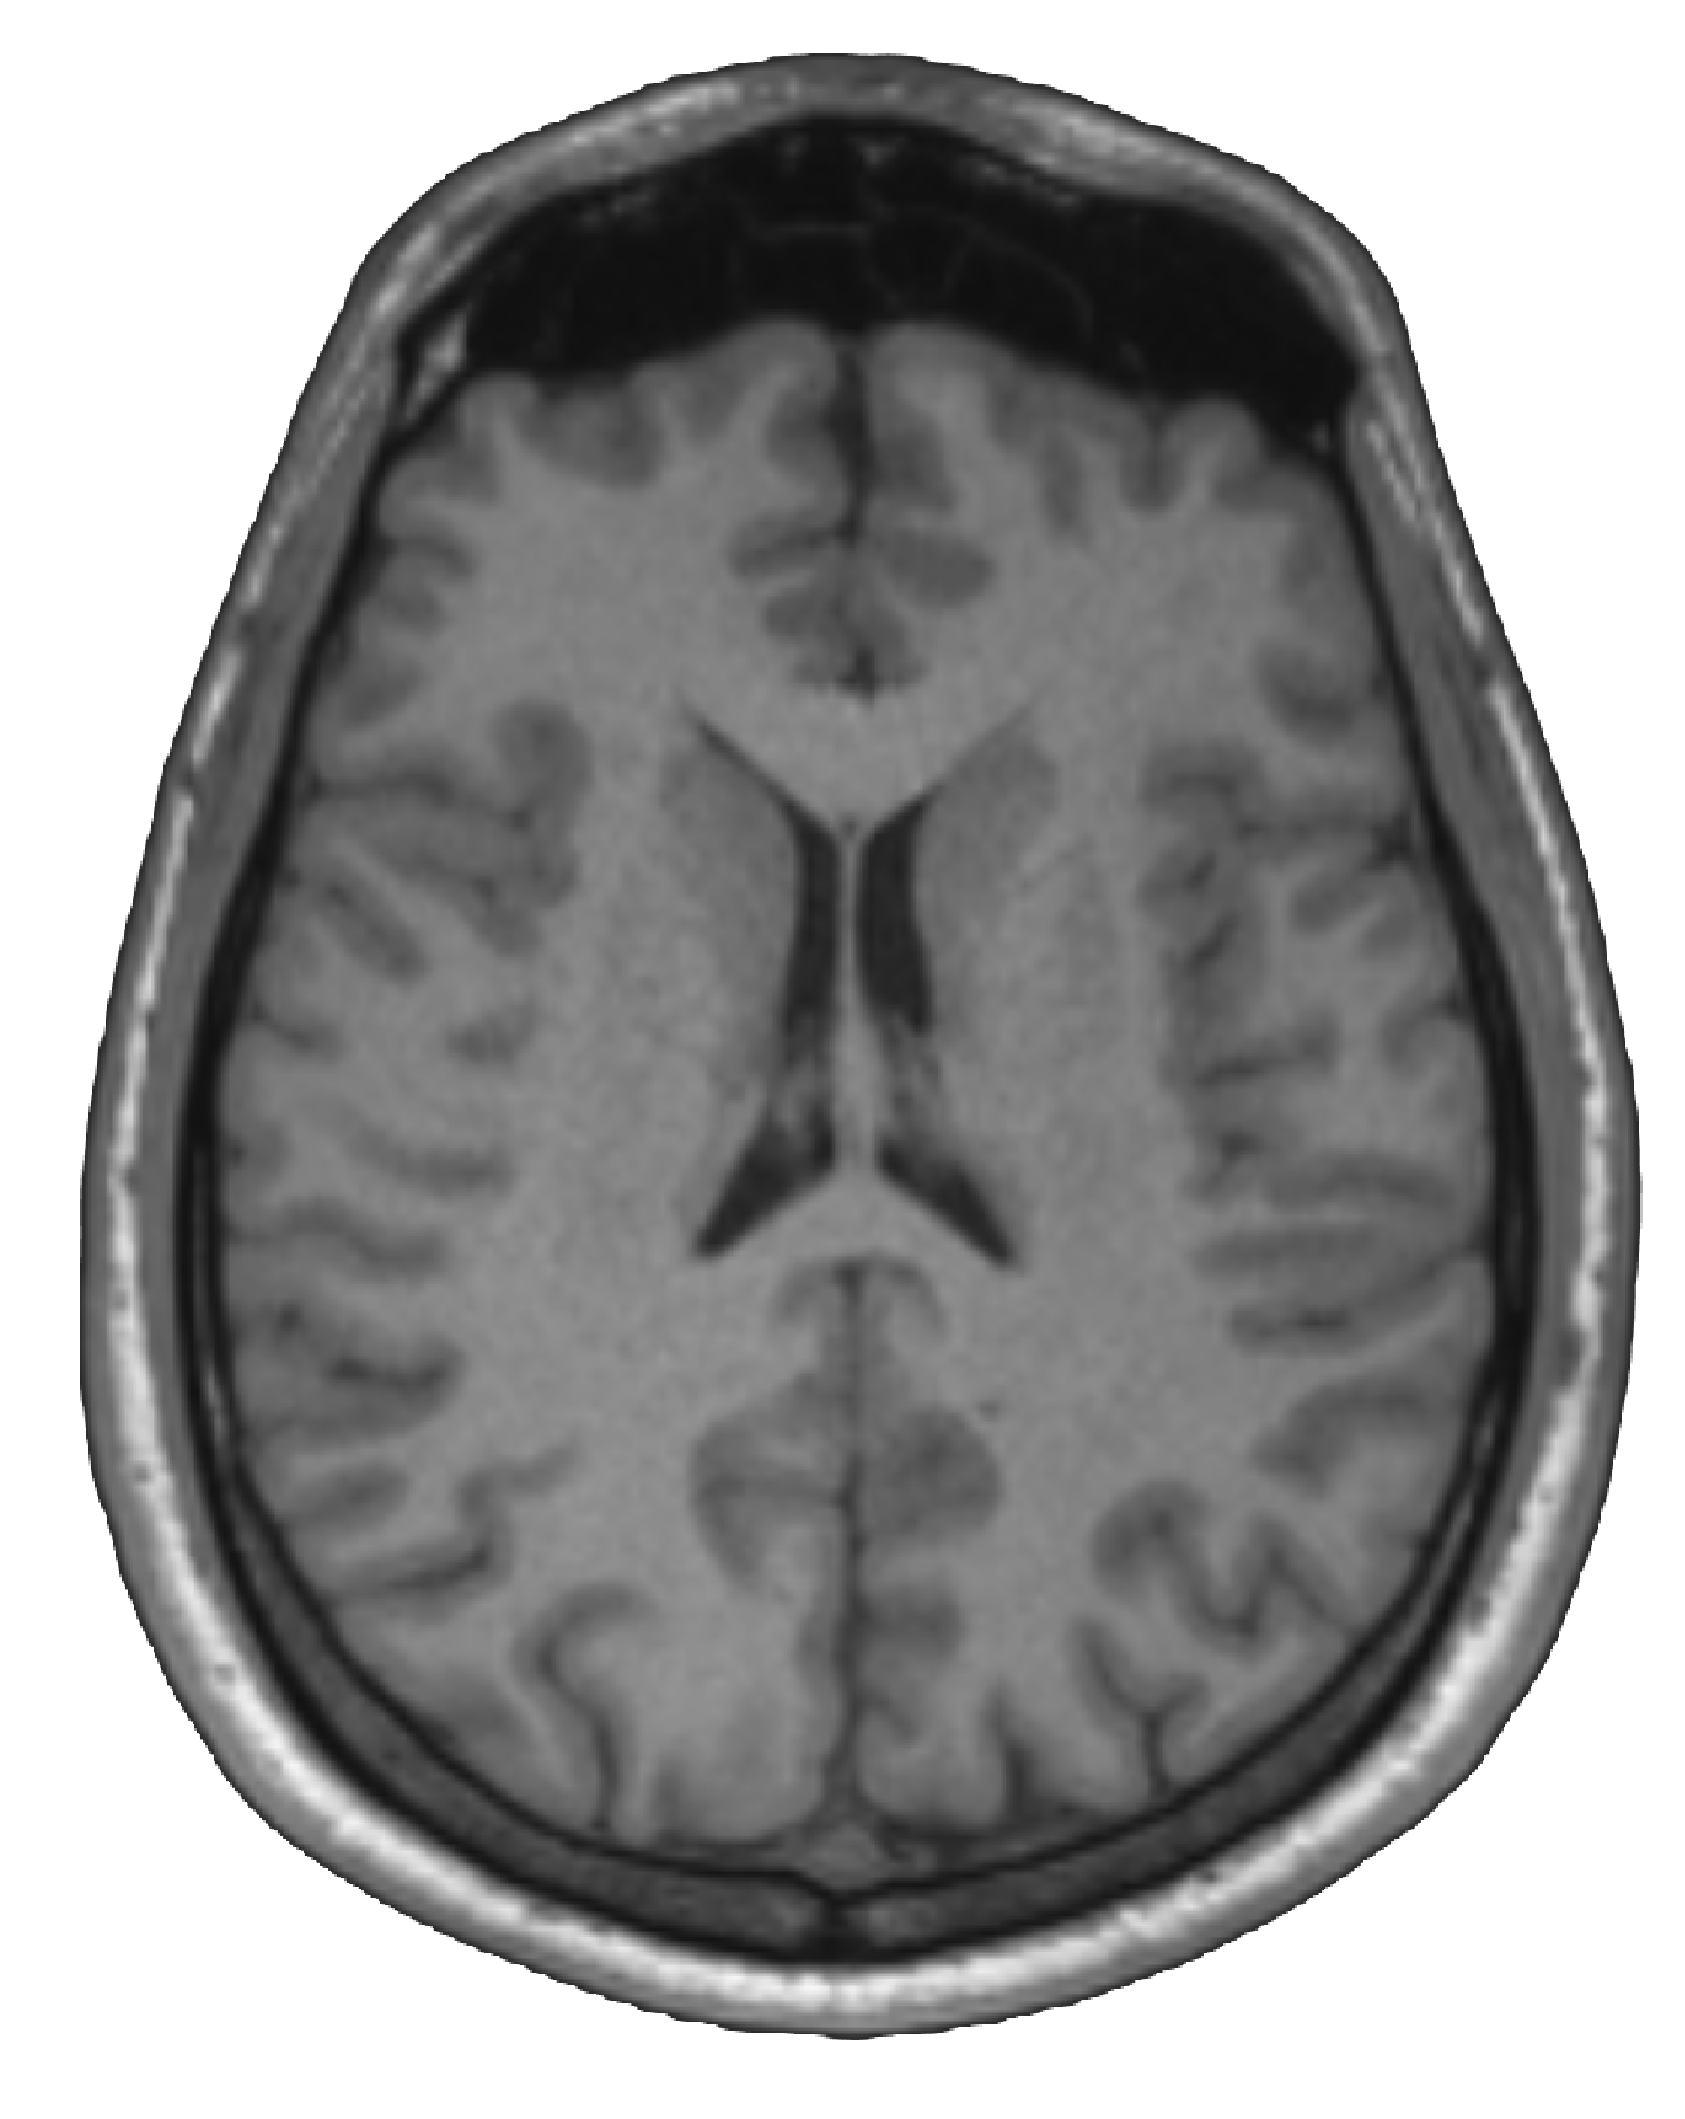
\epsfig{file = SynthOrig.eps, width =7cm}}
 \subfigure[Subject 2]{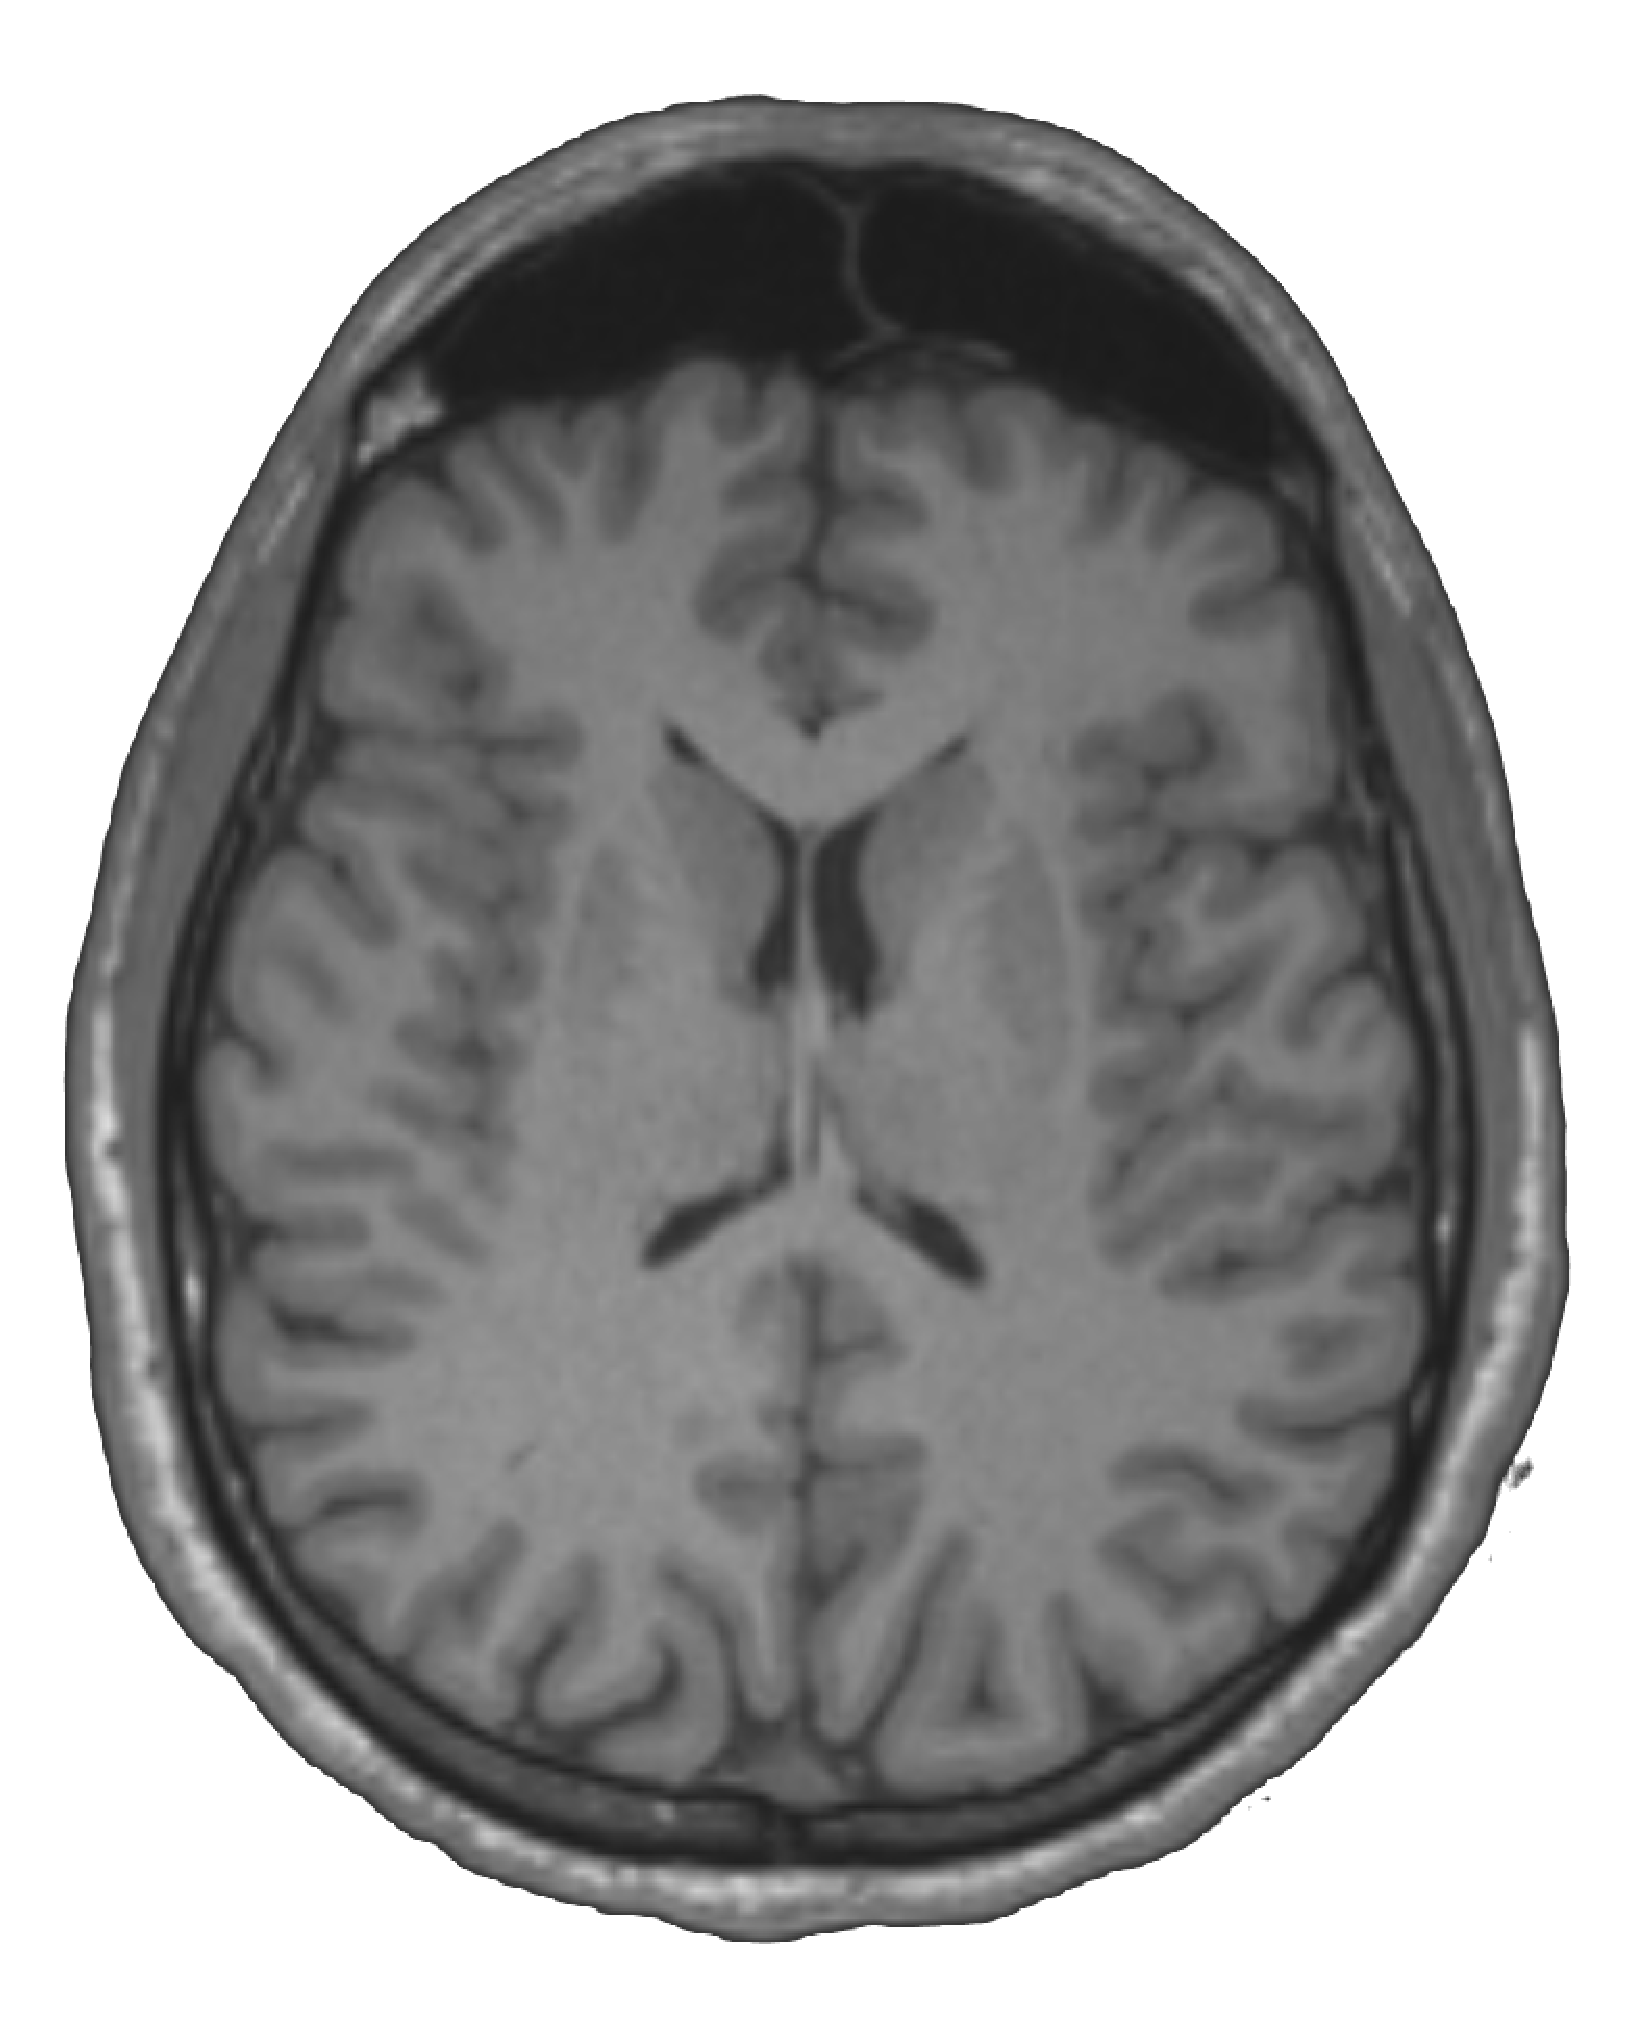
\epsfig{file = SynthOrig0.eps, width =7cm}}
 \subfigure[Subject 3]{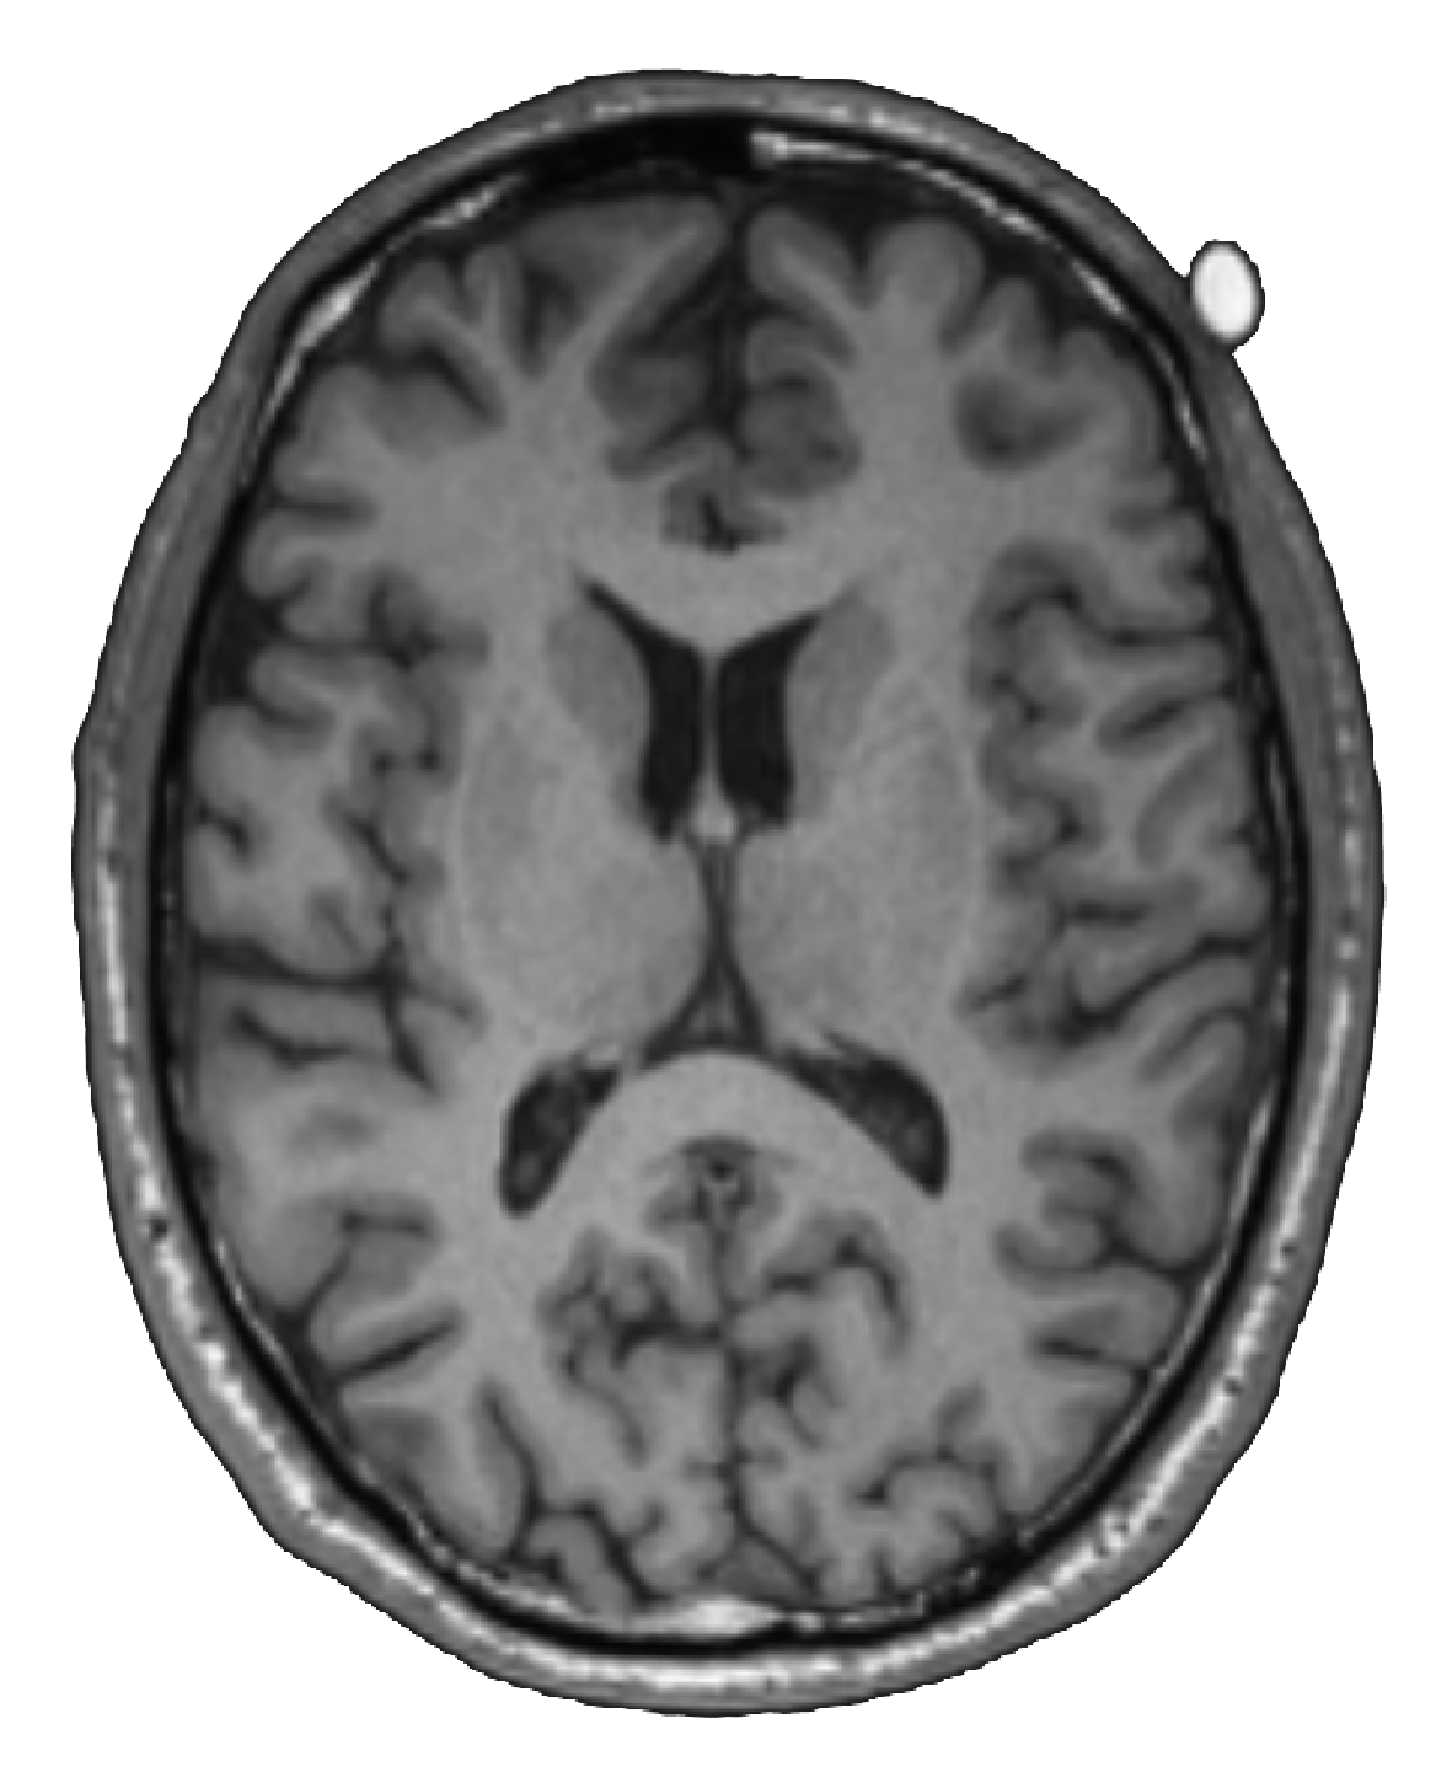
\epsfig{file = SynthOrig1.eps, width =7cm}} 
\caption[Original brain MRI for three subjects.]{The source images used to create the s-rep models. The slices resemble those shown in Figure \ref{fig:physicalParamsObjectsImageSimu}, i.e., the simulated images.}
 \label{fig:physicalParamsObjectsImageOrig}  
\end{figure}

As expected, \textit{Freesurfer} is able to segment the images and produces a cortical parcellation and subcortical labeling of structures.
The results of the segmentation are shown in Figure \ref{fig:physicalParamsObjectsSegmentedImage}.
The image shows the WM and GM surfaces in yellow and cyan respectively;
the labels given to the subcortical structures; and the cortical parcellation.
\begin{figure} 
 \centering   
 \subfigure[Subject 1]{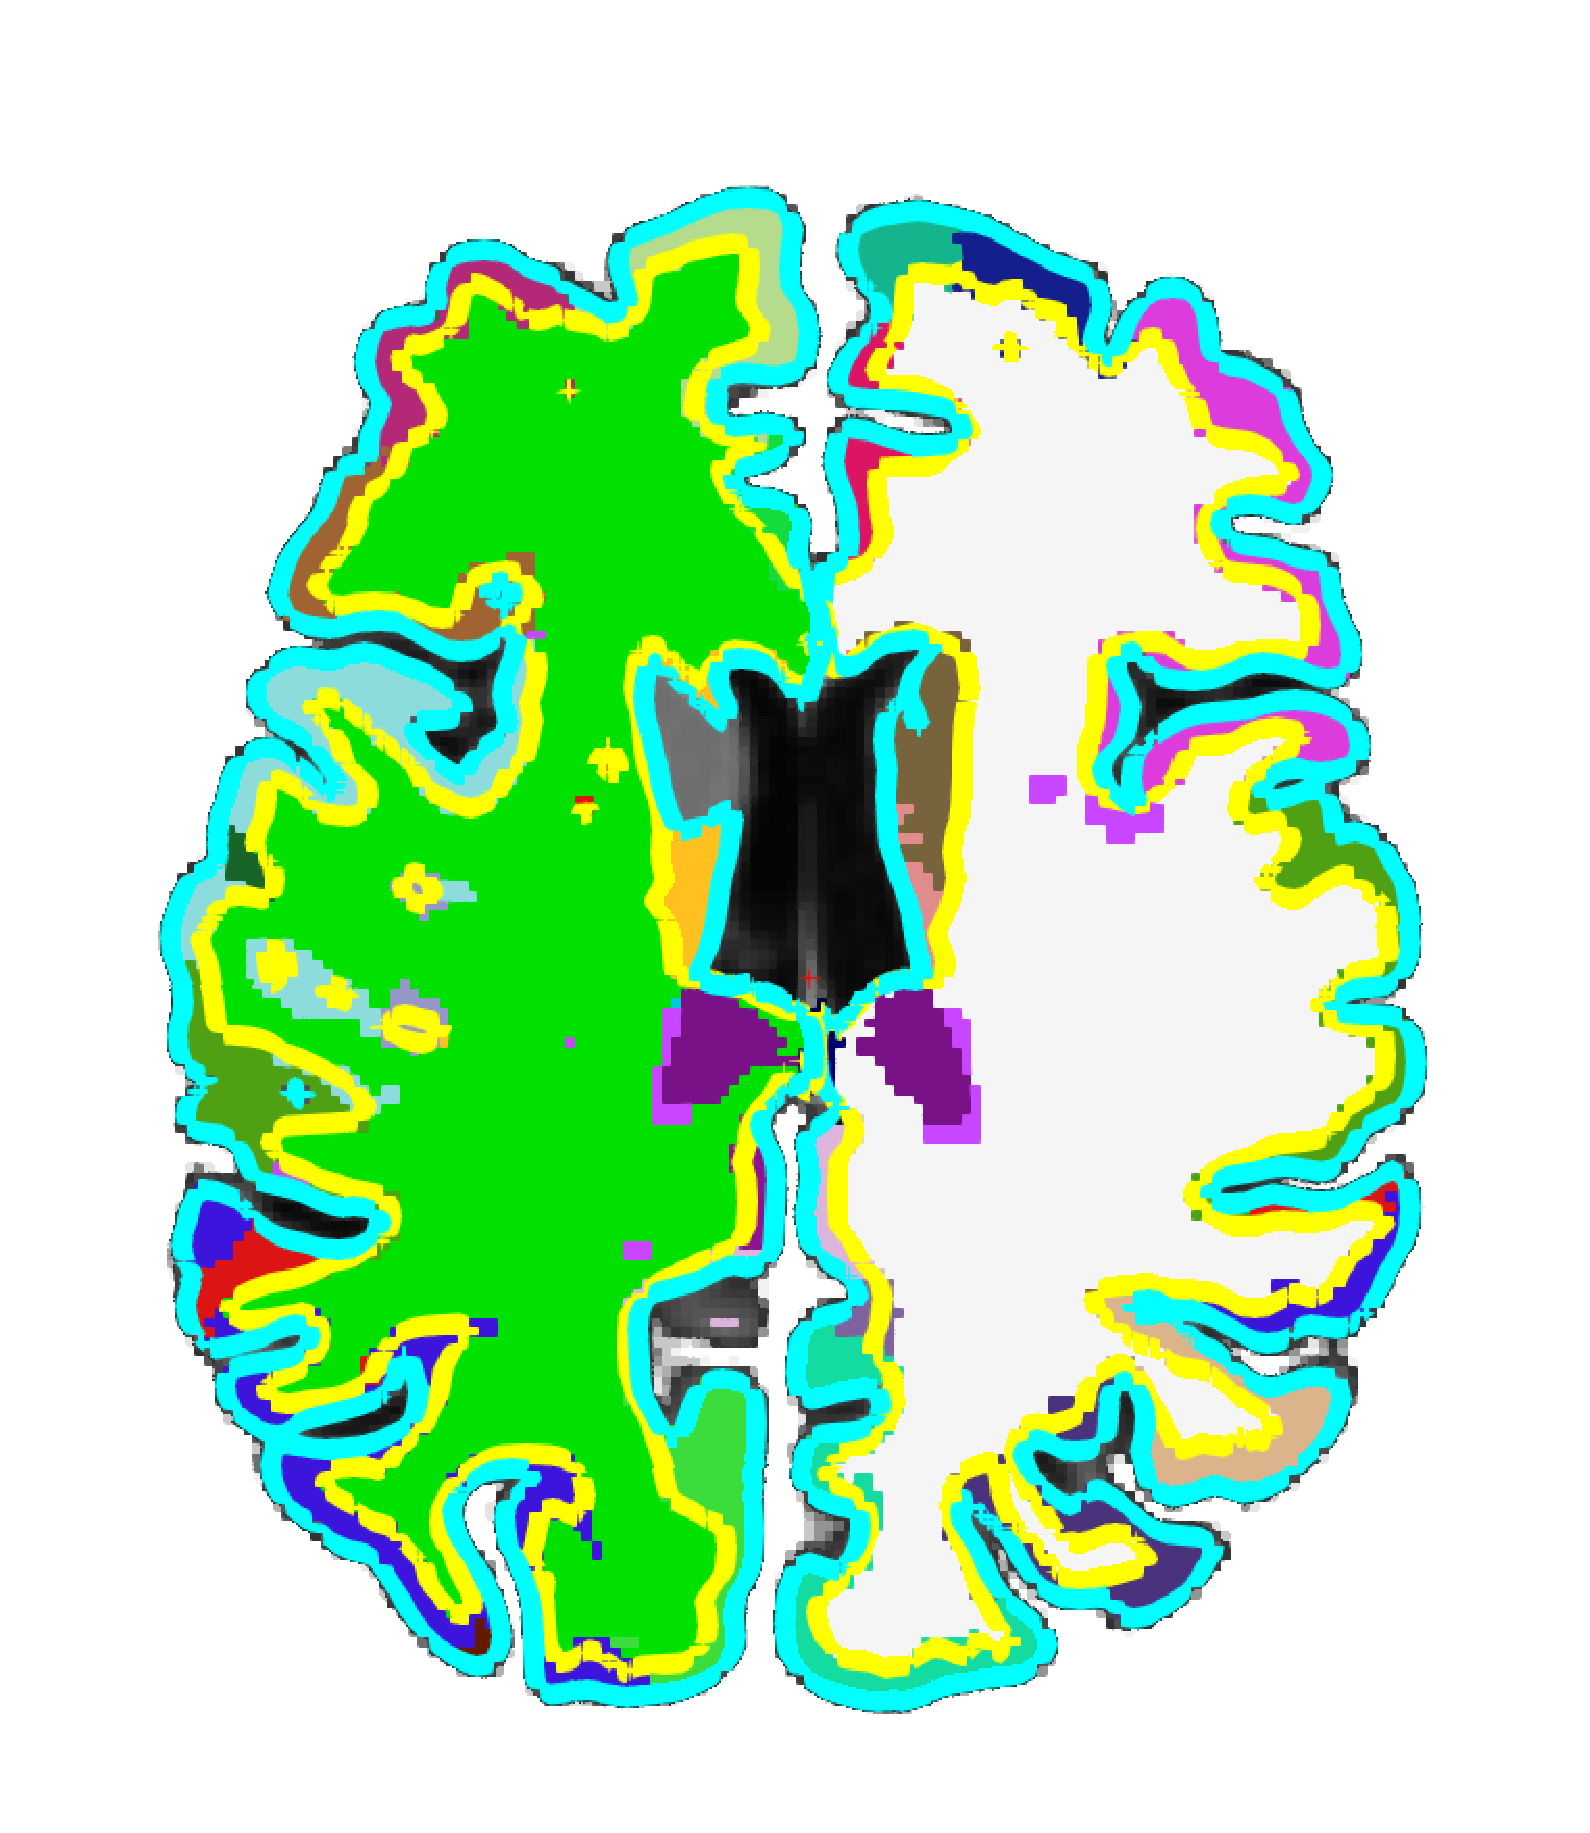
\epsfig{file = SynthSegmented.eps, width =7cm}}
 \subfigure[Subject 2]{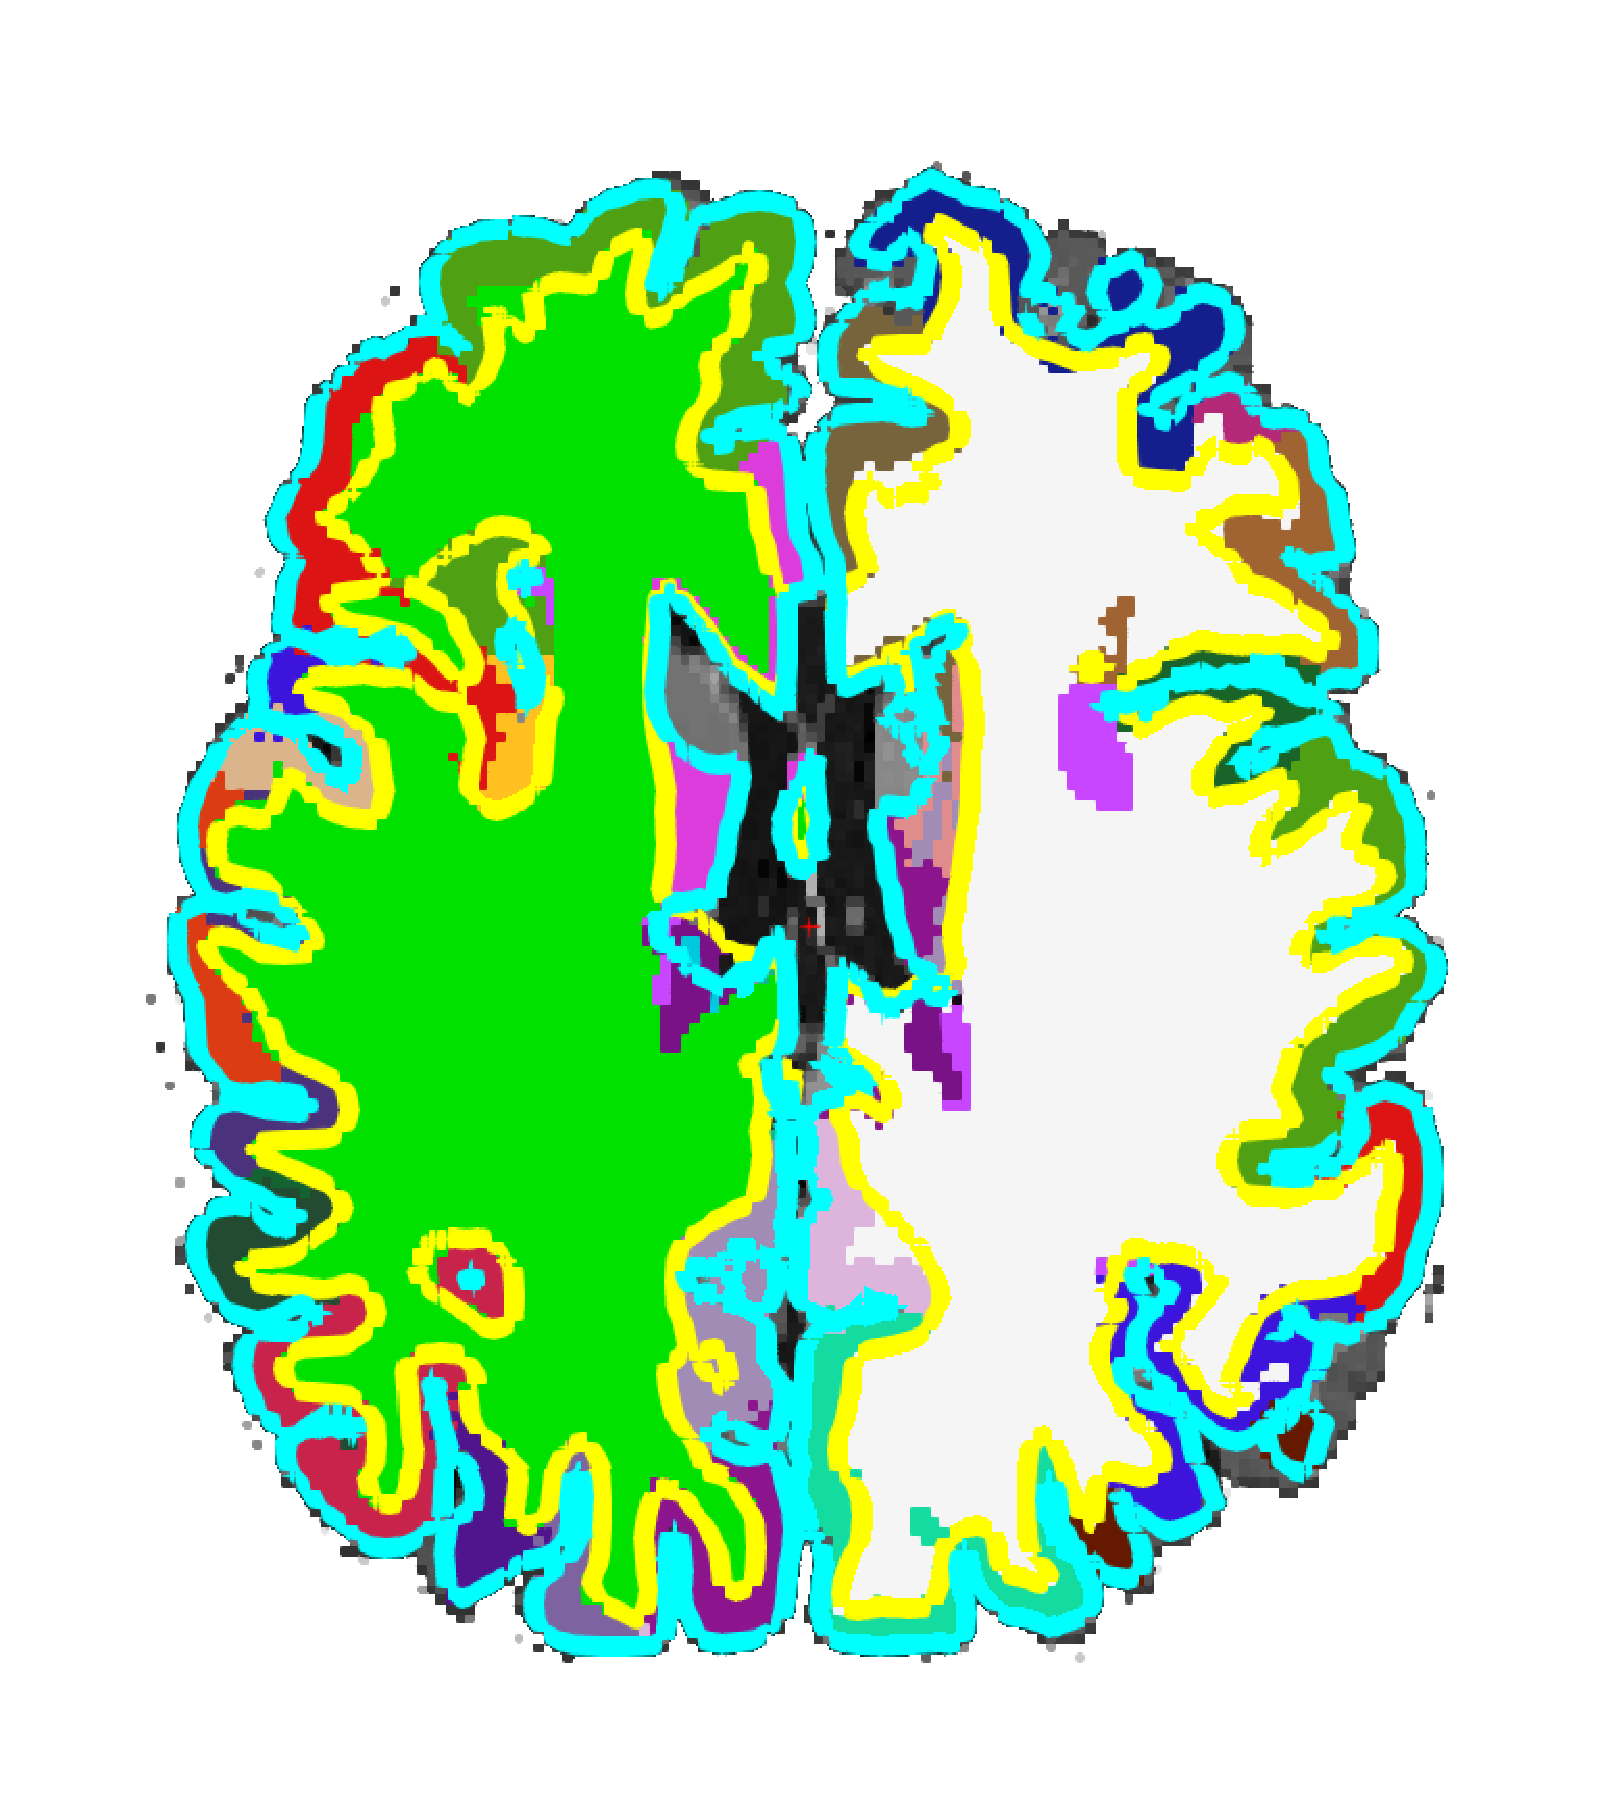
\epsfig{file = SynthSegmented0.eps, width =7cm}}
 \subfigure[Subject 3]{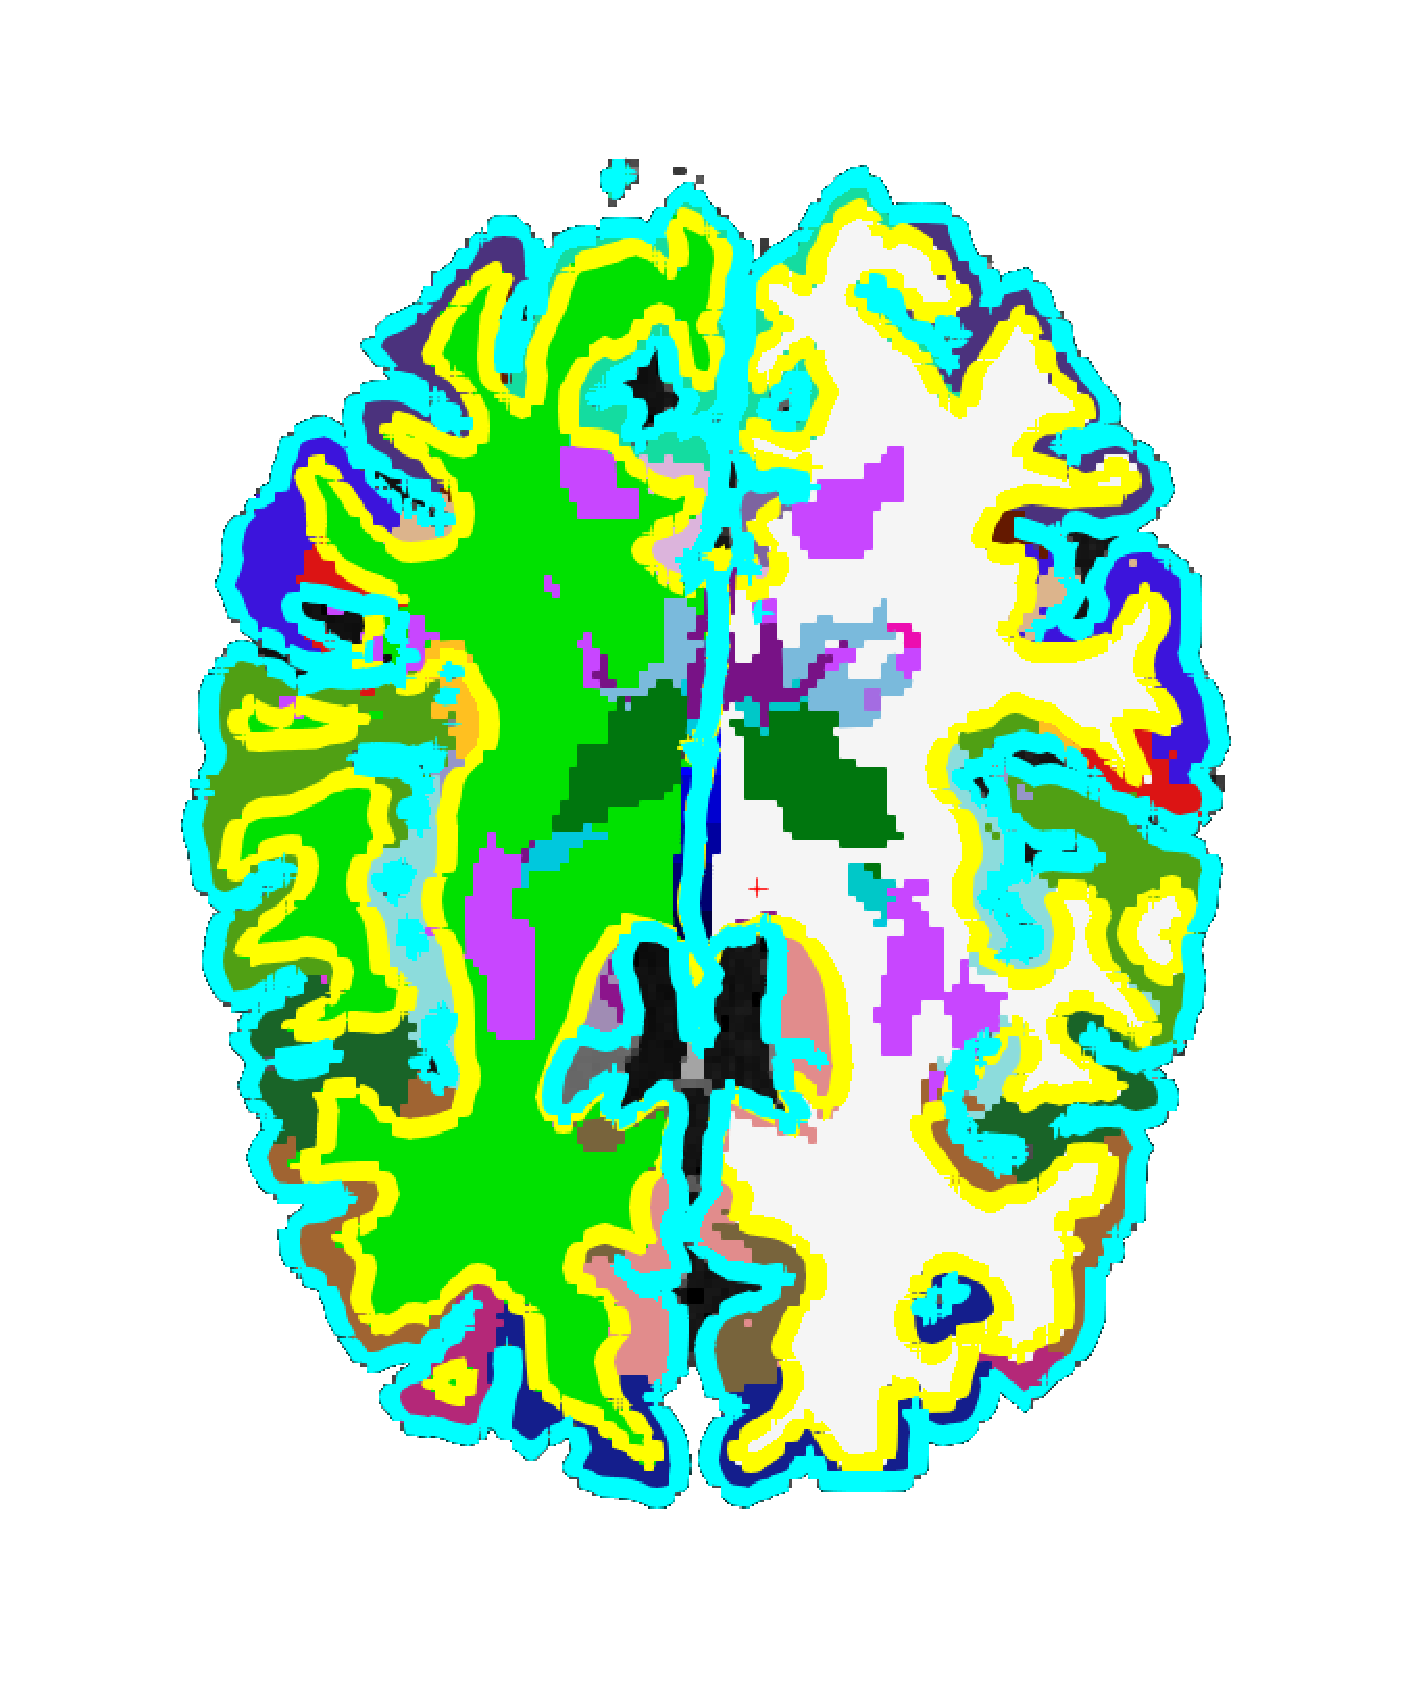
\epsfig{file = SynthSegmented1.eps, width =7cm}} 
\caption[Segmented MRI for three simulated subjects.]{Result of \textit{Freesurfer}. Freeview (a visualization tool from \textit{Freesurfer}) is used to 
							visualize the surfaces and the segmented labels of the subcortical structures.
							The yellow line corresponds to the WM surface and the red line to the GM surface.}
 \label{fig:physicalParamsObjectsSegmentedImage}  
\end{figure}

\begin{figure} 
 \centering   
 \subfigure[Left hemisphere WM surface.]{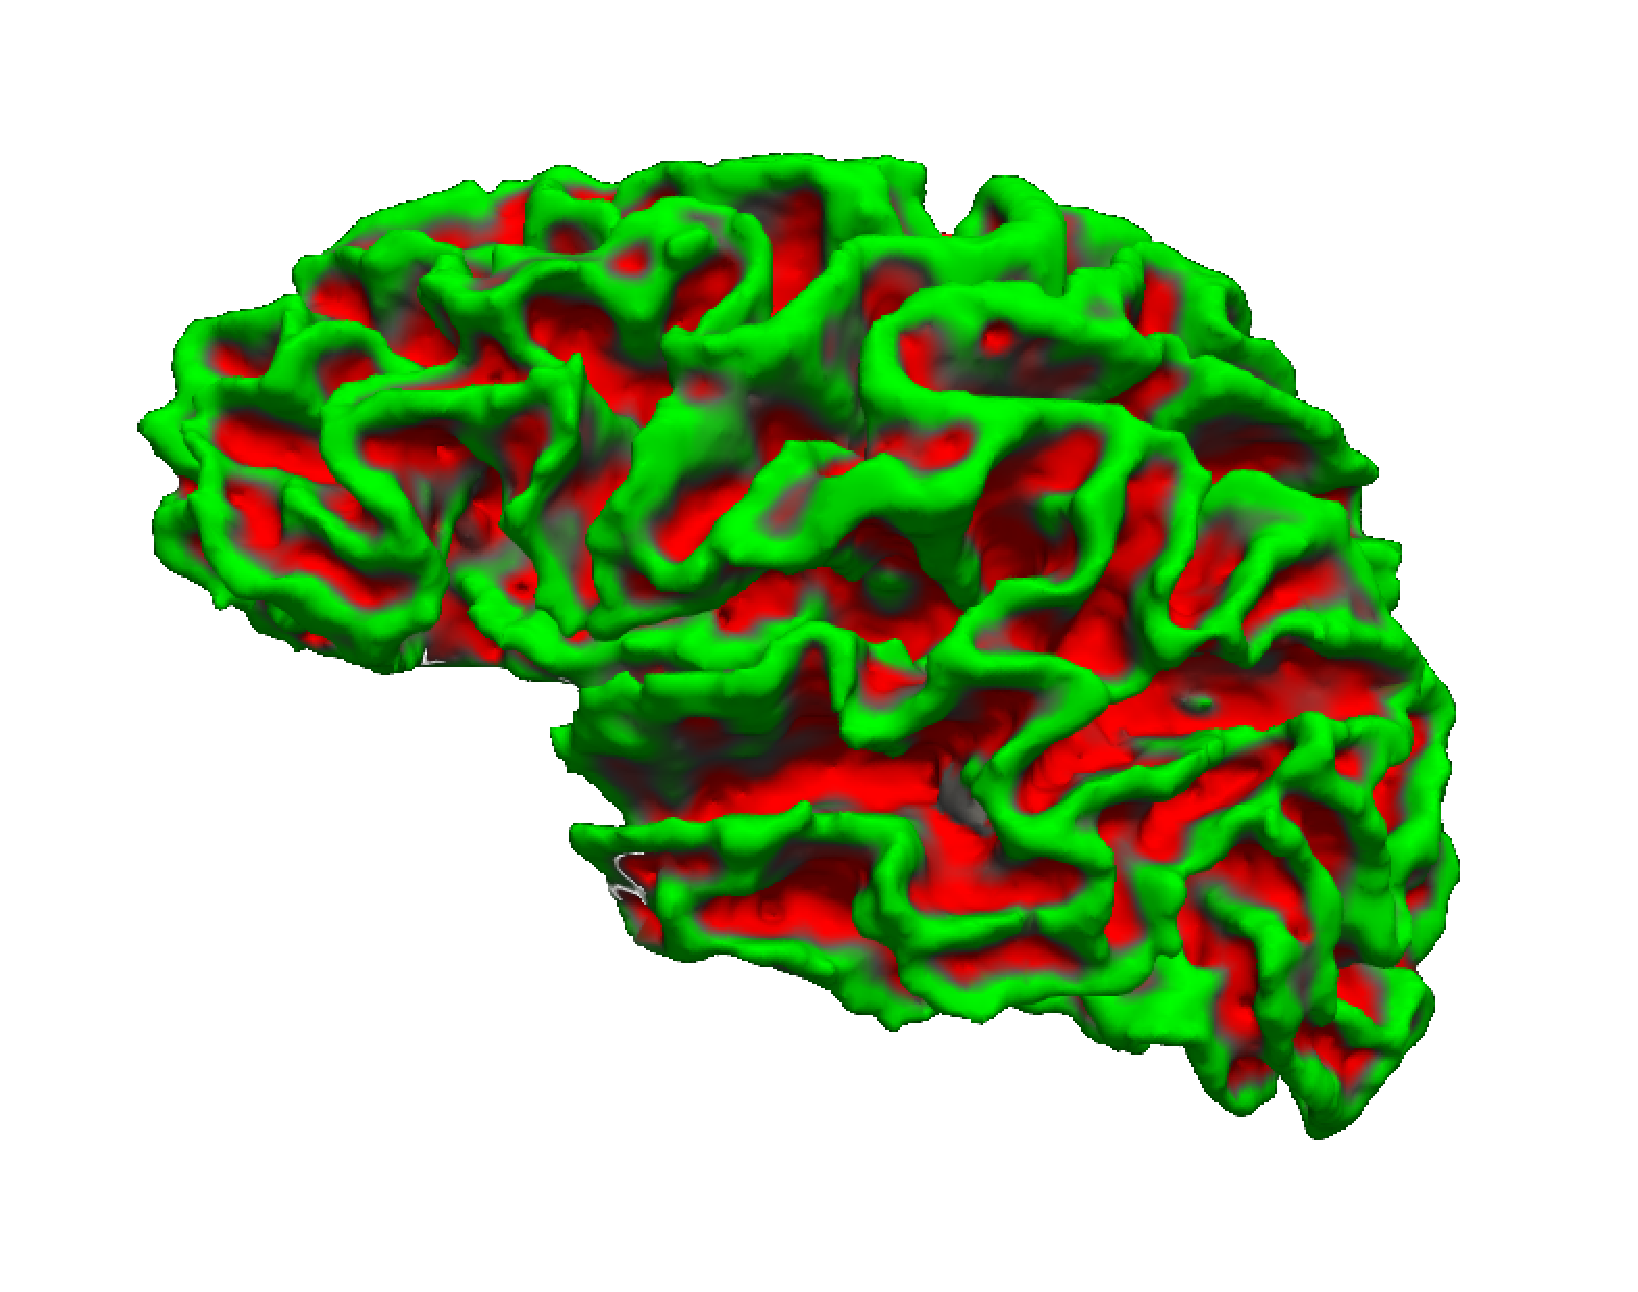
\epsfig{file = lh_S1_Simu_OrigSurface.eps, width =5.5cm} 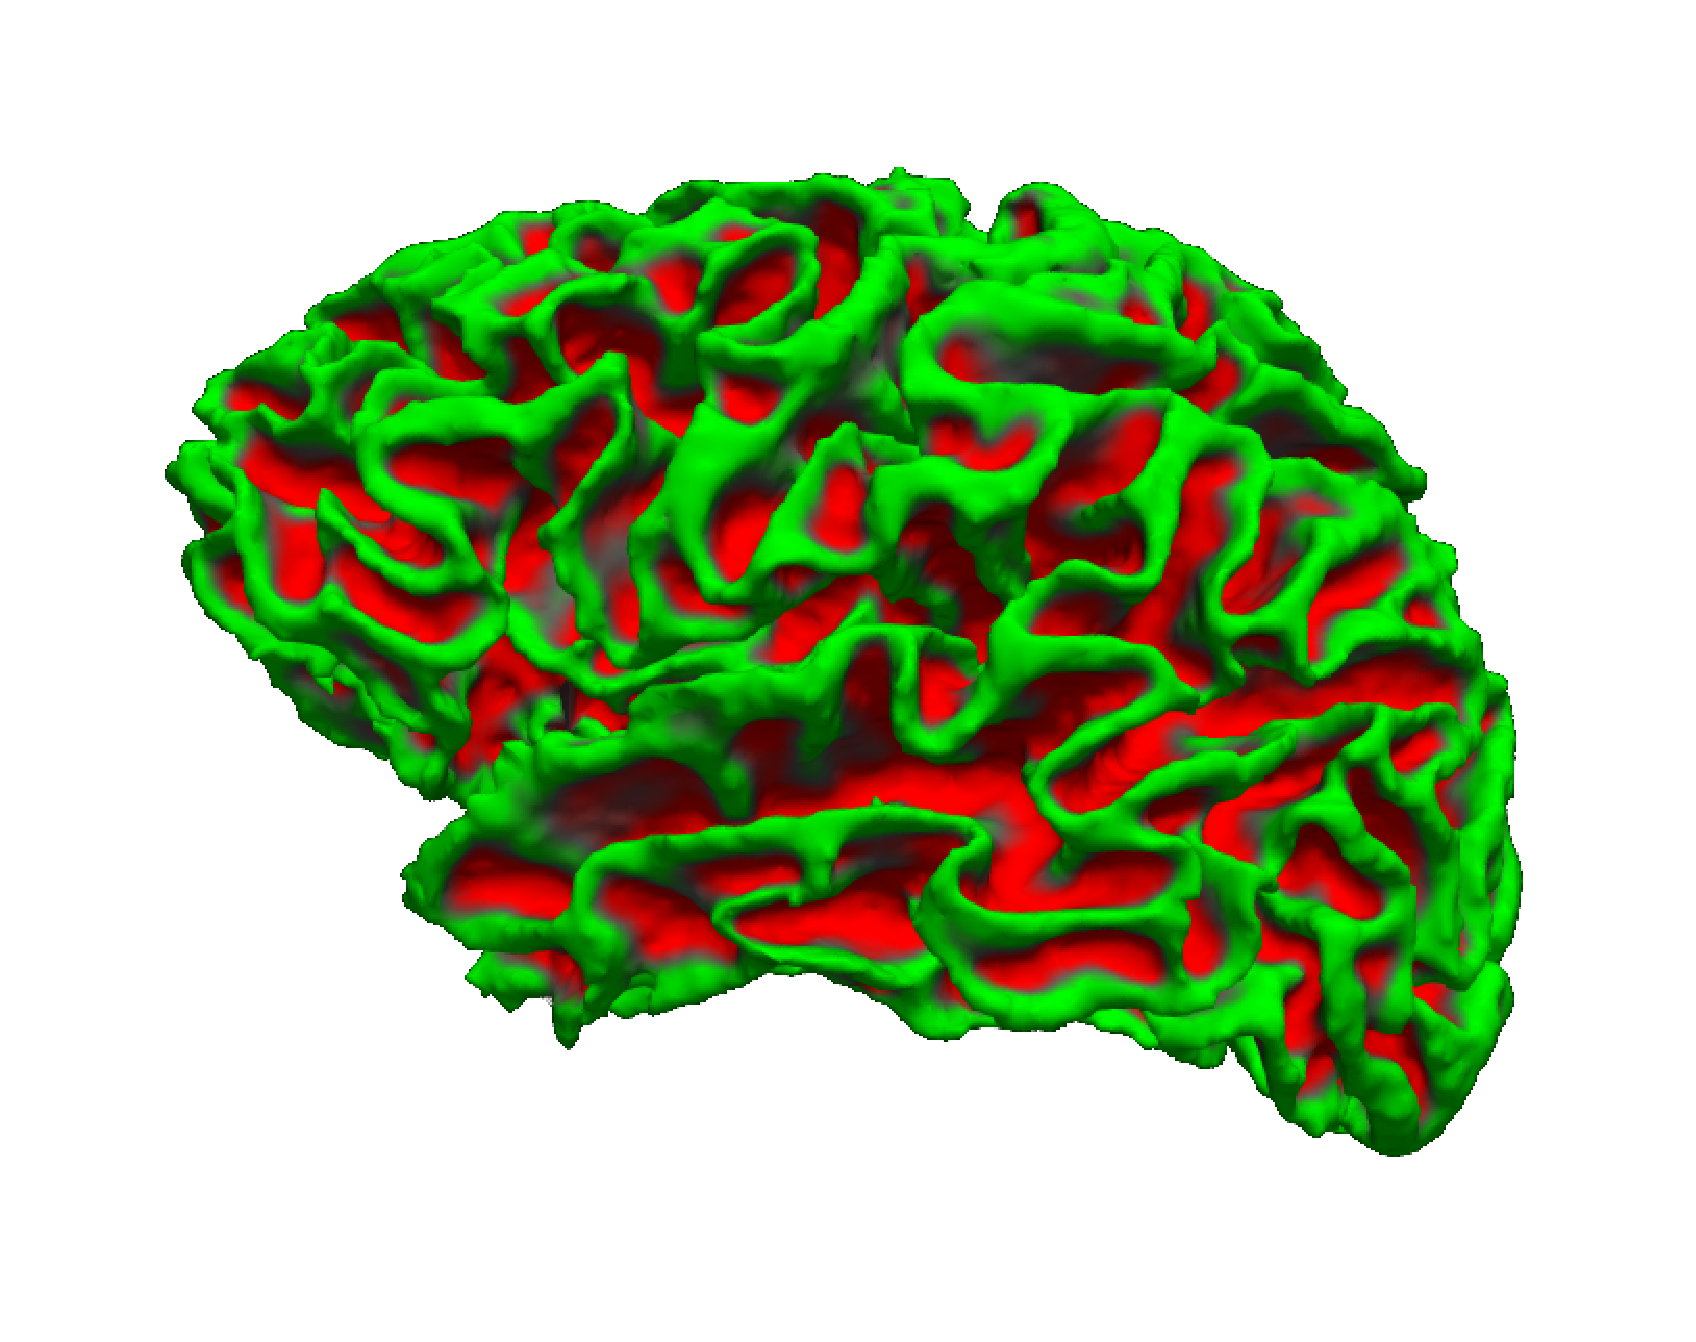
\epsfig{file = lh_S1_Orig_OrigSurface.eps, width =5.5cm}} 
 \subfigure[Left hemisphere GM surface.]{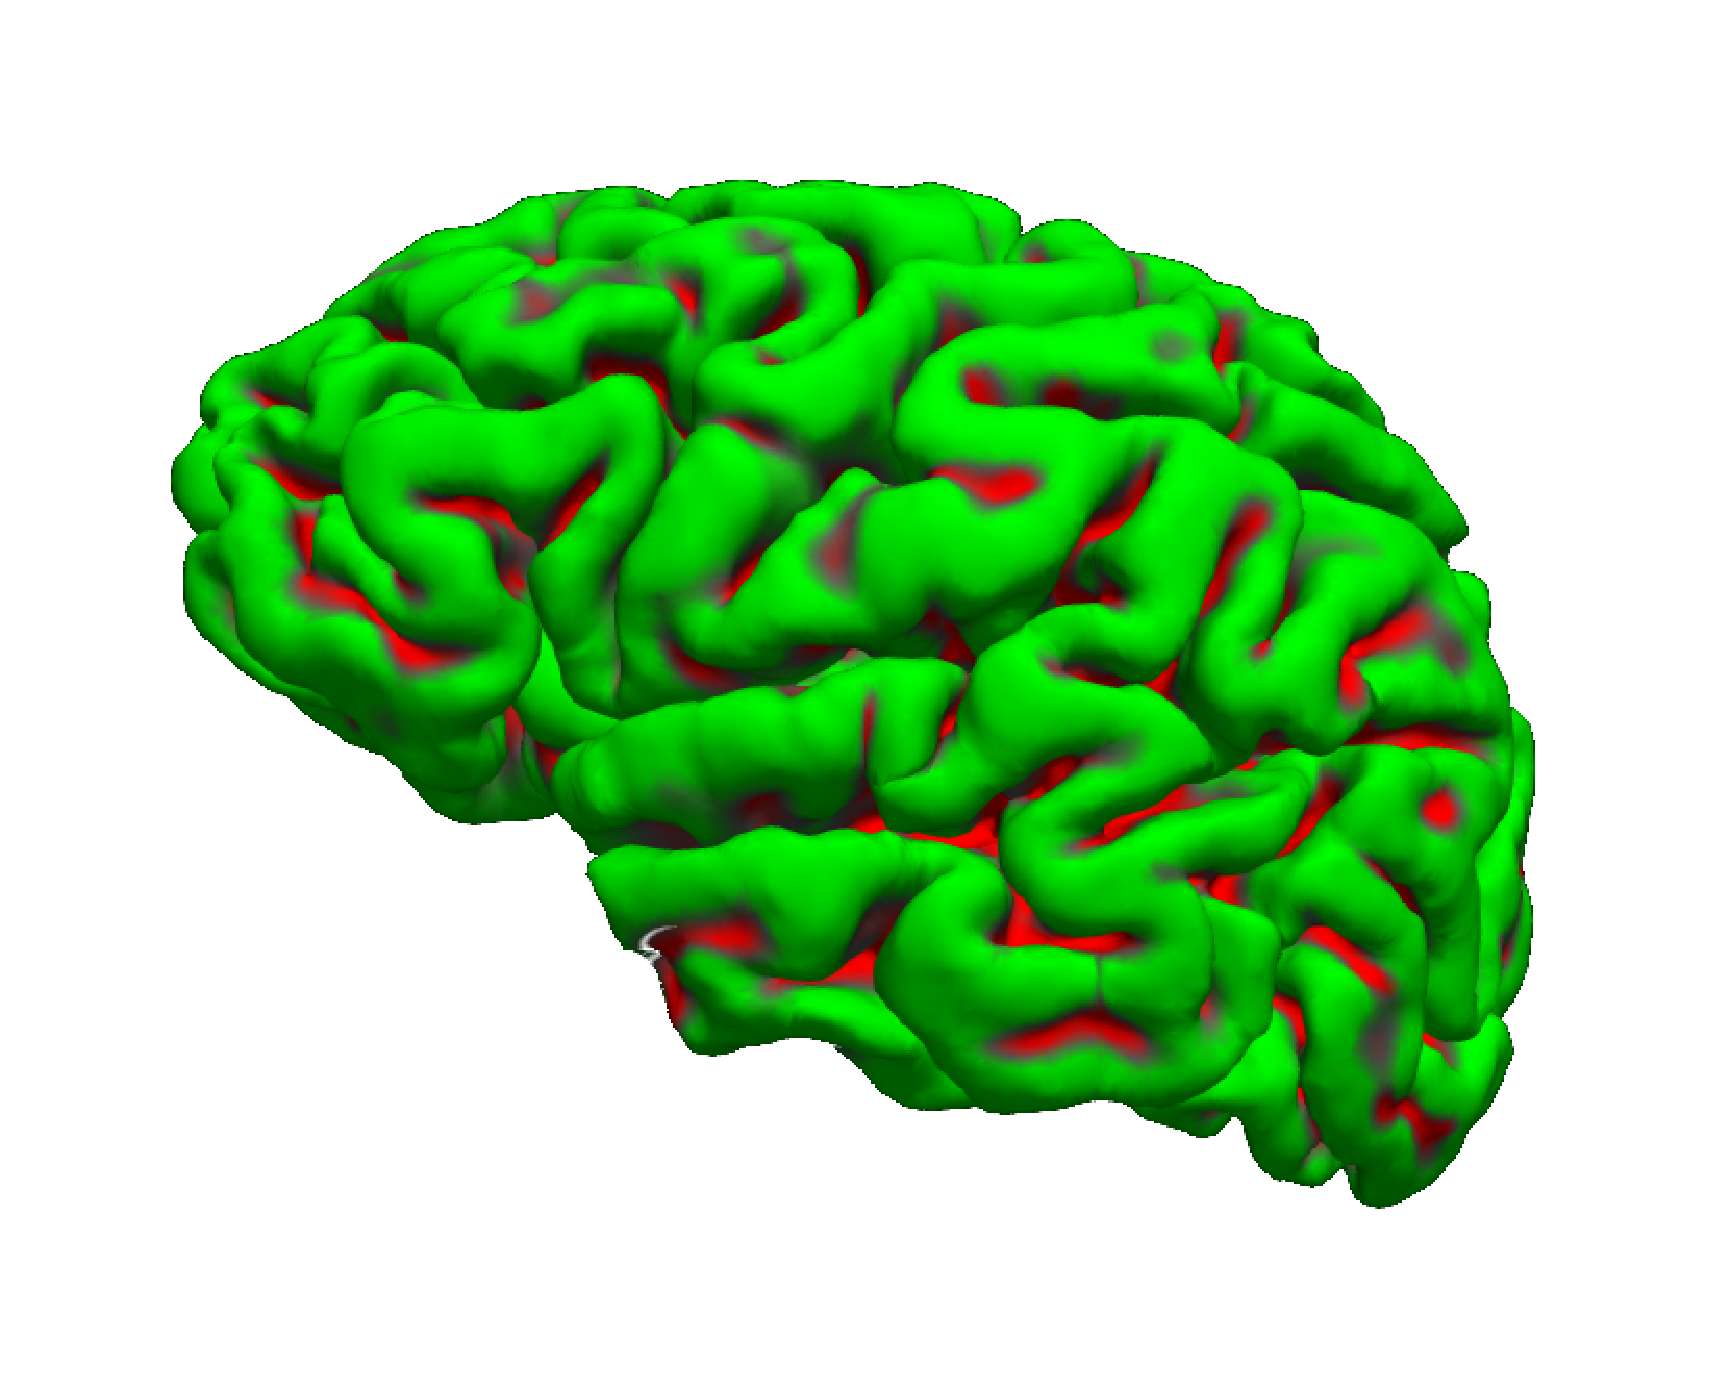
\epsfig{file = lh_S1_Simu_PialSurface.eps, width =5.5cm} 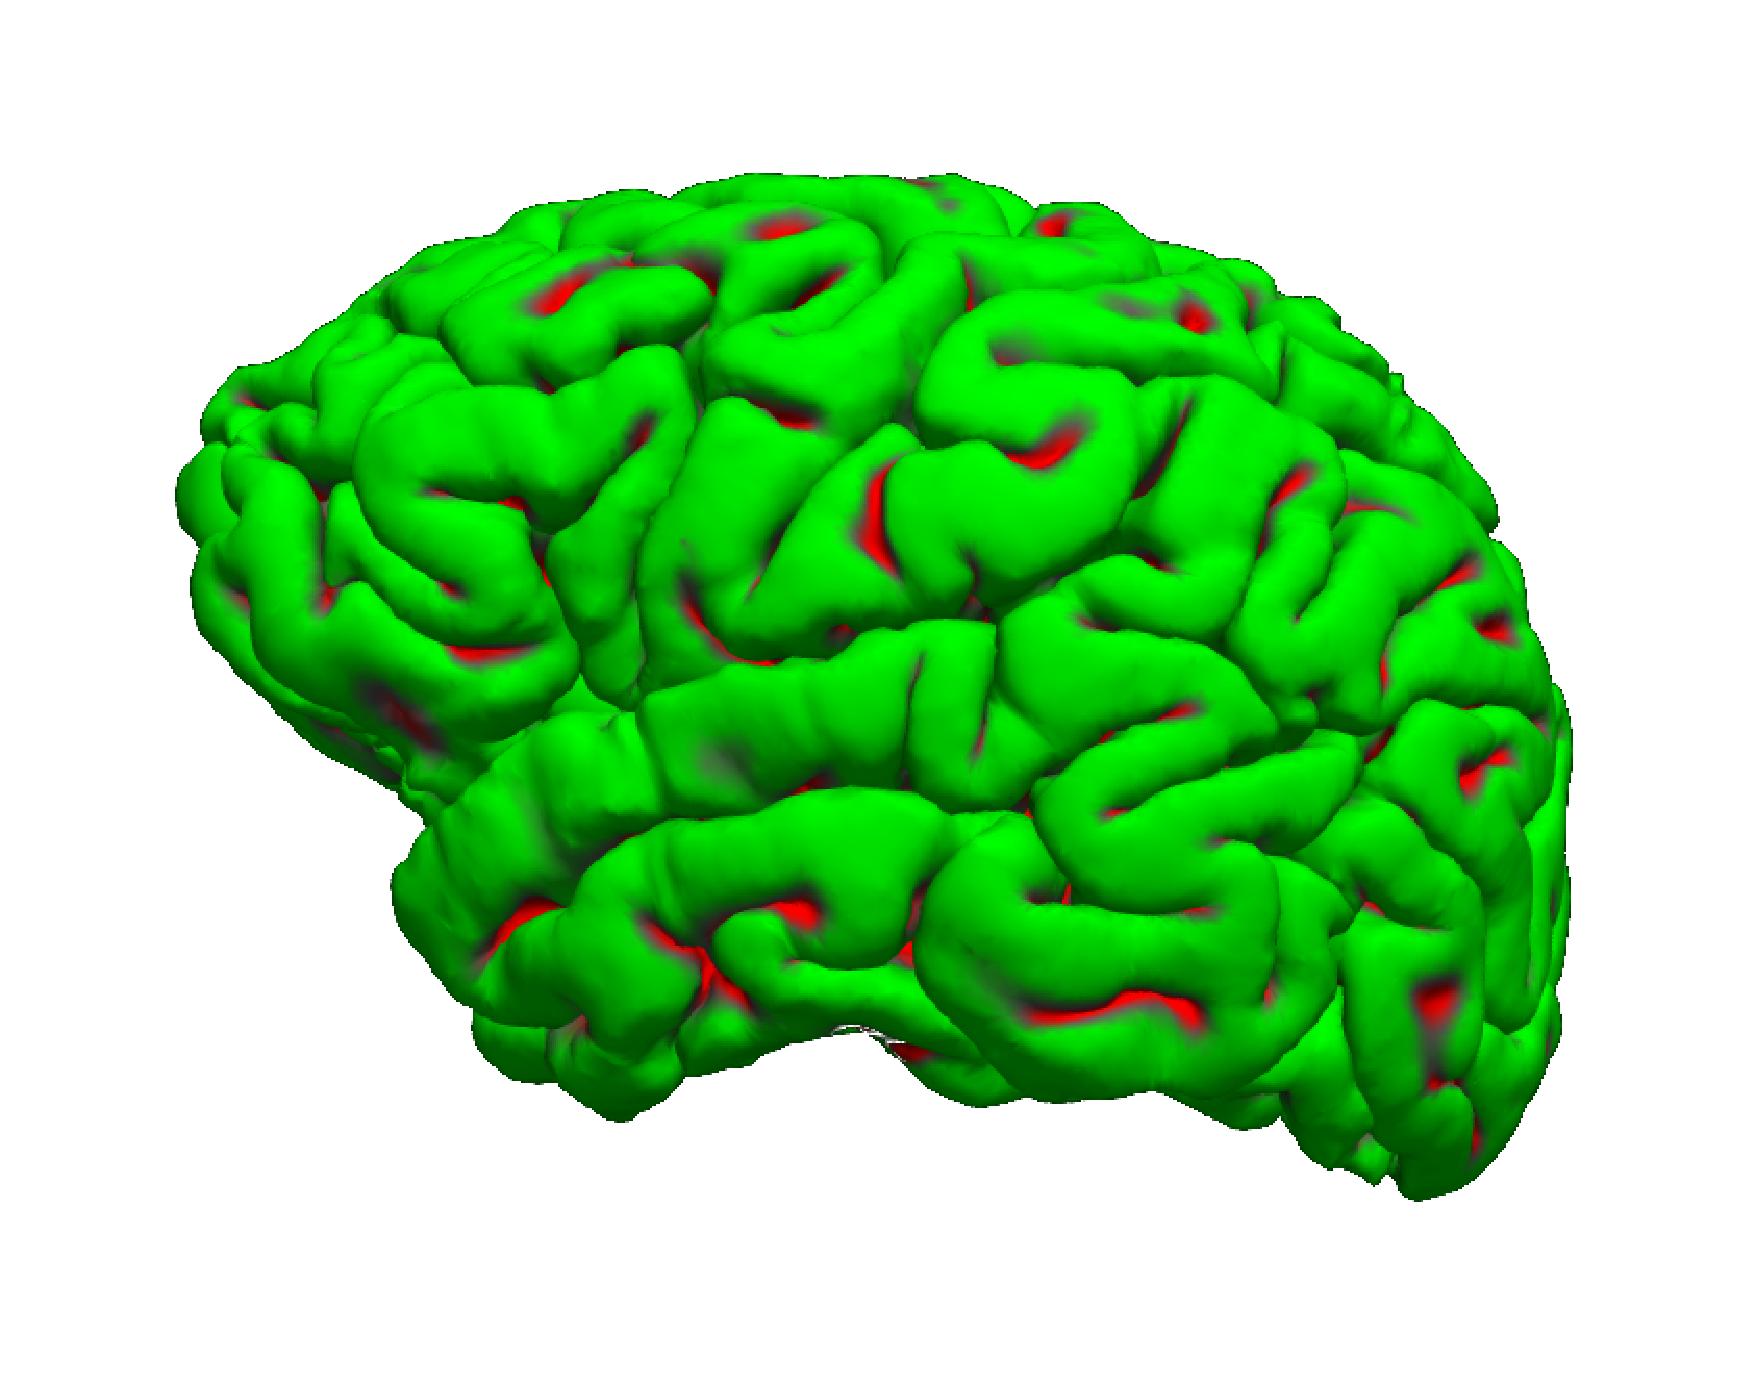
\epsfig{file = lh_S1_Orig_PialSurface.eps, width =5.5cm}}
 \subfigure[Right hemisphere WM surface.]{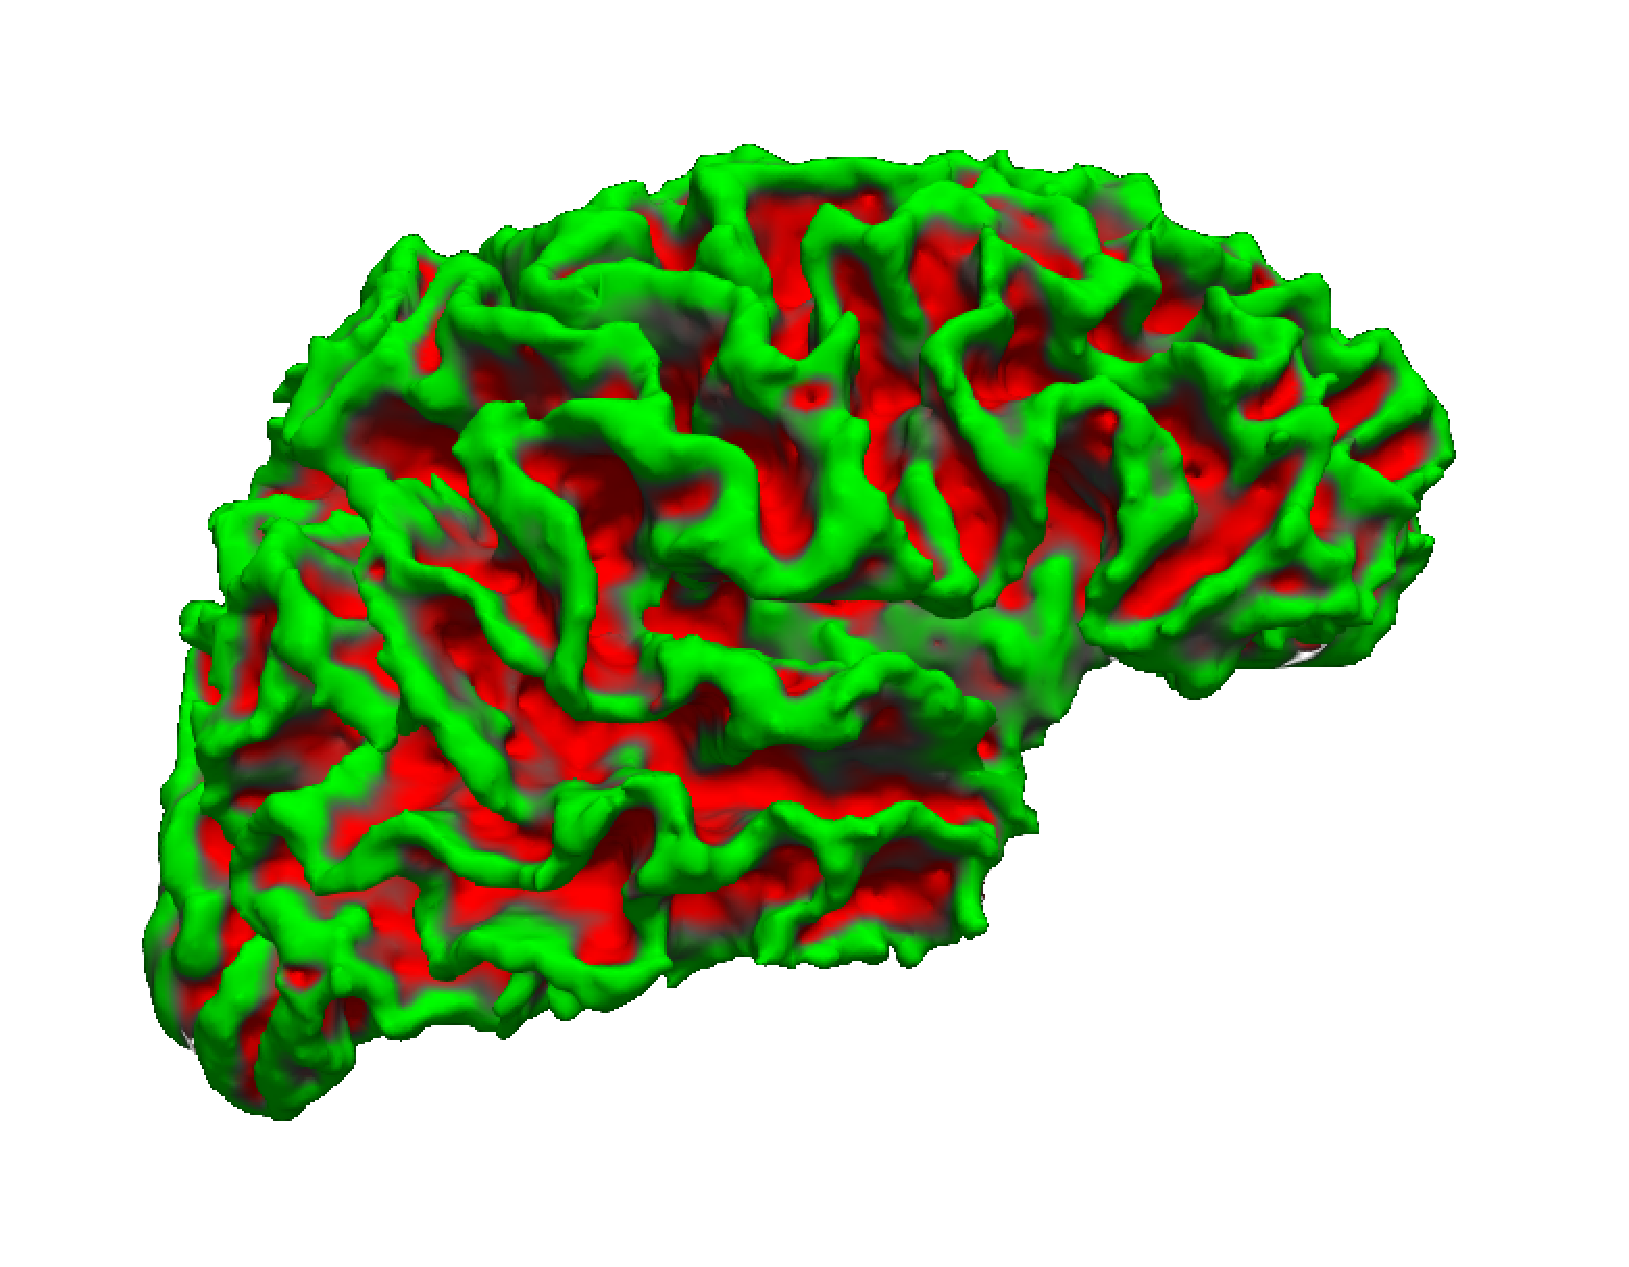
\epsfig{file = rh_S1_Simu_OrigSurface.eps, width =5.5cm} \epsfig{file = rh_S1_Orig_OrigSurface.eps, width =5.5cm}}
 \subfigure[Right hemisphere GM surface.]{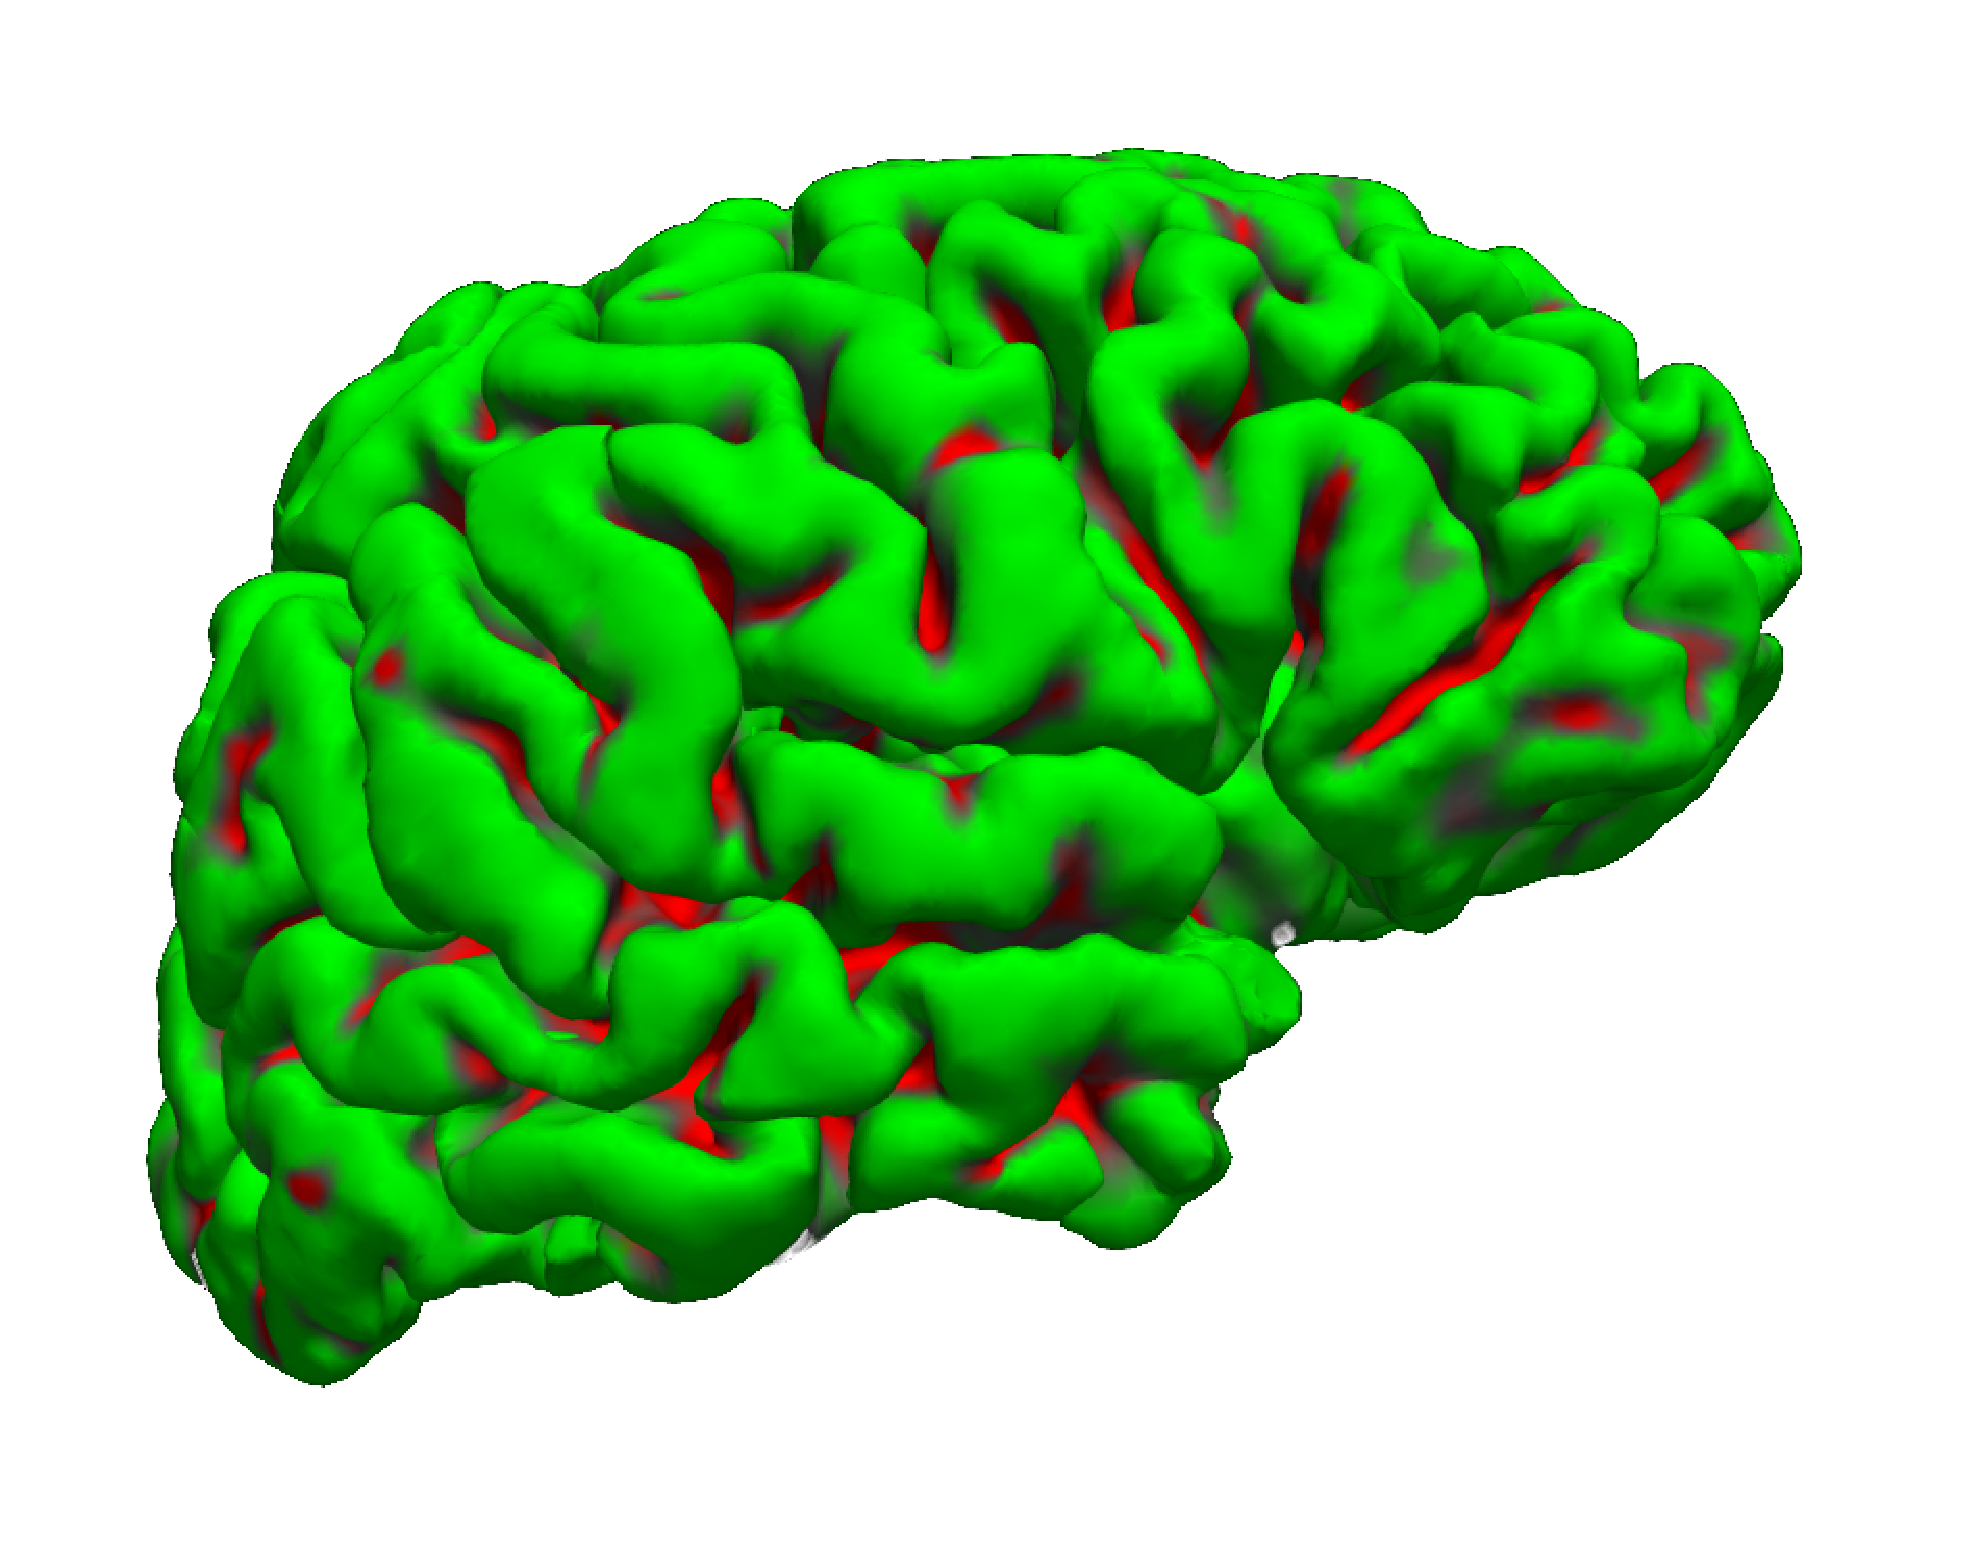
\epsfig{file = rh_S1_Simu_PialSurface.eps, width =5.5cm} \epsfig{file = rh_S1_Orig_PialSurface.eps, width =5.5cm}}
\caption[Visual comparison for cortical surface for Subject 1.]{Subject 1. Visualisation of curvature map for the WM surface and the GM surface in the left and right hemispheres of the cortex.
                                                   The images on the left column correspond to the simulated MRI segmented by \textit{Freesurfer}. 
                                                   The images on the right column correspond to the real MRI segmented by \textit{Freesurfer}. 
                                                   The global structure of the cortex is preserved. However, some differences can be seen as the segmentation of the simulated cortex
                                                   seems thinner. Also, the segmentation does not fully segment the superior temporal and middle temporal regions of the cortex.}
 \label{fig:physicalParamsObjectsSegmentedImageCortex1}  
\end{figure}


\begin{figure} 
 \centering   
 \subfigure[Left hemisphere WM surface.]{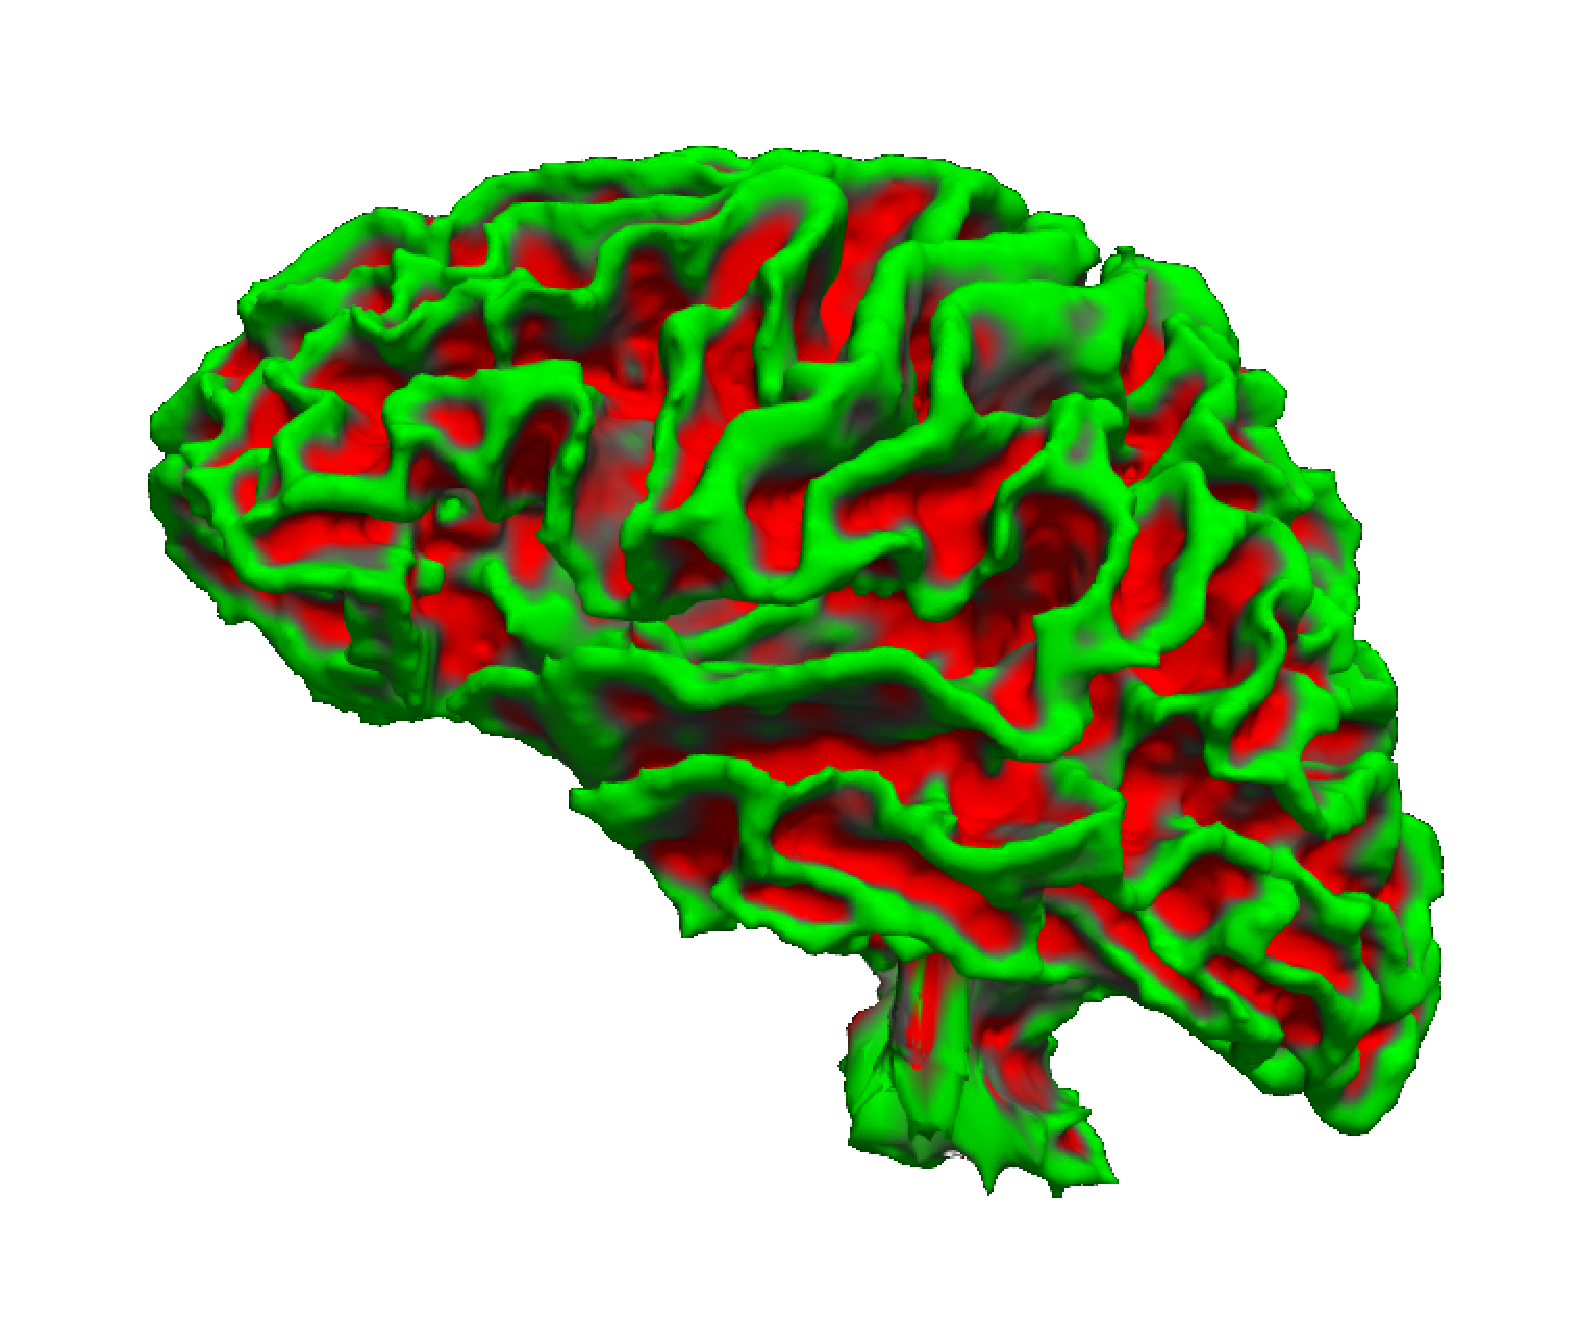
\epsfig{file = lh_S2_Simu_OrigSurface.eps, width =5.25cm} 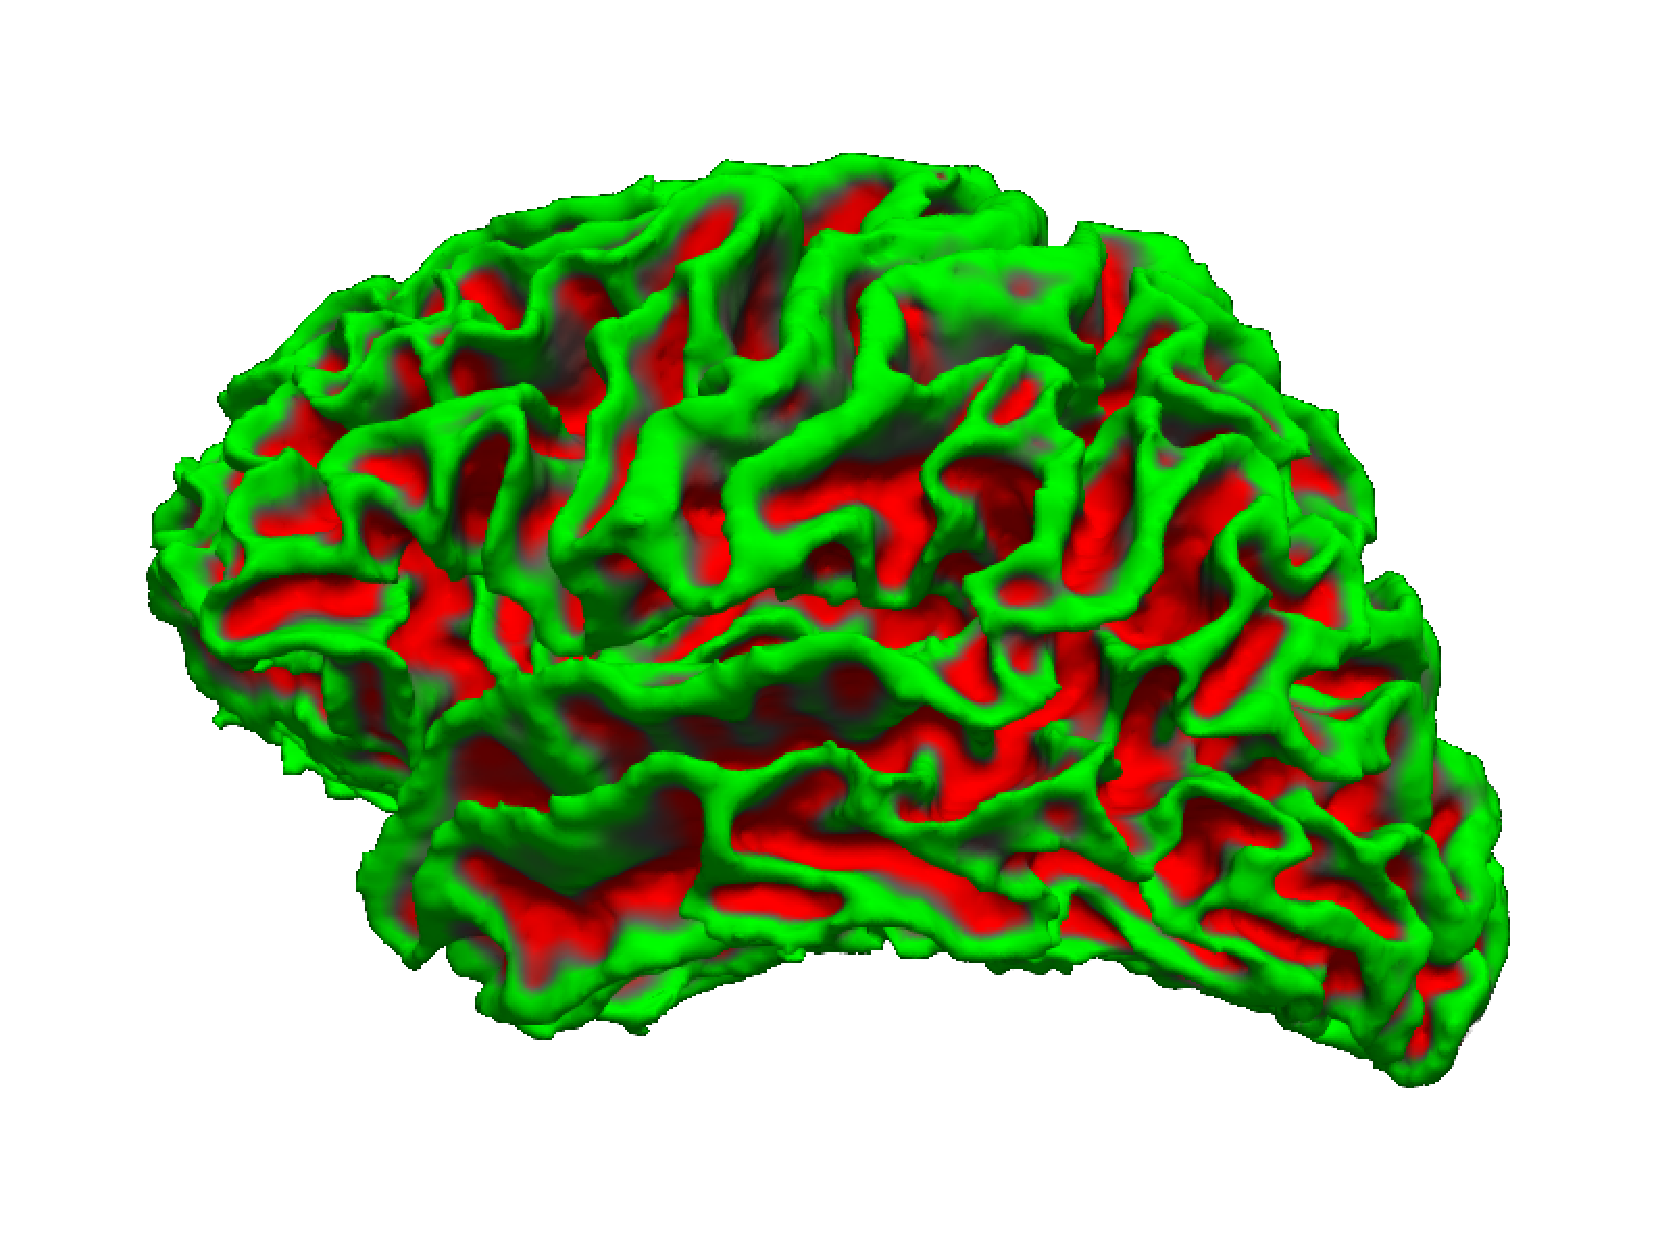
\epsfig{file = lh_S2_Orig_OrigSurface.eps, width =5.25cm}} 
 \subfigure[Left hemisphere GM surface.]{\epsfig{file = lh_S2_Simu_PialSurface.eps, width =5.25cm} \epsfig{file = lh_S2_Orig_PialSurface.eps, width =5.25cm}}
 \subfigure[Right hemisphere WM surface.]{\epsfig{file = rh_S2_Simu_OrigSurface.eps, width =5.25cm} \epsfig{file = rh_S2_Orig_OrigSurface.eps, width =5.25cm}}
 \subfigure[Right hemisphere GM surface.]{\epsfig{file = rh_S2_Simu_PialSurface.eps, width =5.25cm} \epsfig{file = rh_S2_Orig_PialSurface.eps, width =5.25cm}}
\caption[Visual comparison for cortical surface for Subject 2.]{Subject 2. Visualisation of curvature map for the WM surface and the GM surface in the left and right hemispheres of the cortex.
                                                   The images on the left column correspond to the simulated MRI segmented by \textit{Freesurfer}. 
                                                   The images on the right column correspond to the real MRI segmented by \textit{Freesurfer}. 
                                                   The global structure of the cortex is preserved. However, the segmentation produces an artifact at the base of 
                                                   the cortical surfaces.}
 \label{fig:physicalParamsObjectsSegmentedImageCortex2}  
\end{figure}


\begin{figure} 
 \centering   
 \subfigure[Left hemisphere WM surface.]{\epsfig{file = lh_S3_Simu_OrigSurface.eps, width =5.5cm} \epsfig{file = lh_S3_Orig_OrigSurface.eps, width =5.5cm}} 
 \subfigure[Left hemisphere GM surface.]{\epsfig{file = lh_S3_Simu_PialSurface.eps, width =5.5cm} \epsfig{file = lh_S3_Orig_PialSurface.eps, width =5.5cm}}
 \subfigure[Right hemisphere WM surface.]{\epsfig{file = rh_S3_Simu_OrigSurface.eps, width =5.5cm} \epsfig{file = rh_S3_Orig_OrigSurface.eps, width =5.5cm}}
 \subfigure[Right hemisphere GM surface.]{\epsfig{file = rh_S3_Simu_PialSurface.eps, width =5.5cm} \epsfig{file = rh_S3_Orig_PialSurface.eps, width =5.5cm}}
\caption[Visual comparison for cortical surface for Subject 3.]{Subject 3. Visualisation of curvature map for the WM surface and the GM surface in the left and right hemispheres of the cortex.
						     
                                                   The images on the left column correspond to the simulated MRI segmented by \textit{Freesurfer}. 
                                                   The images on the right column correspond to the real MRI segmented by \textit{Freesurfer}. 
                                                   Some local differences can be detected between the surfaces, but 
                                                   the overall structure of the cortex is preserved. }
 \label{fig:physicalParamsObjectsSegmentedImageCortex3}  
\end{figure}

A curvature map illustrates the degree of curviness in a surface.
In the case of the cortex, the map shows in green the areas of high convexity and in red the areas with high concavity. 
This corresponds to the gyri and sulci respectively.

Figures \ref{fig:physicalParamsObjectsSegmentedImageCortex1}, \ref{fig:physicalParamsObjectsSegmentedImageCortex2}, and \ref{fig:physicalParamsObjectsSegmentedImageCortex3} 
show the curvature map of the cortical surfaces for Subjects 1, 2 and 3 respectively.
The images on the left column correspond to the simulated data and the images on the right column correspond to the 
real data (the data used to fit the s-reps). 
The images are similar but not identical. 
In some cases, the cortex seems to be thinner or the regions in the cortex are under- or over-segmented 
by \textit{Freesurfer}. Nevertheless, these disagreements are quite small.

The following section gives a conclusion of the image simulation approach.
%Solid textures of physical parameters were created with the texture synthesis procedure.
%The solids are applied to different s-reps via the warping procedure explained in section \ref{sec:simulationExperimentRGB}.
%The following structures are fitted using s-reps:
%amygdala, caudate, hippocampus,  lateral ventricles, pallidum, putamen and the cortex.

\section{Conclusions}
\label{sec:ConclusionsSimu}

In conclusion, the approach is successful as
indicated by the fact that the images can be segmented by \textit{Freesurfer}. 
The cortical surfaces are reconstructed from the simulated data and globally, the cortical surfaces are similar to the real data
but local differences can be detected between the images.
Moreover, the simulated images are generated from
deformable models and textures lacking structural information. 
If the samples have structure, the texture synthesis algorithm 
can be used to its full potential and the results are likely to improve.

A single acquisition of physical parameters suffices to produce three new MRIs, but
extracting the textured samples was a difficult task due to low image resolution. 
\cite{CHAR-09} uses a label mask corresponding to the type of organ tissue, an average value and a standard deviation to 
generate the physical parameter distribution.
Following this logic, the image samples of physical parameters were 
created by sampling voxels inside the brain structures. Each sample is representative 
of each tissue.
As shown by the results, 
the simulated images with the physical parameters were able to 'trick' 
the segmentation pipeline of \textit{Freesurfer}. 

Future work aims to improve the image samples of physical parameters. This images 
should have the values of physical parameters and the appropriate texture distribution
according to each brain structure being modeled.
The $X2U$ map can also be used to texture the objects locally. 
Instead of having a single sample for a brain structure, 
different samples can be used to texture 
the regions in the brain structure accordingly. 

A second objective seeks to generate statistical descriptions of shape 
for the subcortical structures and the cortex using s-reps and CPNS.
The statistical descriptions will model healthy and pathological shape variations
for the subcortical structures and the cortex.
New brain structures can be generated from the statistics
allowing the combination of shapes from healthy and disease populations. 

The following chapter gives a global conclusion for this dissertation and proposes
future work according to the results found in these experiments.